\documentclass[12pt,letterpaper,oneside]{book}

% Packages
\usepackage[utf8]{inputenc}
\usepackage[T1]{fontenc}
\usepackage{newpxtext}
\usepackage{amsmath}
\usepackage{newpxmath}
\usepackage{geometry}
\usepackage{placeins}
\usepackage{graphicx}
\usepackage{chemfig}
\usepackage{csquotes}
\usepackage{microtype}
\usepackage[all]{nowidow}
\usepackage[colorlinks=true,linkcolor=blue,urlcolor=blue,citecolor=blue,anchorcolor=blue]{hyperref}
\usepackage[figure,table]{hypcap}
\usepackage[capitalise,noabbrev]{cleveref}

% Stuff for my glossary that I don't completely understand
\usepackage[nonumberlist]{glossaries}
\renewcommand*{\glspostdescription}{}
\makeglossaries
\newglossaryentry{schema}{
  name={Schema},
  description={A single learned prediction (also called priors or beliefs) in the brain's world model that is combined with an emotional reaction and possibly an episodic memory \cite{eckerUnlocking}. What are called low-level (physically lower in the brain) schemas perform a vast array of functions relating to the maintenance of basic bodily functions and sensory data processing \cite{clark2024experience}. Therapeutically relevant schemas are generally more abstract predictions about the self, relationships, or whether the world is generally safe/predictable or not.}
  %defined_in={What is Trauma and Why do its Effects Stick Around?},
  %stem={schema}
}

\newglossaryentry{reconsolidation-exhaustion}{
  name={Reconsolidation Exhaustion},
  description={Emotional exhaustion and lack of energy follow successful reconsolidation. It's usually called a therapy hangover. We think this is reliable enough to indicate that emotional exhaustion is a solid sign of therapeutic success. As far as we can tell, the phenomenon hasn't been formally studied. It seems to dissipate within a few hours, though exceptionally high levels of reconsolidation, like during MDMA therapy, could conceivably generate longer-lasting exhaustion. People seem to be capable of 1-2 hours of reconsolidation a day before exhaustion becomes so intense that the process is no longer possible.}
  %defined_in={The MDMA Therapy Session},
  %stem={emotionally exhausted, reconsolidation exhaustion, therapy hangover, emotional exhaustion}
}

\newglossaryentry{reconsolidation}{
  name={Reconsolidation},
  description={When a schema/memory first forms, it is \enquote{consolidated} \cite{eckerUnlocking}. When prediction error on that schema becomes large enough, the schema enters a mode where it is changeable. Maintaining that prediction error then updates the schema to reflect the new information. At the end of this process the schema \enquote{re-consolidates,} and becomes unchangeable again. We use \enquote{reconsolidate} to denote this whole process of activation, updating, and reconsolidation.}
  %defined_in={Mechanism of Healing},
  %stem={reconsolidat}
}

\newglossaryentry{defense-cascade}{
  name={Defense Cascade},
  description={A series of physiological changes in the sympathetic and parasympathetic nervous systems that prepares the body to respond to imminent threats \cite{kozlowskaDefenseCascade}. Includes arousal, fight or flight, freezing, and tonic/collapsed immobility. Different situations and experiences activate different responses.}
  %defined_in={The Defense Cascade},
  %stem={defense cascade}
}

\newglossaryentry{arousal}{
  name={Arousal},
  description={The first step when a potential threat is noticed and assists in further assessing that threat \cite{kozlowskaDefenseCascade}. It is also preparation for more intense defense responses like fight or flight, freeze, or immobility. Heart rate, breathing, and muscle tone increase, saliva is no longer produced, and core muscles tighten to stabilize posture.}
  %defined_in={The Defense Cascade},
  %stem={arous}
}

\newglossaryentry{fight-or-flight}{
  name={Fight or Flight},
  description={Active defense response characterized by high levels of adrenaline and muscle activation, increased heart rate, and decreased pain sensitivity \cite{kozlowskaDefenseCascade}.}
  %defined_in={The Defense Cascade},
  %stem={fight-or-flight}
}

\newglossaryentry{freeze}{
  name={Freeze},
  description={A fight or flight response temporarily put on hold \cite{kozlowskaDefenseCascade}. One remains highly attentive but frozen to avoid the notice of predators who are more likely to notice moving objects.}
  %defined_in={The Defense Cascade},
  %stem={freez}
}

\newglossaryentry{immobility}{
  name={Tonic/Collapsed Immobility},
  description={Inactive defense responses characterized by detachment, emotional and physical numbing, and immobility \cite{kozlowskaDefenseCascade}. Predators are more attracted to moving prey and may lose interest in seemingly dead bodies. May escalate to unconsciousness.}
  %defined_in={The Defense Cascade},
  %stem={immobil}
}

\newglossaryentry{dissociation}{
  name={Dissociation},
  % description={Emotional numbing caused by brain-produced opioids in situations of perceived threat and powerlessness, which is usually a maladaptive schema when you're not in an acutely dangerous situation \cite{lanius2018review,kozlowskaDefenseCascade}. This can escalate to immobility and greater degrees of detachment from one's self and external reality.}
  description={An umbrella term encompassing both deep avoidance and tonic/collapsed immobility \cite{kozlowskaDefenseCascade}.}
  %defined_in={The Defense Cascade},
  %stem={dissociat}
}

\newglossaryentry{trauma}{
  name={Trauma},
  description={We use two closely related definitions: First, events that lead to over-generalized schemas that impair functioning or emotional health. Second, distressing events or chronic conditions that overwhelm our ability to cope, where our ability to cope depends on our capabilities and resources \cite{laneReconsolidation}.}
  %defined_in={What is Trauma and Why do its Effects Stick Around?},
  %stem={trauma}
}

\newglossaryentry{connectogen}{
  name={Connectogen},
  description={A term for MDMA's class of drugs, designed to unify the competing terms \textit{entactogen} and \textit{empathogen} \cite{stockerConnectogen}. MDMA facilitates profound connection to self, body, senses, and others. The ego and sense of self are maintained and hallucinations are minimal, unlike with the classic psychedelics or hallucinogens.}
  %defined_in={Introduction},
  %stem={Connectogen}
}

\newglossaryentry{psychedelic}{
  name={Psychedelic},
  description={\enquote{Showing the Mind/Soul,} from the Greek \enquote{psyche} and \enquote{deloun} \cite{osmondObit}. Most are tryptamines, phenethylamines, and ergamides \cite{gumpper2024chemistry}. Each compound has different effects, but they generally relax abstract predictions \cite{carhart2019rebus}. We specifically do not categorize MDMA as a psychedelic, but rather a connectogen \cite{stockerConnectogen}}
  %defined_in={na},
  %stem={psychedelic}
}

\newglossaryentry{attachment-theory}{
  name={Attachment Theory/Styles},
  description={Attachment theory posits that emotionally secure attachments formed in the first 18 months of life serve as the foundation for emotional and psychological development throughout one's life \cite{brownAttachmentDisturbances}. Assess using \textcite{attachmentProject}.}
  %defined_in={Attachment Theory},
  %stem={secure attachment, attachment theory, attachment disorder, disordered attachment}
}

\newglossaryentry{predictive-processing}{
  name={Predictive Processing},
  description={The prevailing model of brain function \cite{clark2015surfing}. The brain internally models the world (via complex layers of learned predictions) to better plan for the fulfillment of basic needs such as bodily integrity, reproduction, community, etc. Prediction error is a discrepancy between the brain's model of the world and incoming sensory data or between two contradictory model predictions. Minimization of prediction error is the brain's core optimization function, achieved through the construction of more complex and accurate world models.}
  %defined_in={What is Trauma and Why do its Effects Stick Around?},
  %stem={predicti}
}

\newglossaryentry{mismatch}{
  name={Mismatch},
  description={The conscious contradiction of an active schema via either sensory input or another schema \cite{eckerUnlocking}.}
  %defined_in={Mechanism of Healing},
  %stem={mismatch}
}

\newglossaryentry{resistance}{
  name={Resistance},
  description={Opposition to reconsolidation or a broader therapeutic process that would actually be healthy for the individual. This is difficult to ascertain, as many therapeutic processes are not actually a good match for many people.}
  %defined_in={na},
  %stem={resistance}
}

\newglossaryentry{avoidance}{
  name={Avoidance},
  description={Physical or mental (often unconscious) actions that direct attention away from contradictory information or distressing thoughts and inhibit reconsolidation \cite{clark2015surfing}. Short-term avoidance can be healthy if used to temporarily postpone dealing with a problem until you have more capacity.}
  %defined_in={What is Trauma and Why do its Effects Stick Around?},
  %stem={avoida}
}

\newglossaryentry{biopsychosocial-model}{
  name={Biopsychosocial Model},
  description={Prevailing model of mental illness as a complex interaction of biology (genes and medical history), psychology (schemas, in our view), and society (one's support system and social models of how to respond to adversity) \cite{engel1977need}.}
  %defined_in={What is Trauma and Why do its Effects Stick Around?},
  %stem={biopsychosocial}
}

\newglossaryentry{complex-system}{
  name={Complex System},
  description={Systems with many interacting parts that are difficult to model and understand \cite{hayes2020complex}. The overall behavior of the system can't be easily predicted by looking at the individual components.}
  %defined_in={Complex Systems, Worsening Symptoms, and Destabilization},
  %stem={complex system}
}

\newglossaryentry{attractor-state}{
  name={Attractor},
  description={A state in a complex system that the system is drawn to and which it is difficult to get out of \cite{hayes2020complex}. Addiction is a good example. Maladaptive schemas seem to stick around because they combine with some process inhibiting reconsolidation, which together form an attractor state \cite{hayes2020complex,berghSelfEvidencing}. The durability of the state requires both elements; removing either element destabilizes it.}
  %defined_in={Complex Systems, Worsening Symptoms, and Destabilization},
  %stem={attractor}
}

\newglossaryentry{destabilization}{
  name={Destabilization},
  description={Throughout the book we use the term destabilization as a catchall for two phenomena we describe in \ref{sec:complex}. The first is increased fluctuation between states of good and bad mental health that often precedes a stabilizing transition to the good state. The second is a transition to a stable and even worse state of mental health, possibly precipitated by confronting disturbing memories that were previously avoided. Both phenomena are part of the healthy process of therapy when managed well and entered into at an appropriate time in your life.}
  %defined_in={Mechanism of Healing},
  %stem={destabiliz}
}

\newglossaryentry{afterglow}{
  name={Afterglow},
  description={A days-weeks long period after a session involving well-being, positive mood, mindfulness, positive behaviors, and less mental illness \cite{evansAfterglow}. Regular therapy might be more effective in this period. Common knowledge is that afterglow is unreliable. It can also occasionally be strong enough that people feel like they're on a low dose of MDMA.}
  %defined_in={Afterglow},
  %stem={afterglow}
}

% Stuff for the fancy table in Defense Cascade
\usepackage{longtable}
\usepackage{array}
\usepackage{booktabs}
\usepackage{enumitem}
% Define a compact itemize environment for tables
\newenvironment{compactitemize}
{\begin{itemize}[nosep, leftmargin=1em, itemsep=0pt, topsep=0pt]}
{\end{itemize}}

\usepackage[backend=biber, style=apa, citestyle=numeric]{biblatex}

% Redefine bibliography to include numbers like numeric style does
\DeclareFieldFormat{labelnumberwidth}{\mkbibbrackets{#1}}
\setlength{\biblabelsep}{1em}
\defbibenvironment{bibliography}
  {\list
     {\printtext[labelnumberwidth]{%
        \printfield{labelprefix}%
        \printfield{labelnumber}}}
     {\setlength{\labelwidth}{\labelnumberwidth}%
      \setlength{\leftmargin}{\labelwidth}%
      \setlength{\labelsep}{\biblabelsep}%
      \addtolength{\leftmargin}{\labelsep}%
      \setlength{\itemsep}{\bibitemsep}%
      \setlength{\parsep}{\bibparsep}}%
   \renewcommand*{\makelabel}[1]{\hss##1}}
  {\endlist}
  {\item}

% Standard bibliography stuff, though I don't like having to set penalties
\DeclareLanguageMapping{english}{english-apa}
\addbibresource{references.bib}
\setcounter{biburlnumpenalty}{9000}
\setcounter{biburlucpenalty}{9000}
\setcounter{biburllcpenalty}{9000}

% Hide https://, http://, https://doi.org/, www. in bibliography links to reduce clutter
\DeclareSourcemap{
\maps[datatype=bibtex]{
\map{
\step[fieldsource=url, final=true]
\step[fieldset=verba, origfieldval, final=true]
\step[fieldsource=verba, match=\regexp{\A(ht|f)tp(s)?:\/\/}, replace={}]
\step[fieldsource=verba, match=\regexp{\Awww\.}, replace={}]
\step[fieldsource=verba, match=\regexp{\Adoi\.org\/}, replace={}]
 }
 }
}
\DeclareFieldFormat{url}{%
\ifentrytype{book}
 {}
 {\mkbibacro{URL}\addcolon\space\href{#1}{\nolinkurl{\thefield{verba}}}}%
 }
\DeclareFieldFormat{doi}{%
\mkbibacro{DOI}\addcolon\space
\ifhyperref
 {\href{https://doi.org/#1}{\nolinkurl{#1}}}
 {\nolinkurl{#1}}}

\interfootnotelinepenalty=10000

% Make citations and text that only appear in markdown for reddit
\newcommand{\mdcite}[1]{}
\newcommand{\mdonly}[1]{}

% Make \citetitle do capitalization right
% \usepackage{titlecaps}
% \Addlcwords{a an the and but or nor for so yet to of in on at by with from as into onto upon}
% \DeclareFieldFormat[article,inbook,suppbook,incollection,suppcollection,inproceedings,inreference,suppperiodical,online,misc,patent,unpublished]{citetitle}{\MakeSentenceCase*{#1}}
% \DeclareFieldFormat[book,mvbook,bookinbook,booklet,collection,mvcollection,proceedings,mvproceedings,manual,reference,mvreference,report,thesis,periodical,dataset,software]{citetitle}{\mkbibemph{\titlecap{#1}}}

% Just function-less tracking of who wrote what
\newcommand{\writtenByDay}[1]{#1}

% A helper command to simplify the How to Read This Book section
\newcommand{\combinedref}[1]{\ref{#1} (\nameref*{#1})}

% Not sure what this is for
\newcommand{\combinedcref}[1]{\cref{#1} (\nameref*{#1})} % Use for subsection* where the reference points to the next higher up structure. It will show the subsection* name in ().

% Commands to make prosecite
\DeclareCiteCommand{\citefullauthor}
  {\boolfalse{citetracker}%
   \boolfalse{pagetracker}}
  {\printnames[given-family]{labelname}}
  {\multicitedelim}
  {}
\newcommand{\prosecite}[1]{\citetitle{#1} by \citefullauthor{#1}~\cite{#1}}

\geometry{top=1in, bottom=1in, left=1in, right=1in}

% Some stuff that makes todo notes work for some reason
\setlength{\marginparwidth}{2cm}
\setlength{\marginparsep}{0.3cm}
\usepackage[textsize=tiny,textwidth=2cm]{todonotes}

\setcounter{tocdepth}{2}

\begin{document}

% \pagenumbering{gobble}
% \newgeometry{margin=0pt}
% \thispagestyle{empty}
% \noindent \includegraphics[width=\paperwidth,height=\paperheight]{cover.pdf}
% \restoregeometry

\frontmatter

\title{Open MDMA: An Evidence-Based Synthesis, Theory, and Manual for MDMA Therapy Based on Predictive Processing, Complex Systems, and the Defense Cascade}
\author{
    Mark Groeneveld\thanks{Corresponding author; Email: \href{mailto:mgroeneveld@protonmail.ch}{mgroeneveld@protonmail.ch}} \and
    Thomas Harper, M.S.W.\thanks{Master of Social Work; Has not reviewed this version of the preprint}
}
\date{Preprint Draft Version 5.1 \today. This is a complete-ish first draft that's in decent shape aside from a lack of editing, lack of review, and a list of minor to-do's. SAFETY RECOMMENDATIONS ARE UNDERGOING MAJOR REVISIONS.}

\maketitle{
    \begin{center}
        This work is licensed under \href{https://creativecommons.org/licenses/by/4.0/}{CC BY 4.0}.

        \vspace{\baselineskip}

        If you share this document, please use this link to ensure people have the latest version: \href{https://doi.org/10.31234/osf.io/aps5g}{doi.org/10.31234/osf.io/aps5g}. This site also tallies downloads, informing us how many people are using the manual and how worthwhile it is to update it with new research.

        \vspace{\baselineskip}

        We'd love to hear your thoughts at \href{mailto:mgroeneveld@protonmail.ch}{mgroeneveld@protonmail.ch}. We're curious about how you're using the manual, what you like, what you don't, any errors you spot, etc.

        \vspace{\baselineskip}

        You can submit anonymous feedback \href{https://docs.google.com/forms/d/e/1FAIpQLScZe2h4L9PcLQGGpuerk44FXiWThRC2w6YNwSm67OXIJun-rA/viewform?usp=dialog}{here}.
    \end{center}
}

\newpage
\begin{center}
    \textbf{Abstract}
\end{center}
\vspace{\baselineskip}

This comprehensive open-science manual provides evidence-informed guidance for MDMA-assisted psychotherapy, addressing the critical gap between growing interest in  MDMA therapy and accessible, scientifically grounded information. Drawing on memory reconsolidation/predictive processing, complex systems dynamics, and the defense cascade model of autonomic threat responses, the authors explain how MDMA facilitates the unlearning of the maladaptive schemas/predictions underlying many mental illnesses. The book synthesizes current research with clinical and lived experience to offer practical protocols for MDMA therapy. The manual covers essential topics including the neuroscience of trauma and healing, comprehensive safety considerations and contraindications, detailed session preparation and navigation techniques, managing therapeutic destabilization and adverse effects, and strategies for continued reconsolidation between sessions. Special attention is given to the challenges of accessing ethical, skilled professional support and the complex risk-benefit considerations of solo therapy. Written for mental health professionals, their clients, and individuals pursuing healing outside traditional frameworks, this guide emphasizes practices to improve efficacy and reduce risk. The authors acknowledge MDMA therapy's potential for rapid, profound healing while providing a thorough discussion of risks, including dangerous drug interactions, psychological destabilization, and the importance of proper support structures. This manual aims to improve the safety and effectiveness of MDMA therapy as practiced in various contexts, while advocating for approaches grounded in compassion, scientific rigor, and respect for individual autonomy.\footnote{We used Claude Opus 4 to draft this abstract because the need for a preliminary abstract exceeded our patience to write one but have edited it ourself. The book itself is 100\% human-written.}
\clearpage

\newpage
\begin{center}
    \textbf{Disclaimer}
\end{center}
\vspace{\baselineskip}

This guide doesn't offer personalized medical/therapeutic advice, guarantee healing, assure the prevention of negative (possibly severe) outcomes, or prevent legal problems if used in a place where MDMA is illegal. Instead, this guide is our framework for increasing the efficacy and safety of MDMA therapy, grounded in research, community insights, and author experiences. We have spent considerable effort trying to make the best guide we can, but we could be wrong about some important things. Please cross-check our references with other high-quality sources of information if you question something we say or are considering doing something potentially risky. Possessing MDMA is a felony in many jurisdictions. Licensed mental health professionals theoretically risk their licenses by offering MDMA therapy in contexts where it isn't legal.

\vspace{\baselineskip}

While this guide has universal aspects, it doesn't cover all frameworks for doing MDMA therapy. Although MDMA therapy has been practiced by underground therapists for 50 years, comprehensive scientific study is relatively recent, leaving many aspects unexplored. Our theoretical integration of MDMA therapy, complex systems dynamics, memory reconsolidation, prediction error, attention, and the defense cascade appears novel despite each piece, and some combinations of the pieces, being fairly well-established. The application of that integrated framework to a practical guide and MDMA therapy is also largely novel. Novel frameworks are usually incorrect to some degree even when their authors find them convincing. Additionally, as an interdisciplinary work, we are surely getting some details of the individual frameworks we draw from wrong.
\clearpage

\newpage
\begin{center}
    \textbf{Changes from Version 5 to 6}
\end{center}
\vspace{\baselineskip}

Reworked and polished \nameref{sec:safety}, \nameref{frequency}, \nameref{ppHypotheses}, Efficacy, \nameref{internalizedReports}, Preface, Plain Language Summary. Edited everything for grammar and spelling. Removed Our Pitch because it didn't fit in well and was redundant. Shuffled a couple sections around. Also made a lot of little changes here and there.

\begin{center}
    \textbf{Changes from Version 4 to 5}
\end{center}
\vspace{\baselineskip}

Removed the two Beyond Therapy sections and Organizing Community Care because they were overly influenced by our own maladaptive schemas. Added \nameref{ppHypotheses}, \nameref{bigPicture}, \nameref{attention}, the Sessions Become Less Effective Over Time troubleshooting subsection, Plain Language Summary, the Psychosis troubleshooting subsection, and the subsection Reasons to be Skeptical to \nameref{sec:assumptions}. Rewrote \nameref{psychogenic}, \nameref{frequency}, and the Safety section bullet point on psychosis. Split Epistemic Status into \nameref{sec:assumptions} and \nameref{howtoevaluate}. Shuffled around various sections into different chapters or renamed them. Bumped up the risk assessment of frequent higher-dose sessions due to \textcite{corayMemory}. Also made a lot of little changes here and there.

\vspace{\baselineskip}
\begin{center}
    \textbf{Changes from Version 3 to 4}
\end{center}
\vspace{\baselineskip}

Added Preface, \nameref{sec:complex}, subsections Major Unresolved Issues and Reference Quality in \nameref{sec:assumptions}, subsection Acute Effects in \nameref{sec:safety}, self-reports of internalized MDMA therapy, paragraph on involuntary hospitalization, and Cognitive Flexibility and Truth Seeking. Rewrote \nameref{sec:moreReconsolidation} and \nameref{sectionManagement}. Also made a lot of little changes here and there.

\clearpage

\tableofcontents

\chapter{Collected Paragraphs}
Please edit the following paragraphs collected here from various parts of the book:
\begin{itemize}
    \item (If you think this is a bad idea don't bother with editing. This is speculation outside my area of knowledge; it may be completely unadvisable for reasons I don't understand. Tonic/collapsed immobility is a barrier to therapeutic progress in MDMA therapy, and I thought these drugs might help.) There is low-quality evidence that 50--250\,mg of the opioid antagonist naltrexone deactivates opioid-mediated states (like immobility and freezing)~\cite{escamilla2023treatment}. Naloxone and nalmefene have similar mechanisms of action and could conceivably also work, though this hasn't been demonstrated. Naloxone's half-life seems more appropriate to MDMA therapy than naltrexone's. Some of these drugs require prescriptions in certain jurisdictions, and collaboration with a prescribing medical professional may be necessary. We are not aware of any attempts at combining opioid antagonists with MDMA. If you try this novel combination, we suggest using lower doses, as all drugs have side effects, ranges of safe dosing, and interactions with other drugs, including potentially MDMA. \textcite{naltrexoneInfo} provides thorough information about naltrexone. We are unable to provide instructions on safe and effective use here. Reducing immobility may make reconsolidating the schemas triggering it easier.
    \item \textbf{Troubleshooting: Still High More than 24\,Hours Later} This could be afterglow (see \cref{afterglow}). The MDMA might also be metabolizing slowly. Some metabolize MDMA much slower than average~\cite{straumann2024racemic}. Some drugs or pre-existing liver issues also inhibit metabolism, like ritonavir and cobicistat~\cite{sarparastDrugInteractions,bracchi2015antiretrovirals}. Tonic immobility, possibly triggered by exposing vulnerabilities during the session, also involves an altered state of consciousness (see \cref{sec:defensecascade,sectionManagement}). In rare circumstances MDMA might also facilitate processes that lead to persisting perception of non-duality (see \cref{selfinsight}).
    \item \textbf{Troubleshooting: Not Feeling Anything or Feeling \enquote{Meh}}
    \begin{itemize}
        \item Your expectation for the session may not match up with the maladaptive schemas actually present. This can present as disappointment or anxiety about the trip itself. Lean into and focus on that disappointment or anxiety to reconsolidate it.
        \item You may be inadvertently avoiding an unnoticed feeling. We suspect practicing different types of meditation for 30\,minutes might help you notice and engage with subtle feelings. See \prosecite{rain} and \prosecite{bodyscan}.
        \item Long-term use of SSRIs and SNRIs blunts the effects of MDMA~\cite{feducciaSSRIDiscontinuation}. This effect may persist for multiple months after discontinuing these medicines.
        \item Other drugs can blunt the effects of MDMA.
        \item The dose may have been too low. See \cref{sec:dosing}.
        \item The substance might be adulterated or cut with fillers. See \cref{testing}.
        \item MDMA conceivably may not work for some people for unknown reasons. We strongly suspect that some people who think that MDMA might not work with their brain were actually experiencing immobility or avoiding an anxiety they didn't identify as a reconsolidation target. Try working through \cref{sec:sessionbarriers} before concluding that MDMA doesn't work with your brain.
    \end{itemize}
    \item \textbf{Troubleshooting: Sleepiness, Disconnection, or Heaviness} MDMA is a strong stimulant that generally increases feelings of energy~\cite{vizeliActuteEffects}. Activating schemas (one you are perhaps not aware of) of powerlessness and threat during therapy commonly activates collapsed immobility, which can include sleepiness~\cite{kozlowskaDefenseCascade}. We suggest immobility is the most likely cause for sleepiness during a session, though atypical responses to the drug or other medical conditions could conceivably play a role. See \cref{sec:sessionbarriers} for suggestions on working with immobility. We recommend following the immobility guidelines first even if you suspect an atypical stimulant/neurotransmitter response because these conditions may be difficult to distinguish, especially in multiple altered states of consciousness (both MDMA and immobility). \cref{sec:signsofdc} is a list of immobility symptoms that may prove helpful in differentiating immobility from another response.
    \item MDMA can cause jaw clenching and headaches~\cite{mitchellMDMAClinicalTrial2,liechtiGender}. Some people use mouth guards or pacifiers to reduce this effect or protect their teeth~\cite{emdeEmergency}. \textcite{liechtiInteractions} says acetaminophen and NSAIDs are compatible with MDMA. However, NSAIDs irritate empty stomachs, and people often do not eat before and during MDMA therapy.
    \item \textcite{liechtiInteractions} recommends domperidone for nausea (10\,mg max at a time; 30\,mg max over 24\,h) if needed.
\end{itemize}

\chapter*{Preface}
\addcontentsline{toc}{chapter}{Preface}
\label{preface}
This is, admittedly, an odd book that doesn't fit traditional categories. I combined the tasks of reviewing and theorizing, all in the packaging of a practical manual. It includes a significant amount of personal experience with the practices described here. I aim to democratize access to high-quality MDMA therapy by mixing scientific rigor, comprehensive practical guidance, high ethical standards, and transparency about out biases and what is known and not known in the field.

The book started as my attempt to figure out what was actually happening during my MDMA therapy journey, which I started after getting no help from almost every treatment licensed mental health professionals can offer. I had a very difficult time figuring out what mental illness is, what MDMA therapy does, and how to optimize MDMA therapy for efficacy and safety. As I learned, rigorous answers to these questions have only started to appear in the 2000s and 2010s and haven't yet widely diffused down from academia. This knowledge base is also widely distributed in the literature and as far as I can tell hasn't been put together in one place before. This is unfortunate because many people are desperate for mental health treatment and are attempting MDMA therapy with inadequate information. I thought a manual could help with these problems.

Since MDMA therapy was almost my last option, knowing how to do it right was critical to my health. I created this book because I felt my life was at stake. I felt that creating this unique set of actionable but accurate knowledge was my only option for survival in a world of untrustworthy and poor-quality mental health information. Making the best of non-optimal situations in ways the medical system doesn't approve of has been a critical survival tool for me. The book is my version of \textit{Where There Is No Doctor,} but made for a world in which even well-trained mental health professionals need far better information than they currently have.

My deepest desire is that this book aids the well-being and cooperation of all beings through the unlearning of maladaptive reactions and beliefs. However, I have wide and deep-seated maladaptive beliefs (severely disorganized attachment in my case) and have certainly projected them into this book in unhelpful ways despite attempting to avoid that. I've tried to be critical of the things I'm enthusiastic about, but inevitably my biases have pushed me to be overly critical of some things and credulous about others.

Likewise, I try to strike a balance between practical applicability and scientific robustness but recognize this balance means the book is optimally adapted to neither case. In addition, the scope of this book presents some issues. I have thorough experience with some aspects of MDMA therapy and have excellent broad knowledge of the research but am not an expert on any of the individual theoretical frameworks I use. Hence, while I have done my best to critically evaluate the evidence and references, I certainly have missed some nuances only visible to certain subject-matter experts. My core assumptions and my confidence in them are laid out in \cref{sec:assumptions}. The core ideas of the book are likely solid; however, I have probably made some errors in extrapolating those core ideas into the framework I use. Some of my citations will also inevitably not reproduce in further experiments. Reproducible science is difficult to do or identify.

The strength and novelty of this book lie in the synthesis of multiple theoretical frameworks for describing MDMA therapy, in this case memory reconsolidation, predictive processing, complex systems, and the defense cascade model of autonomic threat response. It is also valuable as a comprehensive review and guide for most aspects of MDMA therapy that is accessible to both clients and professionals. I'm not aware of any other work that rigorously covers most of the knowledge required for successful MDMA therapy. Its rigorous, mechanistic, science-based approach will also appeal to readers uncomfortable with the New Age and shamanic beliefs that pervade psychedelic spaces. Additionally, I think my recursive approach produced a higher-quality and better-grounded book than if I worked from either theory or personal experience alone. Personal experience informed theory, which then informed interpretation of personal experience, which further informed theory, etc.

Finally, I would like to thank the scientists and therapists who developed this body of knowledge and practice; my friend Jessica Sojorne Libere; my partner for encouragement, support, and editing; \href{https://www.reddit.com/r/mdmatherapy}{r/mdmatherapy} for numerous case examples and feedback; a few researchers who answered my questions; and one anonymous reviewer.

May this work benefit all beings.

Mark

\subsubsection*{Author Contributions:} M.G. led the project and was responsible for structure and vision. The total contribution of hours was about 80\% M.G. and 20\% T.H. T.H. wrote the sections \nameref*{sec:howtofind}, \nameref*{professionalVSSelf}, \nameref*{sec:behavioralchange}, \nameref*{attachment}, \nameref*{uncovering}, \nameref*{sec:shametriggers}, most of \nameref*{makingsense}, and minor parts other sections. M.G. wrote everything else. M.G. copyedited all of T.H.'s sections and changed some terms to match the rest of the book. T.H. and M.G. collaboratively copyedited and substantively edited many, but not all, of M.G.'s sections.

\subsubsection*{Biases, Conflicts of Interest, and Author Background:}
See \cref{authortable}.
\FloatBarrier
\begin{longtable}{p{0.48\textwidth}|p{0.48\textwidth}}
    \caption{Author biases, conflicts of interest, and backgrounds.} \label{authortable} \\
    \toprule
    \multicolumn{1}{c|}{\textbf{M.G.}} & \multicolumn{1}{c}{\textbf{T.H.}} \\
    \midrule
    \endfirsthead

    \multicolumn{2}{c}{\textit{Table continued from previous page}} \\
    \toprule
    \multicolumn{1}{c|}{\textbf{M.G.}} & \multicolumn{1}{c}{\textbf{T.H.}} \\
    \midrule
    \endhead

    \midrule
    \multicolumn{2}{r}{\textit{Continued on next page}} \\
    \endfoot

    \bottomrule
    \endlastfoot

    % % Attachments and Beliefs
    \textbullet \hspace{0.5em} Has disorganized attachment to MDMA therapy.% Resents the mental health field for decades of a-causal a-mechanistic diagnoses, ineffective treatment, a multitude of severely-misaligned incentives, and (incorrectly) diagnosing them with ADHD as a young child. That diagnosis deflected decades of effort away from addressing the real and fixable underlying issues of abuse, total lack of parental attunement, and the maladaptive schemas those experiences created.
    &
    \textbullet \hspace{0.5em} Attached to their identity and work as a therapist.
    \\[1ex]

    % Cultist quiz scores
    \textbullet \hspace{0.5em} Scored 14.5/40 (not at all a cultist) on Evan's \enquote{Are You a Psychedelic Cultist} quiz~\cite{cultistQuiz}.
    &
    \textbullet \hspace{0.5em} Scored 11.5/40 (not at all a cultist) on Evan's \enquote{Are You a Psychedelic Cultist} quiz~\cite{cultistQuiz}.
    \\[1ex]

    % Experience with MDMA
    \textbullet \hspace{0.5em} Used MDMA therapy to self-treat severely disorganized attachment and suspected childhood sexual abuse. Started with 3 professionally guided sessions and then did about 25 solo sessions. Has been through many ups and downs throughout the process.
    &
    \textbullet \hspace{0.5em} Hasn't used MDMA or guided any MDMA therapy sessions. Is a therapist and has two decades of experience in community organizing around mental health.
    \\[1ex]

    % Expertise
    \textbullet \hspace{0.5em} Thoroughly familiar with the broad, interdisciplinary set of MDMA therapy research.
    &
    \textbullet \hspace{0.5em} Deeply familiar with the professional practice of therapy, therapy best practices, and the failures of the mental health industry.
    \\[1ex]

    % Financial stake
    \textbullet \hspace{0.5em} No financial stake other than unsolicited donations to the project.
    &
    \textbullet \hspace{0.5em} No financial stake other than unsolicited donations to the project and M.G. paying them an hourly rate for writing and editing.
    \\
\end{longtable}
\FloatBarrier
\mainmatter

\chapter{Plain Language Summary}
% BEGIN_PLAIN_SUMMARY
MDMA therapy is a powerful tool for
\begin{itemize}
    \item healing mental illness
    \item connecting with yourself, those you love, and the world
    \item resolving conflict
    \item developing equanimity, patience, compassion, introspection, resilience, alignment of behavior with goals, and cognitive and emotional flexibility
    \item unburdening from hypervigilance, fear, chronic stress, loneliness, shame, guilt, etc.
    \item focusing on what you can change and letting go of the things you can't
\end{itemize}

There is moderate-quality clinical trial evidence that a limited course of MDMA therapy is highly effective for durably resolving PTSD, not just managing its symptoms~\mdcite{højlundGRADE}. However, we think there are good theoretical reasons and ample anecdotal and clinical reports indicating that MDMA therapy can also resolve the psychological part of most mental illnesses and emotional issues. This includes CPTSD, non-secure attachment, anxiety, addiction, obsessions, eating disorders, ADHD, depression, somatic symptom disorders, personality disorders, dissociation, panic, and more. Some instances of these issues may have biological components that MDMA therapy does not address.

As of 2025, MDMA has not been approved by most medical regulators. There is disagreement over whether existing clinical trials were sufficient to approve MDMA for medical use~\mdcite{fdaVSdutch}. The US FDA thought the existing evidence was insufficient and requested one more trial~\mdcite{crlAlpha}, but a Dutch state commission determined that \enquote{Scientific research has shown that MDMA-AT is an effective and safe treatment method. \dots The State Commission deems it desirable that this treatment method become available in the Netherlands as soon as possible}~\cite{netherlandsMDMA}. Possession of MDMA is a felony in most jurisdictions, though it often isn't an enforcement priority. The vast majority of MDMA therapy in 2025 is done underground, though there are also clinical trials and special access programs in certain countries. The following assumes that MDMA therapy works as we believe it does and that it isn't just a particularly effective placebo that may stop working when people's expectations for it subside.

\subsubsection*{A Working Model of the Types of Issues MDMA Therapy Seems to Address}
Our brains continually learn beliefs (e.g., \enquote{I can't do anything right,} \enquote{I am bad}), emotional reactions, memories, and behavioral patterns to move through the world and thrive~\mdcite{eckerUnlocking}. Different therapeutic frameworks group these components into units called schemas, parts, trauma reactions, priors, etc., because the components seem to act as an integrated whole rather than separate things. Occasionally, the schemas we learn to survive in one context become maladaptive in another context. This often starts when we learn particularly deep, pervasive, negative, and resilient schemas about ourselves, other people, and relationships to survive emotionally or physically insecure childhoods. Once we shift out of that context, like when we become adults, a wide variety of circumstances trigger those old schemas, resulting in fear, anxiety, anger, depression, panic, etc. in situations where those reactions are no longer helpful.

Strong schemas of imminent threat and powerlessness also cause our nervous systems to activate the defensive states of arousal, fight-or-flight, freeze, and dissociation~\mdcite{kozlowskaDefenseCascade}.

Our brains have an update process that, in normal circumstances, gradually modifies schemas to become adaptive to different situations~\mdcite{eckerUnlocking}. Unfortunately, some things can inhibit this process, like dissociation, fight-or-flight, avoidance (often unconscious), and lack of time or emotional capacity~\mdcite{berghSelfEvidencing,kozlowskaDefenseCascade}. Exceptionally strong schemas also seem resistant to updating, perhaps because they are too overwhelming to be present with. For example, in PTSD, there is an exceptionally strong belief of imminent danger that doesn't update when the danger passes.

\subsubsection*{How MDMA Therapy Works}
MDMA seems to start the previously blocked update process for any maladaptive schema you activate or trigger during the session and then stay present with. Thinking, writing, or talking about your issue is often sufficient to do this. After the schema updates, it will not reactivate after the session is over, though complex schemas have numerous parts that you have to individually update. Dissociation, arousal, freeze, and fight-or-flight also resolve once you update the underlying schemas.

This is a powerful process but is not a quick fix except for simple issues. People typically need to do a lot of between-session therapy-like work as well as multiple sessions. Resolving the most severe issues will take years of hard work.

Psychological destabilization is likely the most significant downside. It is a common and probably often unavoidable phase of therapy for those with severe trauma but is actually associated with greater improvement later in the therapeutic process~\mdcite{olthofDestabilization}. Unfortunately, people are sometimes not explicitly aware they have gone through severe trauma. This may happen if that trauma takes the form of disorganized attachment (assess with \href{https://www.attachmentproject.com}{attachmentproject.com}), the abuse is explained away as cultural tradition or \enquote{how things are,} the trauma took place in the period of childhood amnesia, or it is not remembered for some reason. Diagnosis of mental illness indicates higher risk as well.

\textit{Destabilization is occasionally long and overwhelming and can cause major problems when poorly managed or entered into at an inappropriate moment in your life.} It may also, on rare occasion, exacerbate or activate dangerous symptoms like psychosis or suicide attempts. People with a history of those may especially benefit from skilled, ethical, and well-matched professional support. Check out the Challenging Psychedelic Experiences Project for help: \href{https://challengingpsychedelicexperiences.com}{challengingpsychedelicexperiences.com}.

MDMA-assisted therapy tends to speed up both healing and destabilization. Additional MDMA sessions and regular therapy often help work through destabilization. Connecting with other people who have had similar experiences also helps.

Destabilization is sometimes caused by experiences that feel like remembering apparently forgotten memories. Unfortunately, there is no way to determine how accurate these memories are other than independent corroboration. See \href{https://psychedelicsandrecoveredmemories.com}{psychedelicsandrecoveredmemories.com} for more information.

\subsubsection*{Sessions}
A standard, safe dose is 100\,mg for body masses less than 60\,kg (132\,lb) and 125\,mg for more~\mdcite{liechtiInteractions,baggottSupplements}. People over 75\,years old also start with 100\,mg. These doses can be adjusted later to fit individual circumstances. Low doses generally don't work. A regular dose might not be sufficient for severe dissociation or panic. Too high of a dose might be so blissful that you can't engage with your trauma reactions.

Booster doses half the strength of the initial dose are sometimes taken 1.5--2.5\,hours later to extend the session length. This has worked well in large clinical trials with no obvious, reported adverse effects. However, there is a lower degree of certainty that these higher total doses are safe for more than a handful of sessions~\mdcite{baggottSupplements}. We think booster doses are fine to start off with, but that once people have established a reliably therapeutic routine, they gradually reduce their dose to find their \textit{minimum effective dose.}

The general strategy during the session is to emotionally activate your anxieties, depression, panic, etc., then stay with that feeling, regardless of what it is. If you have the right dose of MDMA and aren't dissociating, the feeling should gradually dissipate. That's the updating process at work.

For dissociation, some clinicians recommend \enquote{\dots bringing blankness, flat affect, nothingness, boredom, sleepiness, or sobriety [the subjective feelings of dissociation] into focus}~\cite{razviPSIP}. Then, \enquote{\dots it might take staying with it from minutes to a full day-long session, but it will crack.} A skilled, ethical, and well-matched professional may also be especially helpful here.

People often need the whole following day to recover, and aftereffects may last a few days. It's also important to spend significant amounts of time in the following days and weeks attending to your emotional changes.

It's common to experience moderately increased psychological turmoil and adverse symptoms for days to weeks after a session. MDMA helps us confront distressing feelings that we have been avoiding, and our minds can feel distressed about that until we process those feelings and reactions. It's often worthwhile developing a set of healthy coping practices to help you through this period.

The Fireside Project offers a hotline to help people through challenging psychedelic experiences at +1 (623) 473-7433 in the USA or in their app in Canada. \href{https://tripsit.me/webchat}{tripsit.me/webchat} is a chatroom available anywhere.

There is almost no data on how frequently it is safe to do sessions, though many people have strong opinions on the subject nonetheless. In the absence of better data, the 6\,week spacing used in the clinical trials might be a reasonable minimum.

\subsubsection*{Working with a Guide or Therapist}
It's helpful to start MDMA therapy with a skilled, ethical, and well-matched professional, at least to learn the basics. Some people have success starting off solo, but it's usually harder and riskier. A trip sitter who is trusted, experienced, empathetic, and emotionally non-reactive can also be helpful.

There are a few important factors when working with a guide, therapist, or other mental health professional:
\begin{itemize}
    \item Ethical: They should inform you of the benefits and risks, not abuse you, and maintain strict professional boundaries. Occasionally guides and therapists abuse their clients. Be extra cautious with anyone if you feel something is off, they aren't committed to strict professional boundaries, or you see any other red flags. Touch or love from the therapist are not essential healing components of MDMA therapy. You can always video record your session or bring a trusted friend or family member along. For more information on red flags, see \textcite{safetyFlags}.
    \item Skilled: They should have thorough knowledge of, and experience successfully resolving, a wide spectrum of difficult situations that might arise during MDMA therapy. This especially includes intense dissociation, avoidance, panic, and destabilization.
    \item Well-matched: You get along well with them.
\end{itemize}

You can use the Brief Revised Working Alliance Inventory (\href{https://greenspacehealth.com/en-us/br-wai}{greenspacehealth.com/en-us/br-wai}) to assess your relationship with your guide or therapist.

\subsubsection*{Medical, Psychological, and Drug Interaction Risks}
A limited course of MDMA therapy is generally well-tolerated for healthy people, but there are dangerous drug/supplement/herb interactions, medical contraindications, side effects, and psychological risks:

\paragraph{Always Avoid (significant risk of death or irreversible damage):}
\begin{itemize}
    \item MAOIs and ayahuasca
    \item ritonavir, cobicistat, or HIV drugs that contain them
    \item combined lifetime use of MDMA and medium--high dose psychedelics over 125 tablets
    \item hyperthyroidism that isn't \enquote{well managed and mild,} as assessed by a doctor~\cite{mitchellMDMAClinicalTrial2}
\end{itemize}

\paragraph{Use Caution With:}
\begin{itemize}
    \item a family or personal history of psychosis or mania
    \item a history of addiction to amphetamines or cocaine
    \item total doses over 2 mg/kg for more than a handful of sessions
    \item session spacing less than 6 weeks
    \item drugs/medications/supplements/herbs, including large doses of caffeine. 
    \item liver and cardiovascular problems
    \item other serious medical conditions, especially ones that are not \enquote{well managed and mild,} as assessed by a doctor~\cite{mitchellMDMAClinicalTrial2}
    \item a history of bad reactions to amphetamines
\end{itemize}

\paragraph{Take Precaution:}
\begin{itemize}
    \item Don't drink more than 0.5\,L of water during the six hours of the session unless you need to replace large amounts of sweat~\mdcite{myBook}.
    \item Avoid SSRIs and SNRIs for 2\,months (ideally) prior.
    \item Test your MDMA. The presence of some common adulterants can be checked with reagent test kits; \href{https://www.reddit.com/r/ReagentTesting/wiki/test\_kit\_suppliers}{/r/ReagentTesting/wiki/test\_kit\_suppliers} maintains a list of suppliers. Laboratory testing is much better; \href{https://www.reddit.com/r/ReagentTesting/wiki/labs}{/r/ReagentTesting/wiki/labs} maintains a list of labs. It measures the amount of MDMA and all other ingredients but is harder to access depending on where you live.
    \item Prepare robust psychological support if you have severe trauma, diagnosed mental illness, or severely disorganized attachment.
    \item MDMA and therapy exhaustion can impair awareness and reaction times. Avoid driving and other risky activities on the same day as the session.
\end{itemize}

\mdonly{Written by Mark Groeneveld (u/night81) based on a draft of their book \textit{Open MDMA: An Evidence-Based Synthesis, Theory, and Manual for MDMA Therapy Based on Predictive Processing, Complex Systems, and the Defense Cascade} (\href{https://www.doi.org/10.31234/osf.io/aps5g}{doi.org/10.31234/osf.io/aps5g}) and feedback from r/mdmatherapy.

Please comment or DM if you spot any errors or have any suggestions for this document!}

% END_PLAIN_SUMMARY

\chapter{Introduction}
\section{How to Read this Book}
\label{essentials}
This document is long and somewhat technical. When faced with a choice between accessibility and rigor, we've usually chosen rigor. Feel free to skip or skim non-critical sections. We think the essential sections include
\begin{itemize}
	\item \combinedref{sec:defensecascade}, \combinedref{sec:trauma}, and \combinedref{sec:mechanism}
	\item the first list in \combinedref{sec:safety} summarizing risks and \combinedref{professionalVSSelf}
	\item \combinedref{sec:dosing}, \combinedref{prep}, \combinedref{sec:sessionbarriers}, \combinedref{session}, and \combinedref{sec:troubleshooting}
\end{itemize}

At an absolute bare minimum, please read the first list in \combinedref{sec:safety} summarizing risks and \combinedref{session}.

We encourage anyone struggling with the technical concepts in the book to upload this document to a Claude AI model and ask it to explain the document to you. The Claude 4 large language models were accurate, clear, and helpful in our testing. ChatGPT-5 and Gemini 2.5 Pro gave much worse results, and we don't recommend using them. This was our prompt:
\begin{quotation}
    <<SESSION PROMPT: You should helpfully answer the user's questions about MDMA therapy based on the attached document. The user may not understand the technical content of the paper, so you should make it easier to understand when appropriate. Don't add external medical advice or conventional wisdom that might contradict the document's framework\footnote{We added this because without it Claude would constantly mix in poor-quality information it picked up from the internet and mainstream mental health resources that haven't the slightest clue how MDMA therapy works. We don't want to discourage you from using other high-quality resources.}. The document has specific views on what's normal vs. concerning in MDMA therapy that may differ from conventional medical perspectives. Don't say \enquote{the document says/recommends/presents}; that is assumed.>>
\end{quotation}

Removing the bibliography from the PDF before uploading it will reduce the document size and allow you more questions before you hit usage limits. Claude can probably also translate and respond in your choice of language.

\section{Introduction}
MDMA and some other substances in the same class create extraordinary feelings of compassion, connection, and safety\footnote{These may not be noticeable during the session if strong fear, anger, or other distressing emotions are also present. The process can still work very well in these instances.}. As described later, this state of mind is highly effective for processing difficult or unhelpful emotions or reactions. However, there are no quick fixes for all but the most simple issues. We think that, even in optimal conditions, MDMA therapy and the best cases of traditional psychotherapy can take multiple years to heal severe mental illness. Additionally, almost all models of MDMA therapy currently emphasize the necessity of between-session therapy or at-home therapeutic exercises to fully treat mental illness~\cite{bathje2022Integration}. We think MDMA can provide an on-ramp to these activities if they have traditionally been difficult or useless for you. Uncovering distressing, previously avoided memories and sensations can be psychologically destabilizing until the newly surfaced content is processed~\cite{olthofDestabilization}. We think destabilization can be intense for those with severe trauma. Unfortunately, avoidance makes straightforward self-assessment of that difficult. Diagnosis of mental illness indicates higher risk as well.

We think the potential benefits of MDMA therapy can be described as
\begin{itemize}
    \item healing mental illness
    \item connecting or resolving conflict with yourself, those you love, and the world
    \item developing equanimity, patience, compassion, introspection, resilience, alignment of behavior with goals, and cognitive and emotional flexibility
    \item unburdening from hypervigilance, fear, chronic stress, loneliness, shame, guilt, etc.
    \item helping you focus on the things that you can change and let go of the things you can't
\end{itemize}

Put another way, we think the processes in this document, also achieved through the best cases of traditional psychotherapy, can help you achieve the following characteristics of securely attached adults developed by \textcite{brownAttachmentDisturbances}:
\begin{quotation}
Seeks emotional closeness with others; Able to establish emotional intimacy; Comfortable with mutual dependence; Comfortable being alone; Positive self-image and other image; Warm and open with others; Accepts criticism without significant distress; Strong sense of self; Self-esteem; Self-observational skills; Self-reflective skills; Able to trust in relationship; Relationships tend to be stable, lasting; Open with others about feelings; Positive feelings about relationships; Balanced experience of emotions-neither too little nor too much; Values attachment
\end{quotation}

Many first hand reports of successful MDMA therapy can be found on the top posts on \href{https://reddit.com/r/mdmatherapy/top/?sort=top&t=all}{reddit.com/r/mdmatherapy}. The top posts mostly describe productive sessions that don't contain strong immobility, avoidance, or poorly handled destabilization. You can see occasional descriptions of less productive or more disruptive sessions by sorting by \textit{new.} \textcite{godes2023perceived} also categorizes the common self-reported experiences of MDMA therapy clients: staying with what \enquote{is}; decreased reactivity; insight, reflection, linking; mental clarity; recovery of traumatic memories; disentangling trauma from self; reuniting lost affects and parts; self-acceptance; joy, happiness, gratitude; hope and empowerment; relaxation, calmness, peace; comfort; gratitude, compassion, empathy; union, wider perspective; inner healing intelligence [the therapeutic framework used in this study]; accessibility to emotions; and mind-body connection.

As described in \cref{science}, we think a limited course of MDMA therapy durably resolves a certain causal factor that plays a large role in most mental illnesses and many other issues. Unfortunately, it's not certain which mental illnesses this applies to. Mental illness diagnoses from the \citetitle{apaDSM} (DSM) or the \textit{International Classification of Diseases -- Clinical Descriptions and Diagnostic Guidelines} (ICD-CDDR) are self-admittedly just semi-arbitrary symptom clusters~\cite{apaDSM,ICD}. They usually do not attempt to attribute causes to these clusters. Aside from conditions whose biological origins are well established, many mental illnesses may actually be curable to some degree through the process outlined in this book\footnote{Some mental disorders/differences are entirely caused by physical damage, genetics, or developmental gene-environment interactions not related to psychological trauma. These are not resolvable with MDMA therapy, according to our understanding of MDMA therapy's mechanism of action.}. Of course, this assumes that the clinical trials were reporting a repeatable effect rather than some sort of bias.

This manual has three audiences: individuals interested in MDMA therapy for themselves, mental health professionals, and MDMA therapy researchers. Unfortunately, it's difficult to write for all audiences in the same document. We primarily wrote to the therapy client or solo user because that is the foundation of our personal expertise. Consequently, the mental health professional will have to combine the information in this document with their existing training and possibly also with training programs for MDMA-assisted therapy. The necessity of training is likely different for different circumstances. Giving MDMA to a highly functional, securely attached, and emotionally intelligent client to use at home is quite different from an in-person all-day session with someone with severely disorganized attachment and poor self-awareness.

As detailed in \cref{sec:assumptions}, we think the core theories this manual relies on are solid. However, any pharmaceutical or therapeutic intervention relies on a multitude of small or not-so-small choices that have not been rigorously studied. In this case they might include questions like 1.6\,mg/kg vs. 1.4\,mg/kg of MDMA; non-directive vs. minimally directive therapy; and which type of therapist training is best. Any manual or practice, including ours, thus inherently depends on quite a lot of educated guesswork to fill in the gaps between the main support beams of rigorously validated theory and practice. We always clearly distinguish between more established science and educated guesswork by marking opinions as \enquote{we think,} \enquote{we believe,} etc.

We aim to provide most of the \enquote{full stack} of knowledge needed to successfully do MDMA therapy, though we don't include much about the fundamentals of being a good mental health professional or, obviously, practical experience. So you can't rely on this alone to teach yourself to be an MDMA therapy guide.

As of the early 2020s, we are somewhere in a psychedelic hype bubble~\cite{yaden2022preparing}. There are many reports and anecdotes of psychedelics treating a wide variety of health conditions. The hype bubble makes it difficult to figure out which claims are true and which are false. There are also many claims that psychedelics will solve a wide variety of issues like war, oppression, etc. We don't believe that just taking the medicine will necessarily change people's beliefs and actions related to these issues. However, it seems possible that some insecurities partly driving these problems can be unlearned by explicitly activating those feelings during an MDMA session.

We don't provide a simple list of instructions to follow because the practice of MDMA therapy is sometimes complex, we can't provide individualized medical advice, and many uncertainties about the practice remain unresolved.

There is an extensive \hyperref[sec:glossary]{glossary} before the appendices. We use some terms differently than some other authors, and the glossary describes our choices. We also used a script to link the first occurrences of glossary terms in each section to the glossary. This works pretty well, but there may be an occasional inappropriately linked term.

MDMA is variously termed a \textit{psychedelic} (\enquote{showing the mind}), \textit{entactogen} (\enquote{producing a touching within}), or \textit{empathogen} (\enquote{empathy generating})~\cite{stockerConnectogen}. We prefer the term \textit{connectogen} (\enquote{producing connection}) from \textcite{stockerConnectogen} because MDMA facilitates connection to self, body, senses, and others. It also reduces the association between MDMA and hallucination-inducing psychedelics like LSD and psilocybin. We still use the term \textit{psychedelic} regarding the social movement surrounding psychedelics since it encompasses a few different classes of drugs. We also use \textit{psychedelic} when discussing the many studies that don't differentiate MDMA from the \textit{classic psychedelics.}

\section{Summary for Mental Health Professionals}
We have noticed many MDMA therapy clients have unanswered questions, feel distressed, or are confused about parts of their professionally guided MDMA therapy sessions. Additionally, many therapists lack critical information about MDMA. We hope to remedy this by providing better information to therapists, guides, and clients.

MDMA adds a source of intense safety, compassion, and connection to a therapeutic session without the strong loss of self, hallucinations, or traumatizing experiences that LSD, DMT, or mushrooms can sometimes create. These emotional states make the engagement and unlearning of maladaptive patterns easier and more productive. MDMA's properties make therapeutic progress simpler than traditional psychotherapy. People often make major therapeutic progress when all they do is take the medicine in a relatively safe environment and emotionally (not just intellectually) engage with maladaptive beliefs or trauma responses. A therapeutic framework (e.g., CBT or IFS) or a highly attuned therapist is not necessary. That being said, a structured and safe container definitely increases the chances of benefit and reduces risk. Most obviously, this container includes skilled, ethical, and well-matched professional assistance in addition to preparatory and follow-up sessions. MDMA's capacity for powerful and rapid therapeutic progress is also associated with a capacity for intense destabilization in those with severe complex trauma.

MDMA broadens the window of tolerance, such that some degree of panic, resistance, or dissociation is not a barrier to effective unlearning of maladaptive patterns during the session. Higher degrees of panic, resistance, or dissociation may still pose difficulty~\cite{razviPresentation}.

MDMA has a few serious medical and drug contraindications, and additional caution and support are warranted in clients with dangerous or difficult-to-manage symptoms such as a history of psychosis, suicidal ideation, and possibly severe lack of impulse control. Other than that, it is generally safe and non-addictive in therapeutic contexts. See \cref{sec:safety} for more information.

It is important for practitioners to effectively help their clients through various difficult experiences. \textcite{bender2025provider} surveyed psychedelic therapy practitioners about the most challenging experiences they have managed in clients across all types of psychedelics, not just MDMA. These were, from most to least common and excluding categories only reported by a single respondent: intense dysphoria; disappointment with treatment; reengaging with traumatic experience; desiring to leave a session under the influence, agitation (e.g., screaming, anger); difficulty with immersion in the experience, post-treatment emotional instability; and suicidality. We also think it's important for practitioners to be proficient in identifying and successfully working with tonic/collaposed immobility and panic during MDMA sessions (see \cref{sec:defensecascade,sec:sessionbarriers}) and maintaining especially high ethical boundaries and practices because idealizing transference may be intense (see \combinedcref{def:ait}). A number of licensed therapists and underground psychedelic guides have appeared in the news for taking advantage of their clients~\cite{powerTrip}.

The providers in \textcite{bender2025provider} also recommended an average of 10 combined hours of pre- and post-session psychological support for individuals with serious mental illness undergoing psychedelic therapy for the first time.

\textcite{simmering} recommends that personal experience with MDMA therapy is helpful but not necessary for therapists. Clients often want to know that their therapist understands what they will experience.

\subsection*{Recommended Reading Material}
\begin{itemize}
	\item \prosecite{miller2014secrets} explores the concept of \textit{supershrinks,} therapists who consistently achieve superior outcomes regardless of their theoretical orientation or specific techniques. The authors argue that exceptional performance in therapy, as in other fields, is primarily the result of deliberate practice and ongoing feedback rather than innate talent or experience alone. They propose a three-part formula for improving therapeutic effectiveness: determining one's baseline of effectiveness, engaging in deliberate practice, and consistently seeking and incorporating client feedback. By tracking outcomes, comparing performance to national norms, and actively working to improve skills through targeted practice and reflection, the authors suggest that all therapists can significantly enhance their effectiveness and client outcomes.
	\item \prosecite{eckerUnlocking} popularized the connection between prediction error, memory reconsolidation, and therapeutic improvement. We think it is so useful that it should be required reading for all mental health professionals. \textcite{ecker2015misunderstood} provides an important complementary resource addressing common misunderstandings and clarifies some fundamental mechanisms.
	\item \prosecite{kozlowskaDefenseCascade} lays out an integrated biological framework for dissociation, fight-or-flight, and threat-induced alertness/tenseness. As noted in the paper, the Clinical Interventions section is speculative, and we have low confidence in its theoretical correctness.
	\item \prosecite{hayes2020complex} summarizes the complex systems approach to therapeutic change.
\end{itemize}

\section{How to Evaluate Mental Health Research and Practice}
\label{howtoevaluate}
Here we contextualize our framework within the broader field of mental health science and practice. We start by briefly introducing the concept of scientific models, the poor quality of the mental health models currently used in clinical practice (and much research), and the problems this causes. This is well-worn territory entirely known to in-the-know observers; we include it as an introduction for everyone else.

Robust scientific models are, as the pseudonymous blogger duo \textcite{mechanisticModels} (one of whom is a cognitive scientist and statistician) claims, \enquote{a proposal for a set of entities, their features, and the rules by which they interact, that gives rise to the phenomena we observe.} They also make a wide variety of accurate predictions in the area of their relevance. Physics represents an exceptionally high degree of alignment to this standard; it has such a complete model of atoms that their behavior can be predicted to many decimal points of precision. It also has a highly detailed and precise list of the entities involved (neutrons, protons, electrons, strong force, weak force, electromagnetic force) and the rules by which they interact. Few fields can match that level of completeness. In comparison, the political scientist \citefullauthor{zombieSocialScience} argues on their blog that the social sciences (psychology in our case) mostly use models that occasionally make good predictions in a narrow area but rarely over a wide area~\cite{zombieSocialScience} (see also \textcite{evidenceBasedPolicy}). \textcite{mechanisticModels} further points out that psychological models don't have convincing lists of well-defined parts and mechanisms and generally have no plausible connection to what neurons are doing in the brain. Working with these epistemically ungrounded abstractions is often a necessary first step to figuring out the set of mechanistic rules that govern the system you are investigating. However, a number of these abstractions turn out to be false. That's ok in the process of science, but, in our opinion, these provisional models have taken on a great deal of undeserved prominence in popular culture and clinical practice. These problems aren't limited to the social sciences either. The neuroscientist \citefullauthor{hoelNeuroscience} synthesizes some papers in their blog to argue that even neuroscience is beset by severe systemic issues~\cite{hoelNeuroscience}. He specifically argues that neuroscience has no conclusively accepted overarching model of brain function\footnote{We use predictive processing, a compelling candidate framework~\cite{clark2015surfing}}.

These issues show up in various ways in mental health science and practice:
\begin{itemize}
    \item Mental illness is typically diagnosed according to somewhat arbitrary clusters of subjectively assessed (either by the client or the clinician) symptoms~\cite{kotov2017hierarchical}. Mental illnesses are rarely objectively measurable or attributable to specific, well-understood causes. The current categorization of mental illnesses is significantly incorrect. The Hierarchical Taxonomy Of Psychopathology (HiTOP) offers a better clustering than the DSM or ICD-CDDR. However, it still doesn't explain what mental illness is or offer a convincing reason that categorization of most psychological mental illness is even useful.
    \item Mental illness is difficult to measure. Mental illness is mostly measured by questionnaires filled in by the client or clinician, which have uncertain and variable connections to the underlying phenomena that are labeled mental illness~\cite{uherRatingScales}.
    \item Mechanisms of action for psychiatric drugs are typically only known as far as drug → specific effects on neurotransmitters → ???? (part of the missing overarching model of neuroscience) → observed changes in behavior/mood/etc. It is often tempting to say a drug works because of the \textit{known effects on neurotransmitters} when the \textit{????} may be just as or more important. When a high-quality\footnote{High-quality studies tend to have preregisteration, active placebo control, unblinding and expectancy effects measured and adjusted for, independent data analysis, unbiased staff, open data and code, multi-site design, etc.} clinical trial does find an effect, that effect is statistical. It demonstrates that the intervention causes some effect in the average person. It doesn't show the full chain of causation. We think not understanding why a drug really works significantly raises the likelihood of several issues. First, it's not very predictable when the drug will or will not work for any particular person. Second, the drug may have unknown but significant side effects. Third, the drug may superficially improve some symptoms while creating other, harder-to-see problems. For instance, it is not widely known that long-term use of SSRIs often causes (sometimes severe) physical dependence~\cite{crossingZero}. Aside from mechanism of action, the efficacy and safety of regular long-term use of psychiatric drugs are also rarely studied~\cite{leuchtDecline}.
    \item Even in the instances when brain imaging studies are statistically significant, it's frequently not clear that the measured changes in blood flow to some brain region tell us anything meaningful about the information-processing function of that brain region~\cite{jonas2017microprocessor,dewit2016neuroimaging,alikoEntireBrain}. This is especially true for some psychedelics, which change the coupling between brain activity and blood flow, though it's not clear if MDMA also has that effect~\cite{padawerNeurovascularCoupling}. For example, it is commonly claimed that MDMA reduces fear by reducing activity in the amygdala~\cite{fedduciaMDMAMemoryReconsolidation}. However, this was based on a questionable and weak correlation~\cite{mdmaNeuroimaging}. Further, even if MDMA does reduce blood flow to the amygdala, it is not known whether the reduction in blood flow causes reduced fear, is caused by reduced fear, or both are caused by some third factor. The changes in blood flow to the amygdala could be irrelevant to the therapeutic effects of MDMA.
    \item The replication crisis revealed major problems with clinical psychology research~\cite{therapyReplicationCrisis}. Some important assumptions and common practices in the field are probably neither true nor useful.
\end{itemize}

These issues are well-known to many researchers in the field and to some clinicians, but generally not to the public. We're not implying that all psychiatric drugs are useless or that therapy doesn't work. Instead, we're attempting to calibrate expectations. We hope to sidestep some, but not all, of the above issues by basing this book on the schemas/predictive-processing, complex systems, and defense cascade models of mental illness that do have somewhat-established mechanistic explanations. These models don't seem to have percolated very far out of certain specialist labs into other areas of mental health science, much less the world of clinical practice, though there are exceptions.

In conclusion, take any model related to brain function or mental health with a large grain of salt unless there is \enquote{a set of entities, their features, and the rules by which they interact, that gives rise to the phenomena we observe}~\cite{mechanisticModels}, and those entities, features, and rules have been rigorously experimentally verified. As far as we are aware, exceedingly few models of mental illness meet those criteria. This includes much of this book, almost everything from psychology\footnote{See the psychologist \citefullauthor{MastroianniPsychology}'s blog post \textcite{MastroianniPsychology} for a discussion of psychology's lack of mechanistic models.}, much of neuroscience, most of psychiatry, and especially pop-neuroscience.

\writtenByDay{
When applying scientific studies to your life and health, it is important to remember that the data we glean from these studies flattens a wide variety of individual responses by combining them into readable averages. You as an individual may experience something very different from the average participant of any given study, and that may be totally normal and fine. Some examples include: you may be much more or less sensitive to the psychological or physical impacts of MDMA. The medicine may impact you for a greater or lesser amount of time than it impacts the average person. You may experience more healing, faster, than the average study participant, or you may not be helped by MDMA at all. Many normal human variations, like low or high body weight, recent pregnancy, or menstrual cycle status, clearly have an impact on many mental health interventions (especially when it comes to effective dosage) but are not typically studied.

One of the great frustrations of mental healthcare research is that every real-life situation is infinitely complex, and a corresponding infinity of confounding factors have the potential to influence outcomes. We encourage you to discuss with your clinician any difference in what you are experiencing (during any mental health intervention) from what the average response is that you might have expected from the research. It's important to keep an eye on any health and safety concerns that might be related to your response. At the same time, remember that the range of normal and healthy responses to any mental health intervention is much broader than the averages suggest.
}
\section{Efficacy of MDMA Therapy}
MDMA therapy showed excellent results for PTSD in clinical trials~\cite{mitchellMDMAClinicalTrial,mitchellMDMAClinicalTrial2}. However, the FDA requested one additional phase III trial be conducted to fill in some missing data before they could approve MDMA~\cite{crl}\footnote{MDMA therapy is fundamentally akin to psychotherapy. When looked at from that perspective, MDMA therapy has already met higher standards than conventional talk therapy. Methods of psychotherapy are unregulated and require no demonstration of efficacy or safety.}. \textcite{crlAlpha} analyzes this request in detail. \textcite{fdaVSdutch} also discusses why a Dutch government commission came to the opposite conclusion~\cite{netherlandsMDMA} and decided there actually was enough evidence of efficacy and safety to roll out MDMA therapy to the public\footnote{The Dutch State Commission maintained their position even after the FDA's non-approval~\cite{dutchParliment}.}. While the FDA's requests are mostly helpful and would certainly result in better quality evidence, we largely agree with the Dutch State Commission's overall assessment. They better incorporate secondary sources of information about the risks of MDMA. We also lay out additional reasons we think MDMA therapy is effective in \cref{sec:assumptions}.

\textcite{icerReport} pooled both phase III MDMA therapy trials together (194 total participants) and calculated the average effect sizes of three sessions of MDMA with therapy compared to placebo with therapy, though these calculations don't include some potential systematic biases. It is somewhere between 0.49--1.1\footnote{Cohen's d} (small--large) for PTSD symptoms, with the most likely value being 0.80 (large), and somewhere between 0.17--0.66 (very small--medium) for functional impairment, with the most likely value being 0.42 (medium). Actual effects were larger since those numbers just compare the difference between MDMA and placebo; both involved therapy that had its own positive effect. Those reported ranges are confidence intervals (CI); roughly speaking, there is a 95\% chance that the true average effect is within that range\footnote{This is a simplification. The technically accurate definitions are impractical.}. Confidence intervals convey the statistical precision of studies. Individuals will also have a range of responses surrounding the average.

The greater effect on PTSD symptoms than on functional impairment may reflect the fact that most participants had multiple traumas or mental illnesses~\cite{mitchellMDMAClinicalTrial,mitchellMDMAClinicalTrial2}. PTSD symptoms were measured using the Clinician-Administered PTSD Scale for DSM-5 (CAPS-5) that represents therapeutic progress related to the single traumatic event that participants chose as their therapeutic target. \cref{table:efficacy} breaks the CAPS-5 results into clinically relevant labelled bins. Functional impairment was measured using the Sheehan Disability Scale (SDS), which may better represent the entirety of an individual's issues. Logically, there would be more progress on the issue participants picked to focus on. More therapy focused on the other issues might further continue the decrease in functional impairment.

\FloatBarrier
\begin{table}[htbp]
    \centering
    \caption{Mean outcomes from the first and second phase III clinical trials derived by averaging Fig. 3 in \textcite{mitchellMDMAClinicalTrial} and Fig. 3 in \textcite{mitchellMDMAClinicalTrial2}. \textit{Clinically Meaningful Response,} \textit{Loss of Diagnosis,} and \textit{Remission} are labels applied to escalating degrees of improvement.}
    \label{table:efficacy}
    \begin{tabular}{|c|c|c|}
    \hline
     & \textbf{MDMA w/ Therapy} & \textbf{Placebo w/ Therapy} \\ \hline
    \textbf{No Response}          & 13 \%          & 35 \%          \\ \hline
    \textbf{Clinically Meaningful Response}          & 87 \%          & 65 \%         \\ \hline
    \textbf{Loss of Diagnosis} & 69 \% & 40 \% \\ \hline
    \textbf{Remission}          & 40 \%          & 13 \%          \\ \hline
    \end{tabular}
\end{table}
\FloatBarrier

Each session added durable benefits on top of the benefits persisting from previous sessions~\cite{mitchellMDMAClinicalTrial,mitchellMDMAClinicalTrial2}. This strongly suggests that more sessions beyond the three in the trials would further improve symptoms for individuals who need it. The three-session schedule was likely chosen for cost and time constraints in the drug development process, and clinical use should be tailored to individual needs.

Only 5\% of participants in the MDMA groups discontinued treatment (half for reasons unrelated to the study), compared to 16\% in the placebo groups~\cite{mitchellMDMAClinicalTrial,mitchellMDMAClinicalTrial2}. MDMA therapy worked across severity of symptoms, presence of other mental illnesses, and history of ineffective treatment. The improvements persisted when the data was reanalyzed by an independent, blinded programmer.

There are differences between MDMA therapy in clinical practice and in clinical trials that may affect efficacy:
\begin{itemize}
    \item Different expectations of positive results from the client or practitioner
    \item Higher or lower therapist compliance with professional ethics
    \item Doses tailored to a client's body mass, which did not occur during the trial~\cite{mitchellMDMAClinicalTrial}
    \item Therapists with more or less experience with MDMA or more or less skill as a therapist
    \item More choice in therapist
    \item Different types of people or people with different issues trying therapy who would have been excluded from or not interested in the trials
    \item More or less support
    \item Session pacing and number of sessions tailored to the client's needs rather than the rigid structure of the trial
    \item Less media attention than the intensely covered trials
    \item Possible lack of video recording of the sessions
\end{itemize}

MDMA therapy has historically been used as a psychotherapy adjunct for a wide variety of conditions, not just PTSD \cite{passieHistory}. We have been able to find some evidence that a limited course of MDMA therapy may also be effective for durably improving
\begin{itemize}
    \item anxiety (2 randomized controlled trials (RCTs), total participants (N) = 30, effect size 95\% CI = 0.3--2 (small--huge))~\cite{højlundGRADE}
    \item alexithymia (1 RCT, N = 25, results were strong and statistically precise but weren't reported as effect sizes)~\cite{vanSelfExperience}
    \item low self-compassion (1 RCT, N = 24, results were strong and statistically precise but weren't reported as effect sizes)~\cite{vanSelfExperience}
    \item depression, phobias, alexithymia, and PTSD (early underground use; survey of 16 therapists \enquote{who have either worked with MDMA or are well acquainted with its therapeutic use through colleagues' research}) \textcite[Association for the Responsible Use of Psychedelic Agents (1984), as cited in][]{passieHistory}
    \item depression, PTSD, and anxiety (current clinical use in Switzerland) \cite{liechtiSwitzerland}
    \item relationship conflicts (historical practice by therapists) \cite{passieHistory}
\end{itemize}

The apparent broad spectrum of effect suggests to us that MDMA treats the psychological components of many biopsychosocial mental illnesses. Unfortunately, determining to what degree any particular issue is caused by the psychological component is difficult, in no small part because of the limitations of current mental health practice and science. A limited course of MDMA therapy is safe with the exception of some known contraindications (see \cref{sec:safety}), suggesting that a \enquote{try it if you are uncertain} strategy might be useful for mental illnesses where the cause is not completely established.

\chapter{Theoretical Model}
\label{science}
\section{The Defense Cascade}
\label{sec:defensecascade}
The sympathetic and parasympathetic nervous systems governs a wide variety of involuntary bodily functions, such as heart rate and digestion~\cite{kozlowskaDefenseCascade}. In one of their roles, they activate a defense cascade---a sequence of responses---to shield us from threats. Increasing levels of perceived threat activate these responses, though the order of activation depends on individual variability and experience. Additionally, activation is proportional to our estimation of the threat and our ability to handle it. Children activate easily because the threshold of what constitutes a threat to their life is much lower than it is for healthy adults. Lack of parental support, attention, or attunement (see \cref{attachment}) can be life-threatening situations for children. Here is the defense cascade:
\begin{description}
    \item[Arousal] It is the most common initial reaction to a potential threat. Think of how a deer becomes alert when they see something moving far away. Vigilance, muscle tension, respiratory rate, and heart rate all somewhat increase, allowing us to quickly assess and respond to possible dangers.
    \item[Fight-or-Flight] When an imminent danger is identified, like when a deer notices a wolf nearby or chasing them, this response prepares the body to immediately either confront (fight) or escape (flight) the threat. The adaptations of the arousal stage intensify and are augmented by an adrenaline surge, further suppression of pain, and an urge to fight or run.
    \item[Freeze] When the danger is imminent, but you might yet go unnoticed, the freeze response temporarily pauses a fight-or-flight response. If the predator notices you, freezing can quickly revert to fight-or-flight. While most physiological responses from fight-or-flight remain, opioids cause the muscles to become immobilized and heart rate decreases.
    \item[Tonic/Collapsed Immobility] Tonic immobility (playing dead) may dissuade a predator from eating you when you have been caught. Fight-or-flight responses are deactivated, the body is partially to fully paralyzed, and the brain produces opioids that numb and disconnect you from reality. Muscles remain tense in case the predator gets distracted, and you have to run or fight again. This state may transition to collapsed immobility (fainting; muscle tension and consciousness partially to fully lost) when the threat further increases.
    \item[Quiescent Immobility] Tonic/collapsed immobility may extend into a lethargic rest and recuperation phase after the threat has gone. Occasionally, this may persist beyond its period of usefulness and become maladaptive.
\end{description}

The defense cascade originally evolved to activate during immediate physical threats like predation, but it can also be activated by a wide range of stimuli (sounds, thoughts, places, etc.) associated with past threats. These associative activations are ideally adaptive; defense cascade activation upon sight of a wolf coming in the distance will give you more time to run than if activation occurs only after the wolf has bitten you. Unfortunately, associative activations can also be maladaptive. Think of the soldier who goes into fight mode in response to loud noises even after the war is over. Maladaptive defense cascade activation may be called PTSD (post-traumatic stress disorder) for fight-or-flight or immobile responses and anxiety for arousal responses. As described in the next two sections, MDMA therapy can unlearn maladaptive associations between stimulus and activation.

Note that in this book we strictly define dissociation as the production and effects of endogenous (self-produced) opioids, despite others having used the term dissociation for several phenomena, like deep unconscious avoidance~\cite{kozlowskaDefenseCascade}. The specific effects vary depending on what type of opioids ($\mu$-opioids or $\kappa$-opioids) and other chemicals are being produced but generally include emotional numbing and detachment~\cite{kozlowskaDefenseCascade,lanius2018review}. Our impression is that, aside from tonic/collapsed immobility, there is a lot of uncertainty about which dissociative, feeling-of-disconnection, and other mental health issues are caused by endogenous opioids vs. unconscious avoidance (see \cref{attention}). The field usually lumps all these issues together under the umbrella term \textit{dissociation.}

Refer to \cref{sec:signsofdc} for a thorough comparison of the signs of intensified arousal and immobility.

\begin{longtable}{p{0.48\textwidth}|p{0.48\textwidth}}
\caption{Comparison of Hyperarousal [Intensified Arousal] and Immobility Signs. \textcite{cheetahSigns} compiled this from \textcite{ogden2006sensorimotor,magyari2016teaching,treleaven2018trauma}. Reprinted with permission.} \label{sec:signsofdc} \\

\toprule
\multicolumn{1}{c|}{\textbf{Signs of Hyperarousal}} & \multicolumn{1}{c}{\textbf{Signs of Dissociation [Immobility]}} \\
\midrule
\endfirsthead

\multicolumn{2}{c}{\textit{Table continued from previous page}} \\
\toprule
\multicolumn{1}{c|}{\textbf{Signs of Hyperarousal}} & \multicolumn{1}{c}{\textbf{Signs of Dissociation [Immobility]}} \\
\midrule
\endhead

\midrule
\multicolumn{2}{r}{\textit{Continued on next page}} \\
\endfoot

\bottomrule
\endlastfoot

% Body/Somatic section
\textbf{Body/Somatic} & \textbf{Body/Somatic} \\*
\begin{compactitemize}
\item Agitation, difficulty relaxing
\item Psychomotor hyperactivity
\item Tingling
\item Twitching
\item Hyperventilation, difficulty breathing
\item Exaggerated startle
\item Increased heart rate
\item Hot flashes, flushing
\item Sweating
\item Cold hands + feet
\item Muscle tension
\item Chronic pain
\item Insomnia
\end{compactitemize}
&
\begin{compactitemize}
\item Flaccid muscle tone
\item Extremely still (frozen)
\item Pale skin tone
\item Fixed gaze (\enquote{thousand yard stare}), glassy eyes
\end{compactitemize} \\[1ex]

% Cognitive section
\textbf{Cognitive} & \textbf{Cognitive} \\*
\begin{compactitemize}
\item Racing, repetitive, obsessive, intrusive thoughts
\item Worry, rumination
\item Rapid or disorganized speech;
\item Jumping from topic to topic
\item Executive dysfunction (memory, planning, decisions)
\end{compactitemize}
&
\begin{compactitemize}
\item Few thoughts, \enquote{mind is blank}
\item \enquote{Can't think}
\item Concept loss
\item Slow responses
\item Difficulty evaluating surroundings
\item Executive dysfunction (memory, planning, decisions)
\item Slowed/slurred or disorganized speech
\item \enquote{Spacey,} \enquote{ungrounded}
\item Hypernowness, no past or future
\end{compactitemize} \\[1ex]

% No corresponding category in Hyperarousal for Self
& \textbf{Self} \\*
&
\begin{compactitemize}
\item Disconnected from body, emotions, thoughts
\item Outside body or at distance
\item Disownership
\item Don't exist, not here
\end{compactitemize} \\[1ex]

% Emotion/Motivation sections (split in Hyperarousal, combined in Dissociation)
\textbf{Emotion} & \textbf{Emotion/Motivation} \\*
\begin{compactitemize}
\item Emotional volatility, mood swings
\item Euphoria, mania, grandiosity
\item Anxiety, panic
\item Reports of flashbacks, nightmares
\item Irritability, anger
\end{compactitemize}
&
\begin{compactitemize}
\item Affective flattening, blunted emotions, loss of emotion
\item Normal emotions but \enquote{can't feel them} or \enquote{not mine}
\item Apathy, feel dead, nothing matters
\item Lack of meaning, motivation
\end{compactitemize} \\[1ex]

\textbf{Conative/Motivational} & \\*
\begin{compactitemize}
\item Excessive, obsessive striving/effort
\item Scrupulosity/perfectionism
\item Apathy/withdrawal
\end{compactitemize}
& \\[1ex]

% Perception section
\textbf{Perception} & \textbf{Perception} \\*
\begin{compactitemize}
\item Perceptual hypersensitivity
\item Sounds too loud
\item Light sensitivity
\end{compactitemize}
&
\begin{compactitemize}
\item World appears unreal or dreamlike
\item Objects appear flat/2-dimensional; \enquote{cartoon-like}
\item Distance distortions
\item Visual hyper-clarity or fog
\end{compactitemize} \\[1ex]

% Social section
\textbf{Social} & \textbf{Social + Occupational} \\*
\begin{compactitemize}
\item Social engagement dysregulated
\item Inhibition/withdrawal (also disinhibition, disruptive, interrupting)
\item Inability to make eye contact during interviews/interactions
\end{compactitemize}
&
\begin{compactitemize}
\item Social engagement system offline
\item Not seeking social support
\item Withdrawn/avoidant
\item Eye contact difficulty
\end{compactitemize} \\[1ex]

% No corresponding category in Hyperarousal for Dissociation vs. meditative calm
& \textbf{Dissociation [Immobility] vs. Meditative Calm} \\*
&
\begin{compactitemize}
\item Disconnected from thoughts, body, emotions, world, others
\item \enquote{Not here}
\item Immobility; frozen quality
\item Sudden resolution of distress
\item \enquote{Feel fine}
\item \enquote{Nothing going on}
\end{compactitemize} \\

\end{longtable}

\section{Trauma and its Effects}
\label{sec:trauma}
Our brains continually build and run prediction and response models (formally called \textit{predictive processing}) of the world, other people, our bodies, and our minds for the purpose of fulfilling our innate needs for bodily integrity, community, homeostasis, reproduction, etc~\cite{eckerUnlocking,clark2015surfing}. We typically predict and respond to threats in an appropriate and unproblematic manner and don't usually ruminate about falling off cliffs until we are near a cliff edge. Then the closer to the edge we go, the more alert and cautious we become. This alertness or fear is not due to trauma because the response is situationally appropriate. However, not all responses are situationally appropriate. The brain's learning process doesn't necessarily build \textit{true} models of the world; it builds models (an individual model is called a \textit{schema}) that are \textit{true enough} (a heuristic) to work mostly well in the contexts they develop in. These heuristics sometimes don't work very well outside the context in which they form, like a soldier who goes into fight mode in response to loud noises even after the war is over. We might describe trauma as events that create heuristics that impair functioning in regular life. \textcite{laneReconsolidation} describes traumas as distressing events or chronic conditions that overwhelm our ability to cope, where our ability to cope depends on our capabilities and resources. Standing near cliffs is not typically traumatic because the situation is under our control, and we manage the situation to avoid overwhelm. If nothing surprising or threatening occurs, our predictions of what happens around cliffs don't change much. Conversely, threatening situations outside our control create strong signals for updating our predictive model because your survival may depend on avoiding or managing that situation in the future. Maybe someone attacks you near the cliff edge, and you almost fall off. You may learn that cliffs, the combination of cliffs and other people, or the combination of cliffs and just that particular person are much more dangerous than you previously thought. You may feel alertness or fear from much farther away from the edge than you did before. If the attack was overwhelming enough, you may learn that everything about cliffs is dangerous, even the thought of them or pictures of them. We think \enquote{high caution around that particular person} or \enquote{that person is dangerous and unpredictable} is likely the adaptive response in this scenario. Unfortunately the other responses, such as fear at the thought of cliffs, sometimes occur and can cause problems for you or others. Or instead of learning a somewhat helpful but not very accurate heuristic, you may learn a very accurate heuristic that only becomes an issue when your environment changes, but the heuristic doesn't. These are the types of responses that we call maladaptive schemas and focus on throughout this book. Note that \textcite{eckerUnlocking} argues that calling these schemas maladaptive is pathologizing because they actually make complete internal sense in the context of an individual's lived experience. We empathize with their point but don't know a better shorthand term to distinguish schemas that are adaptive to current external reality from schemas that are not adaptive to current external reality.

Schemas are not just simple stimulus-response pairs. In the model of \textcite{laneReconsolidation}, they have three components that we may be more or less explicitly aware of:
\begin{itemize}
	\item Emotional responses like fear, anger, or love
	\item Beliefs like \enquote{no one loves me} or \enquote{dogs are unpredictable and dangerous}
	\item Episodic memories, which are detailed memories of how specific events unfolded
\end{itemize}

Schemas may not contain a clear episodic memory if you were too young to form long-term episodic memories that persist into adulthood. Mental illness can also impair recall of autobiographical information~\cite{berghSelfEvidencing}. Relatedly, some people report feel that they remember previously forgotten experiences of childhood abuse through MDMA therapy~\cite{psychedelicrecoveredmemory}. These may or may not be accurate. Schemas caused by events we don't remember can be especially confusing and distressing compared to schemas we clearly see a cause for.

Here's another example of a schema that became maladaptive:
\begin{enumerate}
    \item \textbf{Situation:} As a young child, Amy was frequently ridiculed by her peers whenever she spoke up in class or shared her opinions.
    \item \textbf{Learned Schema:} \enquote{My opinions are shameful.}
    \item \textbf{Resulting Behaviors and Beliefs:} Amy grows up avoiding speaking in group settings and tends to keep her thoughts to herself. She might decline leadership positions or avoid roles where she'd be in the spotlight. In discussions, even if she disagrees or has a valuable perspective, she might not voice it.
\end{enumerate}

This schema may operate either consciously or unconsciously, guiding Amy's behaviors and beliefs. Even if she is consciously aware of it, she may or may not realize that this pattern is maladaptive.

Common traumas include:
\begin{itemize}
    \item different forms of unintentional or occasionally intentional neglect or abuse
    \item lack of emotional attunement from parents~\cite{brownAttachmentDisturbances}
    \item your parents' maladaptive schemas
    \item disasters, accidents, assault, or war
    \item chronic poverty, dehumanization, or dysfunctional social-cultural systems~\cite{roncaStructuralViolence}, sometimes explained away as tradition or \enquote{how things are}
    \item loss of health, home, family, or culture
    \item a wide variety of other difficult situations
\end{itemize}

Some of these are single events, where the resulting schema is relatively simple. Someone attacked by a dog as a child may learn an intense fear of all dogs. Many traumas, especially chronic ones experienced during childhood, create complex networks of maladaptive schemas around things like your sense of self, relationships, body, etc. These are termed complex post-traumatic stress disorder or attachment disorders. They are often disabling because the schemas are intense and are activated by a wide variety of stimuli or a few particularly pervasive stimuli.

There is a lot of variability in individual responsiveness to trauma because all experiences and individuals are unique. A devastating event for one person may cause only temporary difficulty for someone else. Mentally healthy adults with sufficient resources are resilient to most traumas and usually develop appropriate schemas to manage those situations in the future~\cite{bonanno2008loss}. Secure attachment is also a major factor in resilience~\cite{attachmentPTSD}. Securely attached children are also resilient to trauma, especially when they have assistance from their parents. After the threat passes in these cases of resilience, the individual may have a temporary period of distress about the experience, but this dissipates in a reasonable amount of time.

Various risk factors reduce the capacity to bounce back and form healthy schemas for that situation. Post-trauma factors for children, adolescents, and presumably also adults to a large degree, include blaming others, thought suppression, distraction, low social support, social withdrawal, poor family functioning, and parental psychological problems~\cite{trickeyRiskFactors}. Female gender\footnote{The gender risk factor may function differently in different cultures and in different eras.}, unemployment, and low education are also risk factors for adults~\cite{tangRiskFactors}. It may be that many of those items are risk factors because they are situations of emotional, physical, and social insecurity, which are additional pieces of evidence reinforcing overly general high-threat predictions like \enquote{I'm in danger everywhere}~\cite{berghSelfEvidencing}. These factors provide some prediction of resilience on a population level for certain situations, but individuals are too complex for the factors to be very useful in any individual circumstance~\cite{bonannoRelilienceParadox}.

About 10\% of the population might meet the somewhat arbitrary criteria for mental illness at any given time~\cite{whoMentalHealth}, but we suspect almost everyone has some amount of maladaptive schemas that negatively affect them and those around them. For example, one study found that 41\% of the US population has non-secure attachment (see \cref{attachment})~\cite{mickelson1997adult}. These schemas may push us to overreact, deny the truth, misjudge important trade-offs, say hurtful things, etc. We may seek the connection and safety we desperately need in dysfunctional ways~\cite{brownAttachmentDisturbances}. Or we may get too distracted by our distress to pay attention to the needs of those we love. They are also associated with significantly increased risk for many physical symptoms and disorders, as discussed in \cref{psychogenic}.

For more information, we highly recommend \prosecite{eckerUnlocking} as essential reading for all mental health professionals and anyone else interested in schemas in a therapeutic context. Scott Alexander's review (\textcite{alexanderSurfing}) of \prosecite{clark2015surfing}, is also an excellent introduction to the general theory of predictions in the brain. Clark also has a more mass-market book on the topic called \citetitle{clark2024experience}~\cite{clark2024experience}.

\section{Attention and Avoidance}
\label{attention}
Our potentially maladaptive schemas usually update when our ability to handle adversity increases (e.g., growing up) or when the original difficulty ends~\cite{eckerUnlocking}. As further discussed in the following section, the updating process is initiated by \textit{prediction error.} Prediction error is a \textit{consciously experienced, though not necessarily explicitly understood, contradiction} between the original prediction and a new experience. For instance, you might learn \enquote{broccoli tastes bad} after only eating mushy broccoli. At a later point you eat properly cooked and seasoned broccoli, which creates prediction error with the \enquote{broccoli tastes bad} belief. The belief might then update to \enquote{broccoli can taste good in the right circumstance.}

This new information can come from many sources~\cite{berghSelfEvidencing}. A diverse array of sensory information continually enters the brain in the form of sight, sound, smell, touch, taste, a number of internal bodily senses like hunger, and mental senses like the ability to notice thoughts, emotions, and memories. This information is typically sufficient to reconsolidate schemas or create new schemas to adapt to new situations without a deliberate process like therapy. However, a few things can divert attention away (avoidance) from this information for long periods of time. Then the schema stays stuck in its maladaptive configuration, replaying and creating problems. There are a few ways information is actively or passively avoided:
\begin{itemize}
    \item Behavioral or resource-based avoidance, like escapist habits, completely staying away from the thing you're maladaptively afraid of, or not having the time or space to attend to your emotions.
    \item Incompatible competing goals. All complex decision systems, such as the brain, must balance multiple incompatible goals. The brain might dial down most sensory input when it thinks reacting quickly to potential threats is much more important than spending time figuring out whether something is really a threat or not~\cite{berghSelfEvidencing}.
    \item The brain learning that the act of paying attention to certain things was itself a threat that could be escaped by avoiding that specific information~\cite{berghSelfEvidencing}.
    \item The brain learning that certain information wasn't useful or reliable and thus not paying any attention to it~\cite{clark2015surfing}.
    \item Defense cascade activation flooding the brain with opioids, causing effects like depersonalization, derealization, lack of sensation, and lack of pain~\cite{kozlowskaDefenseCascade}. This sounds a lot like broad, nonspecific suppression of information.
\end{itemize}

Any of these could have been either adaptive or maladaptive in the original situation they developed in~\cite{clark2015surfing}. Mental illness often consists of a set of self-reinforcing maladaptive schemas that cause both noticeable negative symptoms and the avoidance or lack of attention that prevents these schemas from updating~\cite{berghSelfEvidencing}.

Schemas aren't just abstract beliefs about things; they also control actions and attention itself~\cite{clark2015surfing}. The phrase \enquote{the brain} in the previous list is shorthand for \enquote{a (possibly unconscious) schema or set of schemas that controls attention in a certain context.} Attention control may be physical, like orienting the eyes and head to certain objects, or internal, like ruminating on certain things or not thinking about certain uncomfortable thoughts, emotions, or sensations. Attention control is flexible and can avoid specific abstract concepts in addition to broader categories of information or sensory input. Many symptoms and disorders look like internal avoidance from this attentional perspective. PTSD from assault frequently causes people to feel disconnected from their bodies~\cite{vanderKolkBody}. Alexithymia is basically disconnection from emotions~\cite{hogeveen2021alexithymia}. Mental illness frequently inhibits recall of autobiographical memories~\cite{berghSelfEvidencing}.

We recommend Scott Alexander's summary (\textcite{alexanderPrecision}) of \prosecite{berghSelfEvidencing} to the interested reader seeking a more thorough understanding of this phenomenon.

\section{Mechanism of Healing}
\label{sec:mechanism}
\todo{Too dense}
As discussed in the previous section, a consciously experienced contradiction between an old schema and a new experience or existing knowledge creates prediction error~\cite{eckerUnlocking}. Prediction error triggers an updating process called memory reconsolidation. When schemas are first created, they are \textit{consolidated.} After that, when a consciously experienced contradiction creates prediction error for that schema, the schema enters a state of plasticity where it can be changed. Maintaining that experience of contradiction over a period of time will gradually update the schema to account for the contradiction. About 5\,hours after the initial prediction error (in animal models), the memory is \textit{re-consolidated,} re-entering a stable state where it can no longer be changed without another consciously experienced contradiction. Throughout this book, for convenience, we will use \textit{reconsolidate} in a slightly different way to denote the entire process of schema destabilization, updating, and restabilization.

Thus, durable long-term unlearning of stuck or maladaptive schemas is a process of memory reconsolidation. Mismatches can come from many sources: feelings of safety and connection from an attuned therapist, a second activated memory, secure relationships, everyday life, and a wide variety of other experiences and knowledge. We've personally experienced and seen numerous anecdotes suggesting that in practice, MDMA often seems to facilitate or provide effective mismatches for most, if not all, maladaptive schemas. \textcite{carhart2019rebus} hypothesizes that MDMA relaxes all socially/relationally relevant schemas, which are typically the kind of schemas that trauma causes. Once those schemas are relaxed, all types of contradictory information have higher relative strength and are more liable to induce prediction error and reconsolidation. We don't know exactly what type of contradictory information you might encounter in any particular scenario, but it might be\footnote{We list several hypotheses in \cref{ppHypotheses}.}
\begin{itemize}
	\item other schemas or memories you already have, as is frequently used in therapy~\cite{eckerUnlocking}
	\item normal internal or external sensory information indicating safety in the present moment~\cite{carhart2019rebus}
	\item a source of inviolable safety, connection, or self-compassion perceived to be more real and fundamental than any maladaptive schema
\end{itemize}

It could be that multiple of these occur at the same or different times throughout one or more sessions. In all cases, MDMA's safety and empathy likely make it easier to stay present with the emotional activation of your highly distressing schemas, a requirement for reconsolidation. We've noticed that MDMA seems associated with seeing schemas and memories from a few steps back instead of feeling like the schema is unquestionably real or accurate or \textit{me.} This might also facilitate some of the previously listed prediction errors. It's not clear whether MDMA directly facilitates this perspective or whether the perspective is a natural downstream effect of reconsolidation.

We posit that there are at least three practical ways of using MDMA to aid memory reconsolidation, though in reality, more than one of these may happen during any given MDMA therapy session:
\begin{itemize}
	\item Using the mismatch facilitated by MDMA, whatever its exact source, to reconsolidate a maladaptive schema during the session by activating and staying present with the schema. This could be as simple as staying present with some fear-based schema, then noticing it dissipate over a span of minutes to tens of minutes. This is common, and is the approach we advocate.
	\item Using the feelings of safety from MDMA to investigate and understand your unexamined schemas. Explicit schemas are often easier to mismatch through regular therapy after the session because finding a mismatch typically requires knowing what the schema is, absent extraordinary states of mind~\cite{eckerUnlocking}.
	\item MDMA may show you new knowledge (e.g., \enquote{I have an inner well of inviolable safety}) that you can then use outside the session as a mismatch for a wide variety of maladaptive schemas. We're aware of a few anecdotes of this occurring.
\end{itemize}

These processes are conceptually simple, but practical use is usually more complex. People's target schemas are frequently intense and may require multiple sessions to fully reconsolidate~\cite{mitchellMDMAClinicalTrial}, or they may have multiple maladaptive schemas they wish to work on. Additionally, individuals typically only have a partial understanding of the schemas causing their problems, so they often end up needing to work on schemas they weren't initially aware of. Realistically, we think the most severe mental illnesses require single-digit thousands of hours of reconsolidation to resolve.

Reconsolidation reduces the intensity of distressing feelings of a schema, but as previously discussed, schemas also contain abstract beliefs (e.g., \enquote{I am a bad person})~\cite{laneReconsolidation}. Thus the reconsolidation process frequently produces healthy changes in self-conception, the narrative of your life, and associated beliefs and values. It also expands emotional perspective, integrates previously separated aspects of your mind, and increases cognitive flexibility. People might not even conceptualize the experience as activation and reconsolidation of a maladaptive schema.

\textcite{eckerUnlocking} describes the following signs of a completely reconsolidated schema:
\begin{quotation}
    A specific emotional reaction abruptly can no longer be reactivated by cues and triggers that formerly did so or by other stressful situations.

    Symptoms of behavior, emotion, somatics, or thought that were expressions of that emotional reaction also disappear permanently.

    Non-recurrence of the emotional reaction and symptoms continues effortlessly and without counteractive or preventive measures of any kind.
\end{quotation}

Reconsolidation is the core mechanism of unlearning maladaptive schemas, but it is not the only part of healing. Learning healthy habits and emotional skills may also be critical. We discuss some relevant topics in different parts of this book.

Fear extinction is another strategy commonly used to deal with maladaptive schemas~\cite{eckerUnlocking}. We mention it here only to discuss why we do not focus on using it. In fear extinction, you attempt to create a secondary schema that activates in response to the same stimuli that activate the maladaptive schema. Ideally, this secondary schema will preferentially activate instead of the maladaptive one. The process is time-intensive as it requires individually training the secondary schema for every stimulus you want it to activate for. It is also fragile because the maladaptive schema remains unaltered and will activate any time you encounter a stimulus you have not sufficiently trained the secondary schema for. As \textcite{doss2024memory} states based on \textcite{dunsmoor2022laboratory}, \enquote{Extinction memory is characteristically weaker, more transient, and more contextually specific than the original fear memory, rendering conditioned fear susceptible to return under various circumstances.}

We highly recommend \prosecite{lesswrongCoherenceTherapy}. It describes the fundamental process of reconsolidation better than any other resource we are aware of, short of the book they are reviewing.

\section{Complex Systems, Worsening Symptoms, and Destabilization}
\label{sec:complex}
The framework we've laid out is accurate, especially for simple issues, but doesn't capture the full complexity of many mental illnesses. We think maladaptive schemas and the defense cascade states they activate play a large role in the large majority of mental illnesses, unhelpful reactions, and emotional problems. However, the personal circumstances leading to the creation of particular schemas are only part of the story. The prevailing model in the field is called the biopsychosocial model~\cite{engel1977need}. It describes how many mental illnesses arise through complex interactions of biology (genetics, medical history, defense cascade activation, sleep quality), psychology (schemas, attention, emotions), and social context (social models of how to respond to trauma, support networks, living situation, work situation). \textcite{hayes2020complex} summarizes research (citations 13, 17--26 in the original) on this complex-adaptive-systems modeling of mental illness\footnote{\label{complexPriors}We make several assumptions about what the elements of the complex system are that haven't been rigorously established. Most importantly, we haven't been able to find conclusive research establishing neural priors as constitutive elements of the complex adaptive system of the brain. Crossover research between the fields of predictive processing and complex systems seems rare. Nevertheless, we think the \enquote{priors/schemas as critical elements of the complex system} assertion is obvious given some established research and a short chain of logic. First, conceptualizing mental health and illness as complex adaptive system states is well established~\cite{hayes2020complex}. Second, it is known that individual schemas or priors play large roles in mental illness~\cite{eckerUnlocking}. Therefore, we conclude that schemas/priors are some critical elements of that complex system. The other mentioned elements are obvious.}:
\begin{quotation}
	\dots a dynamic system [the brain or mental states in this case] is a set of interconnected elements that evolve over time and self-organize into higher-order functional units, called attractor states [stable patterns of behavior, beliefs, and emotions], that are preferred and govern system behavior. Self-organization is the process by which lower-order processes [individual schemas, defense cascade activations, elements of life circumstances, gene variants, etc.] interact and higher-order patterns emerge and then influence the lower-order processes in a top-down manner. Attractor states constrain system behavior such that it tends to be \enquote{pulled} back to these states when perturbed. An adaptive system is flexible as conditions change, but also able to maintain functional integrity in the face of perturbation. A system that has multiple functional patterns (known as multistability) can flexibly switch between patterns to meet the demands of internal and external challenges.
	
	Attractors that are well-established have strongly interconnected elements, with reinforcing and inhibiting feedback loops that can increase or decrease the probability of activation over time and contexts. When attractor patterns are entrenched, they become rigid and relatively insensitive to challenges or new information [as in most mental illness]. Significant disturbance [like the unlearning of maladaptive schemas] or strong jolts are therefore required to disrupt these patterns. Less developed or destabilized attractors have a weaker hold, allowing the system to more easily switch to alternative states.
\end{quotation}

Presumably, in different situations therapeutic improvement may come from either (a) gradually making a maladaptive state less maladaptive, (b) a clear and quick transition from one state to another existing state, (c) transition through many different states, or (d) gradually destabilizing an entrenched maladaptive state then creating a new stable adaptive state(s).

In simpler terms, therapy is a process of moving from stuck state(s) of mental illness to state(s) of mental health~\cite{hayes2020complex}. In this case, stable mental health is defined as a system that quickly returns to an adaptive state when perturbed. Transitioning to mental health is accomplished through
\begin{itemize}
    \item reconsolidating the schemas that reinforce the state of mental illness~\cite{eckerUnlocking}. This book primarily focuses on this.
    \item reducing the behavioral, social, or environmental elements that reinforce state(s) of mental illness. Also increasing the strength of the schemas, behaviors, and environment that reinforce state(s) of good mental health. \cref{sec:lifechanges,sec:behavioralchange} discuss this.
    \item disrupting the system hard enough that you (hopefully) jump straight from the stable state of mental illness to an existing but inactive and somewhat stable state of good mental health. Mental health might improve over the long term if this new state has fewer elements that inhibit natural reconsolidation. We speculate that post-MDMA afterglow is a, typically short-lived, example of this discrete transition (see \cref{afterglow}).
\end{itemize}

In practice, the first process of reconsolidation seems frequently necessary and sufficient to resolve the issue at hand~\cite{eckerUnlocking}. All the other processes can sometimes leave the maladaptive schemas reinforcing the state of mental illness inactive but intact. Relapse occurs when the right circumstances reactivate that old state. Additionally, constant effort may be needed to maintain the set of behavioral and environmental elements that maintain a state of mental health. Reconsolidation permanently dismantles many of the reinforcing elements of mental illness~\cite{eckerUnlocking}. There would be no, or only a weakened, latent state of mental illness to relapse into. One other solution potentially sufficient by itself to resolve mental illness is interventions that durably decrease avoidance to such a degree that the newly perceived information naturally reconsolidates all or most important maladaptive schemas over time.

Therapeutic improvement frequently requires paying attention to and integrating previously avoided distressing information like sensations, memories, or emotions~\cite{berghSelfEvidencing}. This newly perceived information may activate various distressing (possibly latent) schemas related to the information's meaning or implications. This may further activate intense defense cascade states in severe cases. We think this new state of worsened symptoms is likely temporary because the previously avoided information is precisely what was needed to reconsolidate some symptom-producing maladaptive schemas; avoiding this information was what prevented reconsolidation. These worsened symptoms may drag on longer than necessary if panic or immobility inhibits the natural reconsolidation process the newly perceived information would otherwise activate. In that case the schemas producing defense cascade activation may need to be deliberately reconsolidated. It's also conceivable that perceiving previously avoided information may cause a chain reaction of hard-to-predict maladaptive schema activations in particularly complex and fragile schema networks. While the newly perceived information may reconsolidate some maladaptive schemas, there may be a lot more still-avoided information inhibiting reconsolidation of many other schemas. It may be possible to end up in an even more stable and maladaptive state than you started in unusual circumstances.

Here is a hypothetical example of nonlinear therapeutic effects in a fragile schema network: Occasionally, one maladaptive schema may provide some valuable functionality in your life that your other maladaptive schemas would otherwise inhibit. For example, you might have two schemas: (a) \enquote{nothing matters,} which disincentivizes doing chores, and (b) \enquote{I have to do chores because someone will hurt me if I don't,} which incentivizes doing chores. Schema 2 may help you do chores even when schema 1 would otherwise prevent it. MDMA therapy could possibly reconsolidate schema 2 before schema 1, leaving you unable to do the chores until you also reconsolidate schema 1. Furthermore, for those with complex networks of maladaptive schemas, the state of not doing chores could conceivably exacerbate a third schema like \enquote{I deserve to die if I'm not being useful.} That schema may have been influencing your feelings and behavior all along but had never been intense because you had never felt so useless. Now it escalates to suicidal ideation because the feeling of uselessness is unusually intense. We hope these illustrate that convoluted networks of schemas and dysfunction are sometimes encountered in the reconsolidation process. This may be considerably more complex and opaque in real life.

We don't know any completely reliable way to reconsolidate complex and fragile schema networks without ever falling into a worse state for a while. You might just have to reconsolidate numerous maladaptive schemas over a long period of time to gradually shift the network from fragility to resilience. In other words, individually filling in (reconsolidating) all the mental illness valleys in the mind's landscape that you can fall into. In practice, stable symptom worsening appears to be less common than shifts to more adaptive states, given that the MDMA therapy clinical trials showed significant average improvements in life functionality over time~\cite{mitchellMDMAClinicalTrial,mitchellMDMAClinicalTrial2}. Notably, therapeutic alliance is a moderate predictor of good therapy outcomes when working with a mental health professional~\cite{fluckiger2018alliance}. See \textcite{BRWAIdownload} for a rating scale. It's possible that a skilled therapist you align with well could help you gently ease into avoided distressing memories and sensations during MDMA therapy instead of directly confronting them.

It is difficult to jump from an entrenched state of mental illness to a weaker state of mental health~\cite{hayes2020complex}. Therapy can gradually weaken the entrenched state or strengthen weak states of mental health. Fluctuations between two states might become more frequent as the two states become more equal in strength and minor environmental changes are enough of a jolt to initiate a transition from one to the other. This destabilization might be distressing but is often a sign of an imminent shift from the old maladaptive state being primary to the new adaptive state being primary. Further weakening of the old state or strengthening of the new state should resolve destabilization as the new state becomes even more stable and the old state becomes even harder to transition to. In simple terms, you can think of healing as standing up. Sitting and standing are both stable positions. The transition between the two is unstable but must be passed through if you want to walk anywhere. This destabilization process could also theoretically signal an impending shift to an even more maladaptive state. However, some experimental evidence indicates that destabilization during therapy tends to be a marker of later therapeutic improvement rather than stable worsening~\cite{hayes2020complex,olthofDestabilization}.

While complex systems dynamics surely explain important parts of the therapeutic process, its practical applications are currently limited~\cite{hayes2020complex}. Complex systems are difficult to model; the model architecture is unknown and might be significantly different for every individual, the architecture dynamically reorganizes all the time in complex ways, and almost all the parameters of the model are extremely difficult or impossible to measure. Furthermore, the state space these states exist in isn't just a simple one- or two-dimensional landscape of valleys and hills that the \enquote{ball} of mental health rolls around in; it has as many dimensions as there are schemas, behaviors, and environmental elements. We don't know how many dimensions are of practical importance in any particular case, but it could easily be enough that many therapeutically relevant systems are too complicated for any human to comprehend. So while complex system dynamics succeeds at qualitatively describing some therapeutic dynamics, it doesn't offer much practical advice~\cite{helmich2024slow,hayes2020complex}. It's unclear who will destabilize/worsen, when they will destabilize/worsen, and how long they will be destabilized/worsened for. No one knows for sure what distressing material you may or may not uncover or how reconsolidating certain schemas will cause complex nonlinear shifts in schema networks. It may also be the case that skilled therapists have developed heuristics useful for navigating this landscape.

Throughout this book we use the term \textit{destabilization} as an umbrella term to refer to both the stable symptom worsening and symptom fluctuation phenomena described in this section, unless otherwise specified. Stable symptom worsening and destabilization are rarely \enquote{part of the process} when they're caused by guides or therapists crossing strict professional boundaries.

\section{Somatic Symptoms and Health Conditions Associated with Trauma}
\label{psychogenic}
We use the term \textit{schema} to represent emotionally significant beliefs that drive perception, attention, and behavior~\cite{eckerUnlocking}. But more broadly, all brain activity is functionally composed of innumerable schemas that model the world, interpret sensory information, and control action~\cite{clark2015surfing}. Perceived reality is largely a learned model that incoming sensory information just nudges into congruence with external reality\footnote{See Scott Alexander's summary (\textcite{alexanderSurfing}) of \textcite{clark2015surfing}.}. We never or only rarely consciously experience raw, unfiltered sensory information. For example, people don't perceive a gap in the visual field where the retinal nerve bundle passes through a hole in the retina. Thus, even healthy perception (e.g., feeling pain) and action (e.g., moving your limbs) schemas are not perfectly accurate but are rather accurate enough and useful enough to efficiently accomplish tasks. Healthy perception and action schemas also adapt over time in response to new sensory input. However, these schemas can sometimes become more significantly inaccurate and unuseful for reasons similar to how the other previously discussed maladaptive schemas can become dysfunctional~\cite{berghPsychogenic}.

In some cases, sensory or action schemas predict significant symptoms or impairment (henceforth lumped in with symptoms) despite a total lack of current organ dysfunction or tissue damage~\cite{berghPsychogenic}. They are typically learned and reinforced through a combination of the following:
\begin{itemize}
    \item An initial illness or injury. The brain then creates a model of how the illness or injury feels and works~\cite{berghPsychogenic}. The illness or injury might be perceived as a threat.
    \item Existing schemas predicting pervasive threat or schemas that have learned to classify ambiguous signals as threatening~\cite{berghSelfEvidencing}. These may have developed in situations where noticing and reacting quickly to potential threats was more important than taking the time to accurately decide if something really is a threat or not. This reinforces the initial illness/injury model. Trauma frequently creates these schemas.
    \item Avoidance of contradictory sensory information that indicates non-existence of injury or illness~\cite{berghSelfEvidencing}. This may happen for various reasons discussed in \cref{attention}. Trauma frequently also creates avoidance.
    \item Imprecise or overly coarse mental categories for sensory information~\cite{berghPsychogenic}. This may be learned from family or culture.
    \item Genetic or environmental risk factors~\cite{berghPsychogenic}.
\end{itemize}

These factors create an unusually wide gulf between schema strength and the certainty of contradictory sensory evidence, thus preventing reconsolidation~\cite{berghPsychogenic}. Much of this operates outside explicit or conscious awareness~\cite{clark2015surfing}. The symptom is perceived as real because perceived reality \textit{is} an abstract internal representation of the world, where there is no fundamental difference between accurate and inaccurate perceptions. Of course, people often learn useful meta-beliefs about the reliability of their perceptions and can question the accuracy of symptom perception at the same time as they're perceiving the symptom's existence.

Resolving these issues requires some combination of the following:
\begin{itemize}
    \item Reconsolidating the high-pervasive-threat or better-safe-than-sorry schemas~\cite{berghSelfEvidencing}. These schemas are deeply ingrained and may take a long time to reconsolidate.
    \item Reconsolidating the schemas driving avoidance of contradictory bodily sensations. See \cref{attention} for more discussion on what causes this avoidance.
    \item Disconfirming experiences where a touch or movement is feared to produce symptom perception but doesn't~\cite{berghPsychogenic}.
    \item Learning more finely-grained categories of sensation may increase the certainty of contradictory evidence~\cite{berghPsychogenic}.
\end{itemize}

The last two items are called interoceptive exposure therapy and interoceptive differentiation training~\cite{berghPsychogenic}. Research in these areas is too limited to say anything with certainty, but we think \textit{somatic therapies} like yoga, massage, and gradually progressive strength training sound like the sort of thing that might help. There are many anecdotes of these sorts of practices improving the sort of issues discussed here~\cite{vanderKolkBody}.

Maladaptive predictions of symptom existence can also coexist with tissue damage or organ dysfunction that is completely unrelated to schemas~\cite{berghPsychogenic}. In these cases, symptoms are perceived as stronger or more pervasive than what the organ dysfunction or tissue damage is physically causing. The previously mentioned fixes may reduce symptom perception by aligning it with physiological reality. Medical interventions to fix the tissue damage or organ dysfunction may also help.

In yet other cases, it's possible that maladaptive schemas indirectly cause organ dysfunction via chronic stress~\cite{berghPsychogenic}. This might form a positive feedback loop of anxiety causing organ dysfunction, the perception of which further increases anxiety, which then further increases organ dysfunction, etc. Reducing stress through stress-reduction activities may additionally help here (see \cref{sectionManagement}). Schemas may also directly cause physiological symptoms by altering physiological processes that are controlled by the brain. This may happen because the brain learned that changing these processes to produce physical (or non-physical) symptoms facilitated a desired outcome, like being cared for by a typically neglectful parent.

Presumably, in any of the scenarios involving tissue damage or organ dysfunction, accurate perception of these physiological symptoms may sometimes further reinforce other inaccurate perceptions of illness or injury, thereby driving further inaccurate symptom perception.

Different medical and therapeutic fields have different terms for different subsets of these phenomena, including \textit{medically unexplained symptoms,} \textit{psychosomatic symptoms,} \textit{functional symptoms,} \textit{subjective health complaints,} \textit{somatization,} \textit{somatic symptom distress,} and \textit{bodily distress}~\cite{berghPsychogenic}. These don't include the type of medical issues caused by harmful coping behaviors or ignoring sensations that indicate you should take better care of your body. Maladaptive schemas also heavily influence these.

Here's what we have been able to find about the types of issues most associated with trauma: certain types of trauma, especially multiple severe traumas in childhood without a mediating secure attachment relationship, increase the risk for a wide variety of chronic health conditions~\cite{harris2018deepest}. This may occur either through harmful coping behavior~\cite{felittiACE}, chronic high stress causing problems with the hypothalamic-pituitary-adrenal axis~\cite{CSAHealth} and immune system, or heightened neural sensitization to normally unremarkable sensory evidence~\cite{karimov2024childhood,fitzcharles2021nociplastic}. Other mechanisms may exist too, and though we are not sure to what degree each particular issue is caused by behavioral vs. physiological mechanisms. Childhood trauma is robustly associated with an increased risk of cardiovascular issues (e.g., heart attack, stroke, ischemic heart disease), respiratory issues (e.g., asthma, bronchitis), gastrointestinal problems (e.g., hernia, spastic colitis), metabolic disorders (e.g., diabetes, obesity), neurological problems (e.g., headaches, migraines), musculoskeletal problems (e.g., arthritis, broken bones), ulcers, sexually transmitted diseases, cancer, and autoimmune disorders~\cite{wegman2009meta,norman2012long,hughes2017effect}. Conditions like fibromyalgia, functional dyspepsia, chronic fatigue syndrome, and irritable bowel syndrome are also significantly correlated with anxiety, depression, and childhood trauma history~\cite{henningsenSomatic,gardoki2022prevalence,silvernale2024relationship}. They can have a major negative impact on quality of life and are notoriously difficult to obtain satisfying medical care for. We have observed that, due to physician perceptions that the symptoms of some of these disorders are vague and subjective, these conditions can be particularly subject to medical gaslighting, exacerbating ongoing stress for those who experience them. Dementia is also strongly associated with childhood trauma~\cite{severs2023traumatic}. We are not sure to what degree each particular disorder can be reversed by unlearning the underlying schemas and associated stress or behaviors. There are many anecdotes of improvements to these disorders following successful therapy or practices that increase attention to the body~\cite{vanderKolkBody}. The field of psychoneuroendocrinoimmunology (PNEI) may be helpful in addressing these conditions, and we are excited to witness the next decades of research on the physiological impacts of trauma and mental illness.

For additional popular-press coverage of the physiological impacts of trauma and how to heal them, we strongly recommend \prosecite{harris2018deepest}. The video \href{https://www.youtube.com/watch?v=oHoFqwF2OAU}{You're Not Crazy For Being Sick - Understanding Psychosomatic Illness} is also excellent. Note that both of these largely focus on the maladaptive schema → stress → organ dysfunction category of issue. They also get some other things wrong because they come from a pre-schema era of thought on the subject.

\chapter{Methodology and Core Assumptions}
\label{sec:assumptions}
We wrote this book by informally synthesizing information from four categories of sources. First papers, books, and blogs that looked relevant or interesting to us. Second, M.G.'s own experience using MDMA therapy to treat their complex trauma. Third, T.H.'s personal experience with community mental health and professional experience as a therapist. Fourth, trip reports (largely from \href{https://www.reddit.com/r/mdmatherapy}{reddit.com/r/mdmatherapy}) and discussions with people who have done MDMA therapy. There was a loop of personal experience informing theory, which then informed interpretation of personal experience, which then further informed theory, etc.

We didn't cite any neuroimaging studies because neuroimaging seems like a complicated minefield of poor statistical methods, low statistical power, and mistaking correlation for causation~\cite{hoelNeuroscience}. Some psychedelics also change the coupling between brain activity and blood flow (the thing that fMRI measures), though it's not clear if MDMA also has that effect~\cite{padawerNeurovascularCoupling}. It seems like one has to be both a specialist in the field and have expertise in causal statistical methods to even evaluate study quality and significance.

\subsection*{Validity Checks}
We applied these checks on the validity of our references while writing this book:
\begin{itemize}
    \item \textbf{Retractions and PubPeer comments:} Almost all references. We still cite \textcite{feducciaSSRIDiscontinuation}. It was retracted for a few reasons~\cite{feduccia2024retraction,nytimesRetraction}. A study therapist sexually abused one trial participant. The researchers knew about this but failed to report it and remove that participant's data from the analysis. They also failed to disclose conflicts of interest. These are major ethical breaches. We still cite the paper because it's the only source of rigorous data on this important phenomenon that we are aware of. Additionally, the effect size was so large that one changed data point wouldn't have significantly changed the outcome. We also don't see an obvious financial conflict regarding the interaction of SSRIs and MDMA.
    \item \textbf{Reproduction of experimental results by other labs:} No systematic evaluation. We have changed the book when we happen across published replication failures.
    \item \textbf{Informal qualitative analysis of experimental design:} Most references. We highly preferred papers that randomized their participants, had high numbers of participants, controlled for certain confounding variables for non-randomized studies, were recent, were reviews or meta-analyses, had high statistical power, and had high citation counts. Not all references meet high standards for all of these criteria. We may still have included them if they were, in our judgment, particularly theoretically compelling or reasonable extrapolations of more established results. Note that there are many indicators of quality that we did not check but that are often important, such as effect size heterogeneity in meta-analyses, topic-specific study design nuances, statistical methods, data processing methods, publication bias, researcher bias, etc. However, the meta-analyses we cite frequently do assess some of these indicators.
    \item \textbf{Contradictory evidence:} Only the core assumptions listed above. We made a significant, though non-systematic, effort to find evidence that contradicts these assumptions.
\end{itemize}

Basically none of the psychology articles we cite have established causation beyond all reasonable doubt. We also don't generally cite effect sizes.

\subsection*{Major Unresolved Issues}
\begin{itemize}
    \item We are not clear why MDMA therapy facilitates prediction error for some schemas but not others, and why the schemas it tends to reconsolidate are casually or therapeutically identifiable as \textit{maladaptive.} It's also not clear what exactly \textit{maladaptive} means in this context. A process can only be adaptive or maladaptive in relation to a goal or optimization function. Predictive processing posits that the brain's fundamental optimization function is minimization of prediction error, but it remains to be seen which particular sources of prediction error that function contains in most people~\cite{clark2015surfing}. Some near-immutable intrinsic sources of prediction error for almost everyone may include hunger, thirst, pain, companionship, etc., and the future fulfillment of these. MDMA therapy may optimize schemas according to your existing set of fundamental errors or to some MDMA-modified set. \cref{ppHypotheses} lists some hypotheses about why MDMA facilitates prediction error for maladaptive schemas.

    In our experience, MDMA therapy seems to produce, in the long term, changes that both the individual and their emotionally healthy friends and therapists think are positive developments\footnote{High-control communities and abusers may be unhappy about increases in independence. Likewise, communities that form an identity around their fear, hatred, or subjugation of an out-group may be unhappy about increased compassion for the out-group.}. In this book we use the terms \textit{maladaptive} and \textit{adaptive} casually in this sense.
    \item How does a schema's emotional component fit into the predictive processing framework?
    \item Destabilization seems associated with severe complex trauma or severe attachment issues, but besides that, we don't know how to predict an individual's risk. It's also uncertain when more MDMA therapy will reduce or increase existing destabilization. It's not even clear to what degree these uncertainties are conceptually resolvable; they could be computationally intractable even with perfect information, which itself is impossible to acquire. See \cref{sec:complex} for more information.
    \item We don't know when or why MDMA therapy might not work for someone, apart from the somewhat-known factors of immobility, avoidance, and recent use of SSRIs and SNRIs. There may be unknown but necessary factors in addition to the right dose of MDMA, activation of a maladaptive schema, and non-avoidance.
    \item How does a schema map to priors, possibly in multiple pathways like sensory modeling and reward?
\end{itemize}

\subsection*{Reasons to be Skeptical}
We hope we are not doing \enquote{cargo cult science}, but that is difficult to evaluate from a first-person perspective~\cite{feynmanCargo}! We know of the following weak points while acknowledging that we could easily be avoiding the book's real weak points~\cite{yudkowskiWeak}.
\begin{itemize}
    \item Our theoretical integration of MDMA therapy, complex systems dynamics, memory reconsolidation, prediction error, attention, and the defense cascade appears novel despite each piece and some combinations of the pieces being fairly well established. The application of that integrated framework to a practical guide and MDMA therapy is also largely novel. Novel frameworks are usually incorrect to some degree even when their authors find them convincing. Reality is certainly more complex than our model, though we don't know by how much.
    \item Frequent reliance on anecdotes or personal experience that might not reflect how MDMA therapy works for a wider range of people.
    \item We both have maladaptive schemas that we have written into the book's subtext.
    \item Most MDMA therapy researchers are MDMA enthusiasts~\cite{jylkka2025researcherExperiences}.
    \item The MAPS clinical trials had some methodological flaws, though it's unclear how bad they were compared to the norm.
    \item M.G. is an MDMA therapy enthusiast because it saved their life.
    \item Our model has major missing gaps regarding the kind of mental illness we focus on, like why antidepressants help some people.
    \item There is a missing explanatory gap for MDMA therapy. We think the known causal chain is approximately, (some) known effects on neurotransmitters → ???? → (apparent) prediction error for any activated maladaptive schema, where the ???? may be multiple steps.
    \item Extraordinary claims require extraordinary evidence. We think that one thing, a limited course of MDMA therapy, can durably resolve most symptoms of most mental illnesses, excluding disorders with clear biological or medical causes, for most people. To be fair, it's never actually been established that most mental illnesses don't have a common core. The DSM and ICD--CDDR don't theorize or assess etiology. We're not contradicting any established evidence, just some traditional views.
\end{itemize}

\section*{Core Assumptions}
The following assumptions are the foundation of this book as we see it. The list might be missing some important assumptions that we either haven't noticed or haven't identified as critical. Note that we don't have the deep expertise to really evaluate the mechanism of action of these phenomena, instead relying on other researchers' summaries. Obviously, different people will have significantly different assessments of how likely each of these assumptions is.

\subsubsection*{Complex Systems}
\begin{itemize}
    \item The brain is a complex adaptive system whose most important elements include, but are not limited to, priors/schemas, attention, behavior, emotions, defense cascade activation, medical history, environment, genes, and sleep quality. Certainty -- high. See explanation in \cref{complexPriors}.
    \item Most of the dysfunctional attractor states known as mental illness are in large part caused by maladaptive priors/schemas, attention, and defense cascade activation. Certainty -- high. See explanation for priors in \cref{complexPriors}. Attention/avoidance clearly plays a major role~\cite{berghSelfEvidencing}. Defense cascade activation also clearly plays a large role~\cite{kozlowskaDefenseCascade}.
	\item Complex system dynamics largely explain features of therapy like destabilization, sudden unforeseen improvement or worsening, and how mental illness is sometimes a stable state that doesn't naturally resolve. Additionally, destabilization is usually \textit{part of the healthy process} of therapy when managed well. Certainty -- high. Attractor states (e.g., some mental illnesses that don't naturally resolve) and nonlinear dynamics like destabilization and sudden unforeseen changes are core features of complex systems~\cite{olthofDestabilization}. Some research has shown that increased symptom variability during therapy is associated with better long-term therapeutic outcomes.
	\item Sufficient further reconsolidation resolves destabilization (symptom fluctuation and stable symptom worsening), though the timeline is difficult to predict and there are unpredictable ups and downs. Certainty -- high. We have two lines of reasoning for this in symptom fluctuation and one line in stable symptom worsening.

    Symptom fluctuation is a natural feature of complex systems transitioning from one state to another~\cite{hayes2020complex}. Further weakening of the old state or strengthening of the new state resolves this fluctuation. As discussed in \cref{complexPriors}, there is good reason to believe that maladaptive schemas/priors are critical complex system elements that reinforce attractor states. Therefore, reconsolidating the schemas reinforcing the maladaptive state eventually reduces symptom fluctuation and solidifies the transition to a more adaptive state.

    Some evidence shows that increased symptom fluctuation during therapy is associated with better outcomes later on in the process~\cite{olthofDestabilization}. Effective therapy is generally a process of reconsolidating the schemas reinforcing maladaptive states of mental illness~\cite{eckerUnlocking}. This suggests that symptom fluctuation first increases, then decreases over an extended course of reconsolidation.

    The previous discussion of symptom fluctuation describes transitions from a stable maladaptive state to a more adaptive stable state. We don't see any reason there couldn't also be transitions from one stable maladaptive state to an even worse and more stable state. Systems of mental health/illness may have a number of latent or sequentially active adaptive and maladaptive states. We've seen anecdotes suggesting that MDMA sometimes facilitate a transition to a worse state that is more stable than the previous state without further intervention. For instance, some rare cases of uncovering horrific memories of abuse that you then can't \textit{unsee.} We speculate that these worse states were latent but previously inaccessible because they were surrounded by strong barriers of avoidance. MDMA might tunnel through these barriers. Reconsolidation would weaken the schemas reinforcing this new maladaptive state, like it can weaken the reinforcing elements of any schema-based maladaptive state.

    In all cases, transitions in extremely complex systems with numerous unknown elements, like the brain, are difficult to predict.
	\item Continually reconsolidating whatever fear/anger/sadness schema is most active in the moment during the session, as MDMA seems to do in our experience, will eventually shift the dominant mental state from maladaptive to adaptive. Skillfully choosing which schemas to reconsolidate at different points is unnecessary, though it might be helpful. Certainty -- medium. The phase III trials reported excellent long-term results using non-directive therapy~\cite{mitchellMDMAClinicalTrial2,mitchellMDMAClinicalTrial,mithoeferManual}, which we interpret as the clients reconsolidating whatever maladaptive schemas are most active for them during the session. This doesn't indicate that this approach always works and never gets stuck in any local minima. We suspect certain beliefs and behaviors surrounding the therapeutic process itself are helpful for avoiding local minima.
\end{itemize}

\subsubsection*{Predictive Processing}
\begin{itemize}
	\item Predictive processing explains the psychological elements of the complex system of mental illness. Certainty -- high. Predictive processing is widely (though not universally) supported in neuroscience, has detailed mechanistic causes for its functions, parts of it have been experimentally verified, and it seems to neatly explain a wide variety of phenomena~\cite{aizenbud2025neuralmechanismspredictiveprocessing,clark2015surfing,Clark_Watson_Friston_2018,eckerUnlocking}. It remains unclear how real neurons or collections of neurons create functional computation units, and there is a lot of debate about which formulation of predictive processing is correct.
	\item Memory reconsolidation can permanently unlearn maladaptive schemas. Certainty -- high. Studies have established the protein-synthesis mechanism of memory reconsolidation in animals~\cite{eckerUnlocking,laneReconsolidation,elsey2018human}. Those experiments are not possible in humans because they are hazardous, but human studies have verified many of the purported behavioral signs of reconsolidation. Controversy remains over exactly what conditions facilitate reconsolidation, what types of memory it can change, and some inconsistent experimental results. It also can't be ruled out that therapy facilitates a separate phenomenon whose nuances appear similar to reconsolidation. \textcite{elsey2018human} concludes, \enquote{Nevertheless, we would argue that reconsolidation has provided a framework within which a range of new experimental manipulations and clinical interventions have been formulated and tested. Such investigations have already produced surprising and clinically relevant findings. We are not aware of any other hypotheses, besides reconsolidation, that would have predicted such results \dots}
	\item MDMA often facilitates memory reconsolidation when a maladaptive schema is emotionally activated and paid attention to. Certainty -- high. MDMA-facilitated reconsolidation remains biochemically unverified, and the phenomenal and behavioral markers haven't been formally studied. We think the phenomenal and behavioral markers of reconsolidation are frequently clear in \textcite{fedduciaMDMAMemoryReconsolidation}, case reports we have read, and extensive personal experience. These reports often show a pattern of (a) activating a maladaptive fear schema during the session by talking, thinking, or writing about it; (b) the fear dissipating within a span of minutes to tens of minutes; (c) that chunk of fear not returning when the individuals enter typically triggering contexts after the session is over; and (d) the dissipation of fear being durable and requiring no ongoing effort. Steps 1 and 2 highly align with the prerequisites of reconsolidation: activation of target schema, activation of contradictory knowledge, and conscious awareness of the contradiction~\cite{eckerUnlocking}. Steps 3 and 4 highly align with the signs of successful reconsolidation: emotional non-reactivation, symptom cessation, and effortless permanence. Fear extinction, the only other mechanistic mechanism of action we are aware of, does not align with these steps.
	
    We also do not think that apparent MDMA-facilitated reconsolidation is actually caused by a real psychological placebo effect or reported due to various biases. Experiences of what appear to be accidental or semi-accidental reconsolidation are known to occur in the MDMA rave community even when the individual isn't planning or expecting a traditional therapeutic experience~\cite{huntEcstacy}. This individual's statement exemplifies it: \enquote{E broke the ice. Probably to this day, if I never did E at a party, I would probably still be antisocial and probably wouldn't even go to parties. But now that I've experienced the drug side \dots I like the sober side now.}
	\item MDMA doesn't facilitate the reconsolidation of schemas that are fundamentally adaptive. Certainty -- medium/high. This might be unfalsifiable until the mechanism of action of MDMA therapy is rigorously theorized. We have never heard of an unambiguous instance of this happening. There are certainly instances of temporary functional decreases and symptom worsening due to MDMA therapy-induced disruption of schema networks that were adaptive at some point in the past but are no longer adaptive. See our discussion in \cref{sec:complex}.
\end{itemize}

\subsubsection*{Safety/Other}
\begin{itemize}
	\item The section of the autonomic nervous system termed the defense cascade (or something quite similar) creates anxiety, panic, and immobility. Additionally, learned predictions alone are often sufficient, though not necessary, to activate most defense cascade states. Certainty -- high. The general principles of the defense activation seem well-established, non-controversial, and mechanistic~\cite{kozlowskaDefenseCascade}. People seem to sometimes enter panic or immobility during therapy without a predator actually attacking them in the therapy room.
	\item Adverse symptoms persisting after the post-acute period are largely caused by shifts in the complex system landscape of maladaptive schemas and subsequent defense cascade activation. Certainty -- medium/high. We think a large majority of adverse psychological effects of MDMA therapy at least appear highly compatible with destabilization. There are many anecdotes of destabilized individuals attributing their destabilization to confronting too much avoided trauma all at once. In rare cases psychedelics, possibly including MDMA, also provide visceral evidence that something about peoples' normal internal sense of self is incorrect~\cite{ingram2018mastering}. This can be destabilizing and difficult to unsee. We're not aware of any other issues that MDMA can cause when used safely, though that doesn't mean they don't exist.
	\item Acute physical injury from MDMA is almost always caused by mixing it with dangerous activities, certain other drugs, or certain medical conditions. Certainty -- high. The primary causes of injury seem well understood~\cite{wolfgang2025}. There haven't been any significant reported adverse effects in trials where dangerous activity and drug interactions are absent and participants are screened for certain health issues. There could be rare exceptions that are poorly understood.
	\item Limited MDMA use does not cause long-term physical problems when used in therapeutic contexts and known medical contraindications are screened for. Certainty -- medium/high. We're not aware of any trials investigating this. One panel of drug-misuse experts estimated that MDMA poses a significantly lower overall health risk than marijuana and far less than alcohol~\cite{nuttDrugHarms}. That's even in recreational contexts where users are likely not as cautious as they should be of risks. We think most of that harm can be attributed to the known risk factors mentioned in \cref{sec:safety}. MDMA is also used far less in therapeutic contexts than in recreation.
	\item MDMA does not directly cause significant post-acute cognitive issues with low-medium doses in therapeutic contexts. Certainty -- medium/high. One well-done observational study of recreational use (median of 44 occasions) gave recreational users a battery of 15 neuropsychological tests~\cite{halpernMormonRavers}. That ruled out high levels of cognitive deficit but didn't have the statistical power to rule out low-moderate effects for heavy users. One small randomized study of MDMA therapy also did not find any significant cognitive effects~\cite{mithoeferSafety}. Animal studies and one particularly good observational study in humans do indicate that large numbers of high-dose sessions do cause long-term cognitive impairment~\cite{corayMemory}. Surfacing of traumatic material may also occasionally cause immobility-induced or panic-induced cognitive impairment. \textcite{wolfgang2025,passieHistory} discusses the issue in further detail.
\end{itemize}

\chapter{Practical Considerations}
\section{The Big Picture, Long-Term Process of Healing}
\label{bigPicture}
Healing is fundamentally a process of aligning schemas developed in past situations of adversity with current external reality~\cite{eckerUnlocking}. These old, currently maladaptive, schemas stick around because they formed a self-reinforcing loop together with avoidance of contradictory information~\cite{berghSelfEvidencing}. That contradictory information would have naturally reconsolidated the schemas. This avoidance takes the form of immobility, panic, unconscious diversion of attention, or conscious escapism, as detailed in \cref{attention}. MDMA therapy addresses both parts of this loop: it facilitates reconsolidation, as described in \cref{sec:mechanism}, and it also decreases avoidance \todo{Cite}.

This process may result in a straightforward decrease in symptoms and increase in mental health for those with simple issues. However, those with disorganized attachment or other forms of severe complex trauma are in for a very long process of unpredictable ups and downs that gradually tends upward. Complex trauma involves avoidance of a great many distressing perceptions and thoughts. Some (often latent) maladaptive schemas may intensely react to bringing this previously avoided information into awareness, causing new fear, anger, sadness, grief, dysfunction, etc. You then must reconsolidate these newly activated maladaptive schemas, which might bring further attention to more previously avoided information. This cycle of reconsolidation → decreased avoidance → reaction → reconsolidation → decreased avoidance → reaction is continued until there is no more major avoided information or maladaptive schemas. Note that even this cycle is a simplification of an even more complex and inscrutable process described in \cref{sec:complex}. Our semi-informed guess is that this takes single-digit thousands of hours of reconsolidation for the most severe complex trauma. This process is necessarily spread out over a long period of time because therapy hangover limits reconsolidation to 1--2\,hours/day in our experience.

Unconscious avoidance makes it quite difficult to assess how much material any particular individual needs to work through. We suggest filling out \textcite{maladaptiveSchemaScale} at least once, possibly with the assistance of a skilled and ethical mental health professional you have a good alliance with (see \textcite{BRWAIdownload}). It's what we would choose if we had to choose one scale to measure how intense and complicated someone's maladaptive schemas are. You can fill out the scale again every few months to track your therapeutic progress. Searching for and using a shorter, more specific scale for progress monitoring will save you time if your maladaptive schemas are limited to certain areas.

MDMA is a moderately scarce resource because of the unclear possibility of a number of higher-dose sessions or high session frequency causing \enquote{loss of magic}~\cite{farreTolerance,parrottTolerance}, long-term cognitive impact~\cite{corayMemory}, and valvular heart disease~\cite{droogmans2007valvular}. Thus, we suggest achieving the bulk of reconsolidation with sober reconsolidation exercises like those described in \cref{sec:moreReconsolidation}, if possible. Individuals with a lot of time might find that maxing out on reconsolidation exercises whenever you have the time and can cope with a few hours of therapy hangover will deliver high rates of progress. Maxing out might take 4--6\,hours a day if you spend 2\,hours reconsolidating and 2--4\,hours in a strong therapy hangover. That assumes it's exceptionally easy for you to do reconsolidation exercises, and you're doing them at maximum intensity. It usually takes longer because of the overhead of uncovering schemas, finding mismatches, finding techniques that work for you, or developing relationships with therapists. We've noticed in our practice and the practice of one person we know that you don't have to deal with a therapy hangover as much when you do reconsolidation right before going to sleep. The therapy hangover resolves while you're asleep.

Unconscious avoidance and lack of understanding about what improvements are possible also make it difficult to assess when you are done with the process. If you get to the point of thinking you are done, we suggest working through every item in \cref{mapping,stopcycle,cognitiveflexibility} during MDMA sessions. Filling out \textcite{maladaptiveSchemaScale} may also help. These will help you uncover, understand, and reconsolidate many of the maladaptive schemas that even mentally healthy people typically avoid dealing with or thinking about. We really do think it's worth working through all the items in those sections; just getting to a point of good-enough mental health leaves a ton of individual improvement and capacity for connection and compassion on the table.

\section{Safety, Medical, Dosing, and Testing Information}
\label{sec:safety}
MDMA is often considered a risky substance due to its illegality, adulterants, and association with occasional deaths in recreational contexts. However, the vast majority of these risks are easily avoided by taking the right precautions or not doing MDMA therapy if you have certain risk factors~\cite{riggDeaths,malcolmSerotonin}. This section covers the significant drug interactions, medical contraindications, and psychological risks. Here is a summary of how to avoid or prepare for the most significant risks (in therapeutic contexts) discussed in the literature, detailed later:

\paragraph{Always Avoid (significant risk of death or irreversible damage):}
\begin{itemize}
    \item MAOIs and ayahuasca
    \item ritonavir, cobicistat, or HIV drugs that contain them
    \item combined lifetime use of MDMA and medium--high dose psychedelics over 125 tablets\footnote{This number is extremely imprecise, but as described below, there isn't any better data.}
    \item hyperthyroidism that isn't \enquote{well managed and mild,} \todo{Mild while treated or mild in a hypothetical untreated state?} as assessed by a doctor
\end{itemize}

\paragraph{Use Caution With (continue reading for further assessment):}\todo{I left off lithium because \textcite{liechtiInteractions} says its low risk and I couldn't find a single case report or internet anecdote of the combination causing issues without major exacerbating factors.}
\begin{itemize}
    \item a family or personal history of psychosis or mania
    \item a history of addiction to amphetamines or cocaine
    \item total doses over 2 mg/kg for more than a handful of sessions
    \item session spacing less than 6 weeks
    \item drugs/medications/supplements/herbs, including large doses of caffeine
    \item liver and cardiovascular problems
    \item other serious medical conditions, especially ones that are not \enquote{well managed and mild,} as assessed by a doctor
    \item a history of bad reactions to amphetamines
\end{itemize}

\paragraph{Take Precaution:}
\begin{itemize}
    \item Don't drink more than 0.5\,L of water during the six hours of the session unless you need to replace large amounts of sweat.
    \item Avoid SSRIs and SNRIs for 2\,months (ideally) prior.
    \item Test your MDMA.
    \item Prepare robust psychological support if you have severe trauma, diagnosed mental illness, or severely disorganized attachment.
    \item MDMA and therapy exhaustion can impair awareness and reaction times. Avoid driving and other risky activities on the same day as the session.
\end{itemize}

This section aims to provide basic informationan, usable dosing and testing recommendations, and an overview of the most practically relevant effects and risks. It does not cover less common or less serious interactions between MDMA and drugs or medical conditions. We encourage consultation with a doctor or pharmacist for most individual questions about safety and list appropriate papers to bring with you to a consultation, since a clinician likely won't understand MDMA well.

Aside from the issues discussed later, combining unusual states of consciousness, the physiological effects of MDMA, intense trauma reactions, activation or deactivation of defense cascade states, and psychogenic illness may unpredictably affect a wide variety of health conditions.

\subsection{Basic Pharmacology}
MDMA (3,4-methylenedioxymethamphetamine) is a serotonergic (releases serotonin) amphetamine with both sympathomimetic (stimulant) and connectogenic properties, whose structure is shown in \cref{fig:mdma}. \textcite{stockerConnectogen} coined the term \textit{connectogen} for MDMA's class of drugs. They facilitate profound connection to self, body, senses, and others. The ego and sense of self are maintained, and hallucinations are minimal, unlike with the classic psychedelics or hallucinogens.

MDMA is typically taken by mouth. It's produced in hydrochloride (HCl) salt form as a white to off-white crystalline powder, and all stated masses are masses of the HCl form. The average half-life is 8.7\,hours in healthy individuals. On average, subjective effects become strong around minute 45, reach a maximum around hour 1.5--2, but only last until hour 5~\cite{straumann2024racemic} because of rapidly developed tolerance~\cite{farreTolerance,parrottTolerance}.

Storage of MDMA is simple because it is stable in water, though this has only been tested up to 20\,°C (68\,°F)~\cite{clauwaertStability}. Drugs are typically much more stable in dry form.

\subsection{Testing}
\label{testing}
Measuring dose and assessing purity are important for safety and efficacy, but can be difficult if you don't have access to regulated or pure medicine. We know that in underground MDMA therapy it is common to buy loose or prepackaged crystals, often pure-ish MDMA, from a somewhat trusted source and then use a reagent kit to test for the presence of common adulterants. \textcite{testKitSuppliers} maintains a list of reagent kit suppliers. Unregulated pills are more of a challenge because they're always mixed with unknown quantities of fillers, binders, and dyes. The amount of MDMA they contain can only be assessed with sophisticated laboratory equipment. \textcite{testingLabs} maintains a list of testing laboratories. Lab testing also provides the highest quality adulterant assessment.

If you obtain MDMA of known dose, you can use volumetric dosing to divide your sample into doses appropriate for therapy. We suggest aiming for a simple-to-remember 1\,mg/ml solution of MDMA in water\footnote{MDMA water is extremely bitter~\cite{milivcevic2020bitter}. It may be nice to chase it with fruit.}. Dissolve however many mg of MDMA you have in the same number of mL of water. It is much easier to measure one mL of liquid, which also weighs 1\,gram, than one mg of powder. \textcite{volumetricDilution} also offers a volumetric dosing calculator.

\subsection{Acute Effects}
\label{acuteEffects}
\textcite{liechtiGender} measured side effects during a session and 24\,hours afterward that we list in \cref{table:sideeffects}. Some of them can last up to 3\,days. It's possible that mild, avoidable hyponatremia, rather than MDMA itself~\cite{atilaHyponatremia}, was exacerbating lack of appetite, nausea, fatigue, and headache~\cite{mohottige2019hypovolemic}. \textcite{colcott2024side} additionally reported non-cardiac chest pain/discomfort.

\textcite{studerus2010psychometric} analyzed acute alterations in consciousness that we report in \cref{consciousEffects}. We compare it to ketamine and psilocybin to provide useful reference points to people who understand those experiences.

Both of these studies used participants who were not mentally ill, though some individuals could have been engaging with intense maladaptive schemas that wouldn't be classified as mental illness. Therefore, these symptoms are likely due to the MDMA itself rather than defense cascade activation or maladaptive schemas. Using MDMA in therapy to confront schemas of intense fear may additionally activate states of agitation, panic, immobility and their associated symptoms (see \cref{sec:defensecascade}). Large amounts of reconsolidation also cause a period of exhaustion called a therapy hangover. There is no data on the phenomenon, but common knowledge is that it lasts anywhere from a few hours to a couple days.

We're not aware of these effects causing major problems in therapeutic contexts, though it's common to feel fatigued and low-mood enough that you need to spend the whole following day or two resting.

\FloatBarrier
\begin{table}[htbp]
    \centering
    \caption{Side effects of 1.35--1.8\,mg/kg of MDMA, adapted from Table 3 of \textcite{liechtiGender}. Values indicate the percent of participants reporting that symptom. Placebo values are in parentheses. MDMA increased all effects except the ones marked by ↓ or --. We converted the original data listing the number of participants (74 total) reporting a symptom to percentages. It's possible that mild, avoidable hyponatremia, rather than MDMA itself~\cite{atilaHyponatremia}, was exacerbating lack of appetite, nausea, fatigue, and headache~\cite{mohottige2019hypovolemic}.}
    \label{table:sideeffects}
    \begin{tabular}{|r|l|l|}
    \hline
    \textbf{Symptom} & \textbf{Acute \%} & \textbf{24\,Hours \%} \\ \hline
        Difficulty concentrating & 80 (20) & 38 (11)\\
        Jaw clenching            & 78 (0)  & 27 (0)\\
        Lack of appetite         & 73 (5)  & 53 (4)\\
        Dry mouth/thirst         & 72 (4)  & 46 (5)\\
        Impaired balance         & 66 (0)  & 9\phantom{0} (0)\\
        Restless legs            & 55 (1)  & 15 (1)\\
        Sensitivity to cold      & 55 (15) & 16 (4)\\
        Dizziness                & 51 (1)  & 9\phantom{0} (0)\\
        Palpitations             & 47 (1)  & 9\phantom{0} (0)\\
        Restlessness             & 46 (1)  & 16 (1)\\
        Being cold               & 46 (9)  & 12 (4)\\
        Sweating/sweaty palms    & 42 (0)  & 16 (0)\\
        Forgetfulness            & 38 (1)  & 15 (1)\\
        Heavy legs               & 36 (1)  & 16 (0)\\
        Fatigue                  & 35 (64) ↓ & 55 (35)\\
        Weakness                 & 35 (1)  & 32 (1)\\
        Hot flushes              & 32 (4)  & 20 (1)\\
        Tremor                   & 31 (0)  & 11 (0)\\
        Paresthesia (tingling sensation) & 30 (12) & 1 (11)\phantom{0} ↓\\
        Inner tension            & 27 (7)  & 11 (7)\\
        Brooding                 & 22 (4)  & 24 (1)\\
        Nausea                   & 20 (4)  & 1\phantom{0} (0)\phantom{0} --\\
        Lack of energy           & 20 (11) & 32 (5)\\
        Exhaustibility           & 20 (5)  & 26 (1)\\
        Frequent urge to urinate & 19 (7)  & 20 (7)\\
        Headache                 & 16 (16) -- & 36 (9)\\
        Insomnia                 &                            & 32 (0)\\
        Anxiety                  & 15 (1)  & 1\phantom{0} (1)\\
        Irritability             & 11 (1)  & 7\phantom{0} (0)\\
        Increased appetite       & 5\phantom{0} (9)\phantom{0} ↓ & 1\phantom{0} (4)\phantom{0} ↓\\
        Muscle Aches             & 1\phantom{0} (4)\phantom{0} ↓ & 4\phantom{0} (4)\phantom{0} --\\
        Bad dreams               &                                    & 9\phantom{0} (4)\\
        \hline
    \end{tabular}
\end{table}
\FloatBarrier
\begin{figure}[htbp]
  \centering
  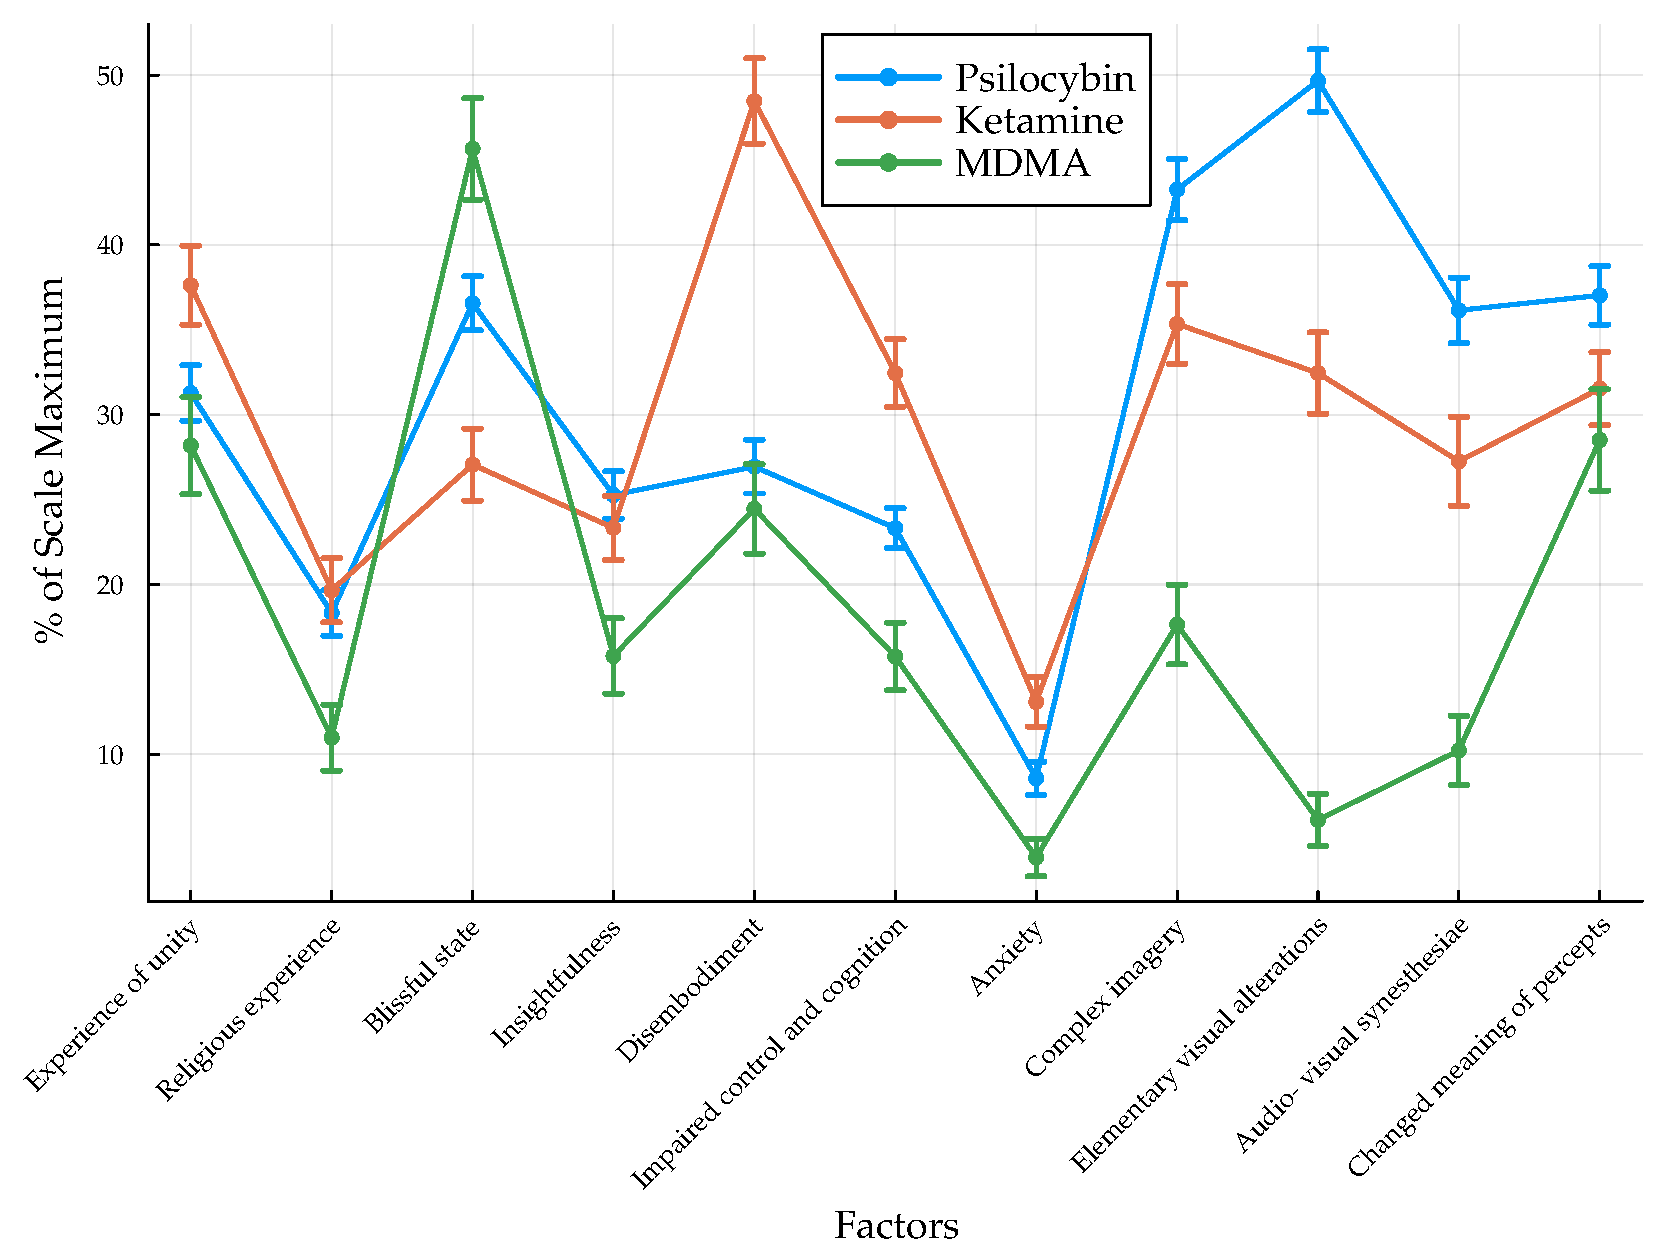
\includegraphics[width=\textwidth]{oavvalidationfigure2data/effects_plot.pdf}
  \caption{MDMA, ketamine, and psilocybin's effects on consciousness, as measured by the new OAV factors developed by \textcite{studerus2010psychometric}. Error bars represent standard errors. Figure re-plotted from the data underlying the original Figure 2.}
  \label{consciousEffects}
\end{figure}
\FloatBarrier

\subsection{Dosing}
\label{sec:dosing}
Accurate dosing is important for avoiding unnecessary side effects and optimizing effectiveness. The effects of MDMA primarily depend on dose, body mass, and, to a much lesser extent, how active your CYP2D6 enzymes are (they metabolize the MDMA)~\cite{studerusResponse}.

MDMA therapy only works within a certain range of doses. A dose of 0.75\,mg/kg, for instance, doesn't provide any significant increase in the effects commonly associated with therapeutic benefit~\cite{bediMDMALowDose}. We have also seen multiple anecdotes that too high of a dose can cause the session to be so blissful that you aren't able to productively engage with and reconsolidate maladaptive schemas.

The two primary risks of higher doses are oxidative damage in the serotonin system and long-term cognitive impairment~\cite{baggottDamage}. We discuss these further in Medical Risks. The first has been measured in animal experiments but hasn't yet been clearly linked to any clinically relevant impacts. The latter has most clearly been seen only in recreational users who use lots of MDMA over long periods of time in relatively unsafe contexts. It's not clear how relevant either are for less frequent, moderate doses in MDMA therapy.

This section describes two sets of dosing recommendations for different individual circumstances and risk tolerances, along with our recommendations. We've pieced this together from sparse data, meaning that, unfortunately, different parts report fixed doses vs. mg/kg doses. Session frequency, another important piece of safety, is addressed separately in \cref{frequency}.

\paragraph{The First Set} These doses are more conservative and based on a body of evidence suggesting that these doses do not cause measurable oxidative damage in the serotonin system~\cite{baggottSupplements}.

\textcite{liechtiInteractions} recommends a standard single dose of 100\,mg for body mass less than 60\,kg (132\,lb) and 125\,mg for higher body mass, though up to 200\,mg can be used for the highest body masses\footnote{M. Liechti, personal communication, December 11, 2025, clarified that 200\,mg is the maximum total dose, not a maximum initial dose. It also only applies to individuals with higher body masses, though specifics weren't mentioned.}. The 100\,mg dose also applies to everyone over 75\,years old. This is roughly equivalent to the 2\,mg/kg maximum recommended by \textcite{baggottSupplements}.

CYP2D6 poor metabolizers have stronger reactions to MDMA~\cite{schmid2016cyp2d6}. People who happen to know they have this should use up to a 25\% lower dose, though it's not essential~\cite{liechtiInteractions}. Various drugs, like bupropion, also affect dose.

Adjusting the dose in subsequent sessions might be necessary to match the effect of the medicine to the strength of your schemas or to deal with avoidance or tonic/collapsed immobility. The peak plasma concentration and likely total oxidative stress increase significantly faster than linearly above 125\,mg in the $>$60\,kg group~\cite{de2000nonlinear}. For instance, increasing from 125\,mg to 150\,mg doubles the peak concentration. For the $<$60\,kg group, this faster increase presumably starts at a lower dose; we speculate 100\,mg based on initial dose recommendations \todo{Is this a reasonable speculation?}. Therefore, we suggest increasing or decreasing your dose in smaller increments than you would expect when you're above the initial doses recommended by \textcite{liechtiInteractions}. We think a 10--15\% increase or decrease per session when above the standard dose is reasonable \todo{Is this reasonable?}.

Accurate data on the upper limit of safe doses is unfortunately absent due to difficulties translating the results of animal testing to humans and confounding factors muddying the study of harmful effects in recreational use~\cite{passieHistory}.

\paragraph{The Second Set} These doses have been successfully used in large clinical trials without any obvious, lasting adverse effects~\cite{mithoeferSafety}, but there is lower certainty that they do not cause small amounts of oxidative damage or cognitive impact.

Two sessions using a total fixed dose of 188\,mg did not cause any statistically significant, lasting cognitive issues in one clinical trial~\cite{mithoeferSafety}. This was used as the basis for the large phase III trials that used three 180\,mg sessions~\cite{mitchellMDMAClinicalTrial}. One-third of that total dose came from a booster dose 50\% the strength of the initial dose taken 1.5--2.5\,hours later to extend the productive duration of the session~\cite{mitchellMDMAClinicalTrial}. They did not measure oxidative damage.

Because effects depend on body weight~\cite{studerusResponse}, we don't recommend the fixed dosing these trials used. Adding a 50\% strength booster dose to the first set of recommendations from \textcite{liechtiInteractions} is a better option for those using booster doses.

\paragraph{Our Recommendations} We think the higher dose recommendations are a fine starting point. A handful of therapeutic sessions is not likely to have significant negative effect, and the mental health benefits can be large~\cite{mitchellMDMAClinicalTrial2,mitchellMDMAClinicalTrial}. Longer-term high-dose use may also occasionally be worthwhile for individuals for whom lower doses and other therapeutic modalities do not work well.

As a general principle for everyone planning more than a handful of sessions at the higher total doses, we strongly recommend finding your minimum effective dose. First, establish an effective MDMA therapy routine and gain a good sense of how your sessions feel and produce durable therapeutic improvement. Then you might reduce your total dose by 10\% each session until you notice sessions becoming slightly less helpful. Judge this a few weeks after the session, after the afterglow is finished and you have stabilized to a new baseline. This small reduction is unlikely to waste a valuable session by making it completely ineffective. You can also always return to your previous dose in the current session with an additional booster of the right dose.

The reductions can be done by reducing both the initial and booster doses by 10\%, or by eliminating the booster dose and increasing the initial dose such that the total dose is reduced by 10\%. In our experience, the single initial dose often provides enough working time to get us to the therapy hangover limit. If therapy hangover is the limiting factor, then a higher dose may not add much benefit\footnote{It's conceivable that a booster dose could push someone through their single-dose therapy hangover limit, but that would also result in even higher levels of post-session therapy hangover if it's possible.}.

There are a few other preventative measures for oxidative stress that some people use. Most of these have not been tested in humans, and therefore the dose and practical utility are unclear. We recommend primarily focusing on reducing your MDMA dose in the face of these uncertainties, though people doing a number of higher-dose sessions could consider trying some of these.
\begin{itemize}
    \item \textbf{Caffeine:} High doses of caffeine exacerbate neurotoxicity in rats given large doses of MDMA~\cite{vanattouCaffeine}. We think the precautionary principle is sufficient to warrant caution. Withdrawal is also undesirable, so it may be worthwhile to taper off moderate-high doses of caffeine for the months--years of MDMA therapy.
    \item \textbf{Warm Ambient Temperature:} High ambient temperature exacerbates neurotoxicity in rats given large doses of MDMA~\cite{baggottDamage}. It may be prudent to avoid hot ambient temperatures during sessions. It's plausible that the combination of high temperatures and high humidity is even worse given that it reduces the cooling effect of sweating.
    \item \textbf{Antioxidants:} High doses of certain antioxidants, including alpha-lipoic acid, ascorbic acid (vitamin C), and acetyl-L-carnitine, prevent oxidative stress in rats given extremely high doses of MDMA~\cite{aguirre1999alpha,shankaran2001ascorbic,alves2009acetyl}. See \textcite{baggottSupplements} for more information.
    \item \textbf{SSRIs:} Fluoxetine and likely other SSRIs taken 3--4 hours after the MDMA prevent neurotoxicity in rats~\cite{baggottDamage}.
\end{itemize}

\subsection{When to Seek Emergency Care}
Most of the interactions that cause severe acute harm are known and can be avoided with proper precautions or by avoiding using MDMA~\cite{riggDeaths,malcolmSerotonin}. However, individuals may not always follow proper precautions or may have undiagnosed health conditions. The direct causes of severe acute damage involving MDMA are almost always high body temperature, hyponatremia, or serotonin syndrome~\cite{riggDeaths,malcolmSerotonin}. Cardiovascular events may also rarely occur, especially when MDMA is combined with other drugs associated with cardiac function abnormalities~\cite{makunts2023concomitant}.

Many typical symptoms of heat illness, hyponatremia, serotonin syndrome, and cardiac events are also therapeutically appropriate symptoms of MDMA, fight-or-flight, freeze, tonic/collapsed immobility, and confronting extreme fear or anger. Thus, MDMA-therapy-specific recommendations are important. \textcite{malcolmER} recommends seeking emergency care for any of these symptoms of serotonin syndrome: myoclonic seizures, fever greater than 38.5\,°C (101.3\,°F), fluctuating or unstable blood pressure and heart rate, delirium or coma, and muscle rigidity. As far as we can tell, that recommendation also covers severe hyponatremia, which is only possible with very high fluid consumption, and severe non-serotonin-syndrome heat illness \todo{Do you agree? I haven't been able to find any reasonable hyponatremia guidelines that distinguish from normal MDMA therapy symptoms.}. In the absence of MDMA-specific advice, the cardiologist Nicole Bhave, MD offers this general advice for what type of chest pain you should go to the emergency room for~\cite{chestPain}: \todo{Do you know of any better advice?}
\begin{quotation}
    \dots it most often boils down to the severity of the pain and the heart attack symptoms we mentioned above. If the pain is so severe that you feel like you can't function, or if you are experiencing central or left-sided chest pain---especially if you have nausea or a cold and clammy feeling [also side effects of MDMA~\cite{liechtiGender}] alongside it---it is always safest to go to the emergency room. With chest pain, it's best to be cautious.
\end{quotation}

\subsection{Drug Interactions}
MDMA has dangerous or undesirable interactions with various drugs, supplements, and herbs. If you regularly take another drug, we suggest consulting \textcite{liechtiInteractions,spiritMemberProgram} (more accessible) or \textcite{sarparastDrugInteractions} (more technical) for recommendations on whether you should continue or discontinue it during MDMA therapy, avoid MDMA, or modify the MDMA dose. If your medicine is essential for your health, we strongly recommend consulting your doctor or pharmacist for help managing this. They will likely not understand the effects of MDMA, so you may need to provide \textcite{sarparastDrugInteractions} to them. That paper discusses pharmacokinetics, pharmacodynamics, and psychiatric drug interactions.

If you can't access a doctor or pharmacist, pausing a drug for 3 half-lives\footnote{One half-life is the time it takes for a drug's concentration in your body to decrease by half. Each drug has a different half-life, which can be found on \href{https://go.drugbank.com}{DrugBank} under Pharmacology → Metabolism. So the concentration would be 50\% after one half-life, 25\% after two, etc.} before the MDMA dose and 24\,hours (3 MDMA half-lives) after might work, provided a few conditions are met. The drug shouldn't be critical for your health, isn't one of the few high-risk interactions discussed in the section summary, and can be paused safely and with tolerable effects. This doesn't work as well for drugs whose effects persist after the drug itself has been flushed out. Certain health conditions also affect half-lives.

Most supplements and herbs can just be paused on treatment day to be safe.

In this section we list a couple of classes of interaction, then the most risky specific interactions and a few other selected interactions that frequently appear in therapeutic contexts. Combining MDMA with other prescription psychiatric or psychoactive drugs causes various changes to the intensity or duration of different effects, including changes to the efficacy of MDMA therapy~\cite{sarparastDrugInteractions}.

\paragraph{The most risky classes of interactions:}
\begin{itemize}
    \item \textbf{Serotonin Syndrome:} Serotonin syndrome is a potentially deadly condition caused by extreme amounts of intrasynaptic serotonin~\cite{malcolmSerotonin,sarparastDrugInteractions}. It's generally caused by interactions between MDMA and MAOIs or severe MDMA overdose.
    \item \textbf{Alterations in the CYP450 Enzymes:} The liver enzymes CYP2D6, CYP1A2, CYP2B6, CYP2C19, CYP3A4 (collectively called CYP450), and COMT metabolize MDMA and its metabolites (other molecules that the body converts MDMA into)~\cite{sarparastDrugInteractions}. drugs that enhance these enzymes may reduce the intensity and duration of MDMA effects by removing it from your blood at a faster rate. drugs that inhibit these enzymes cause higher and longer blood concentrations, though the multiple enzymes provide redundancy if one pathway is blocked. drugs that strongly inhibit multiple of these enzymes may be deadly to take with MDMA. drugs that only inhibit CYP2D6 are ok to take with MDMA, though \textcite{liechtiInteractions} recommends reducing the MDMA dose by up to 25\%.

    MDMA almost completely inhibits one of its own metabolic enzymes, CYP2D6~\cite{omathunaCYP}. This inhibition returns to baseline with a half-life of 47\,hours. Thus, about 2\,days after a session, enzyme activity will be 50\% of the way to baseline, 75\% after 4\,days, 88\% after 6, 94\% after 8, and 97\% after 10. This effect may counteract tolerance or lead to unexpectedly strong reactions to subsequent doses of MDMA. Inhibited CYP2D6 slows the metabolism of MDMA and many other drugs, especially ones that are not metabolized through any other parallel pathways that could take up the slack. Thus, dangerous concentrations of certain drugs could accumulate in your blood when those drugs are used within a few days after MDMA.

    \textcite{flockartTable} maintains a list of drugs that inhibit, enhance, or are metabolized by (called substrates) CYP450 enzymes.
\end{itemize}

\paragraph{Specific drug interactions, starting with the most risky:} (does not include low--moderate risk interactions with various drugs)
\begin{itemize}
    \item \textbf{MAOIs:} Taking irreversible MAOIs within two weeks before an MDMA session or within a few days after can cause severe serotonin toxicity and death~\cite{malcolmSerotonin,edinoffInteractions}. Ayahuasca contains a shorter-lasting, reversible MAOI whose effects are gone within 2--3\,days~\cite{malcolmAyahuasca}.
    \item \textbf{Ritonavir and cobicistat:} These strongly inhibit multiple CYP450 enzymes and can cause death~\cite{bracchi2015antiretrovirals,sarparastDrugInteractions}.
    \item \textbf{SSRIs and SNRIs:} SSRIs and SNRIs highly inhibit the effects of MDMA~\cite{feducciaSSRIDiscontinuation} but are not dangerous. Long-term use of these drugs causes this effect to persist long after drug discontinuation. The therapeutic efficacy of MDMA therapy is reduced by half even after 25\,days of discontinuation. Further discontinuation may bring further benefits. Discontinuation typically requires multiple additional weeks of tapering to manage withdrawal. See \prosecite{crossingZero} and \prosecite{malcolmTapering} for more information and practical advice on tapering.
    \item \textbf{Caffeine:} Large doses of caffeine \enquote{profoundly} increase tachycardia and body temperature in rats given large doses of MDMA~\cite{vanattouCaffeine}. It also increases the risk of serotonergic neurotoxicity to an unclear degree. It's not clear how this applies to human MDMA therapy, but caution might be warranted.
\end{itemize}

\subsection{Medical Risks}
MDMA's interactions with certain serious health conditions is not well understood. As of 2025, MAPS clinical trial exclusion criteria are commonly regarded as the baseline for what medical conditions are incompatible with MDMA. However, clinical trial exclusion criteria are conservative and designed to reduce unknown variables, regulatory scrutiny, and actual, if uncertain, harm. We think the exclusion criteria indicate that additional caution should be taken but are not all absolute contraindications. In the trials, \enquote{\dots any medical condition that could make receiving a sympathomimetic drug harmful due to increased blood pressure and heart rate \dots} was cause for exclusion, along with additional details for cardiovascular conditions discussed below~\cite{mitchellMDMAClinicalTrial2}. Please consult your doctor if there is any question about whether that applies to you. It would be useful to review the MAPS pharmaceutical investigator's brochure (\textcite{mapsInvestigatorBrochure})\todo{This document is too long to really be of use but I don't know what else to recommend.} with your doctor.

The trial inclusion criteria did regard some serious medical conditions as compatible with MDMA therapy~\cite{mitchellMDMAClinicalTrial2}. \enquote{Individuals with medical conditions such as hypertension, asymptomatic hepatitis C virus, diabetes mellitus, hyperthyroidism, and glaucoma were eligible, providing the condition was well managed and mild.} They couldn't have assessed every type of serious medical condition, so some conditions not on that list are presumably also compatible with MDMA therapy.

\paragraph{Preexisting health conditions:}
\begin{itemize}
    \item \textbf{Cardiovascular Disease:} MDMA increases blood pressure and heart rate, largely between hours 0.75--4 when a single dose is used~\cite{studerus2010psychometric}. Doses of 120\,mg + 60\,mg given roughly 2\,hours later increase average blood pressure by 28/12\,mmHg and heart rate by 23\,b/min over placebo in therapeutic contexts~\cite{mitchellMDMAClinicalTrial}\footnote{Averaged values from the 2nd and 3rd sessions. We excluded the 1st session because it used a different dose.}. This may be a risk for individuals with cardiovascular disease. Individuals with \enquote{\dots uncontrolled hypertension, history of arrhythmia\footnote{We suspect this doesn't include benign premature ventricular or atrial contractions since \~,50\% of people have them but haven't been able to confirm this.}, or marked baseline prolongation of QT or QTc interval} were excluded from clinical trials for this reason~\cite{mitchellMDMAClinicalTrial2}. \textcite{mapsInvestigatorBrochure} also states that \enquote{\dots any medical condition that could make receiving a sympathomimetic drug harmful due to increased blood pressure and heart rate \dots} was cause for exclusion. It's unclear exactly how much of a risk these actually pose, and clinical trial exclusion criteria are conservative. A search of the FDA Adverse Event Reporting System revealed, \enquote{A total of 17 unique cases were reviewed in this study. There were no reports where MDMA was taken as a single agent and ischemic, hypertensive, or arrhythmic adverse events were reported. All cases included co-use with other drugs associated with cardiac function abnormalities}~\cite{makunts2023concomitant}.

    People with anything more significant than \enquote{well managed and mild} cardiovascular illness, as assessed by a physician, might want to make precautions in case there is a problem during the session.
    \item \textbf{Liver Disease:} In one case, an individual with advanced alcohol-induced liver cirrhosis tolerated 100\,mg without issue~\cite{krausCirrhosis}. It's unclear how this generalizes to other cases and what the boundaries of safety are. Approach with caution with medical support.
    \item \textbf{Untreated Hyperthyroidism:} Rats with untreated hyperthyroidism given MDMA have a much higher risk of dangerously high body temperature~\cite{shokryHyperthyroidism}. Individuals with hyperthyroidism were allowed in the clinical trials provided that the condition was \enquote{well-managed and mild}~\cite{mitchellMDMAClinicalTrial2}.
\end{itemize}

\paragraph{Acute adverse effects:}
\begin{itemize}
    \item \textbf{Hyponatremia:} MDMA commonly causes mild hyponatremia (low plasma sodium concentration) in individuals who drink fluids as desired during the session~\cite{atilaHyponatremia}. We extrapolated from \textcite{baggottWater} that drinking a maximum of 0.5\,L of water during the six-hour session would easily prevent hyponatremia. It is also more than sufficient for preventing dehydration in the average person at a comfortable temperature~\cite{valtinWater}. Adding electrolytes has not been tested as a solution and is known to not prevent hyponatremia in athletic activities~\cite{hew2008statement}. People worried about dehydration could fully hydrate two hours before taking MDMA (Matthew Baggott, personal communication, November 24, 2025). That would provide enough time for the body to excrete any excess water by the time the session starts.

    On rare occasion, people at raves drink an extreme amount of water and die~\cite{riggDeaths}.
    \item \textbf{Heat Illness:} Prolonged, intense physical activity in high temperatures combined with dehydration can cause dangerous heat illness, as sometimes occurs at raves~\cite{vanOverheatingAlcohol}. Alcohol co-use significantly exacerbates this risk.
    \item \textbf{Seizures:} As with most problems associated with MDMA~\cite{riggDeaths}, seizures are very rarely reported. When they are, they are mostly associated with mixing intoxicants, extremely high doses, hyponatremia from drinking too much water, or heat stroke from dancing all night without adequate fluid intake~\cite{freidelSeizures}. It's possible that caffeine co-use could increase the risk~\cite{vanattouCaffeine}.
\end{itemize}

\paragraph{Chronic adverse effects:}
\begin{itemize}
    \item \textbf{Valvular Heart Disease:} Extremely high lifetime use of MDMA and possibly most psychedelics causes valvular heart disease via serotonin 5-$HT_{2B}$ receptor activation in heart valves~\cite{droogmans2007valvular,tagen2023valvular}. In one observational study, 28\% of chronic MDMA users showed signs of valvular heart disease (VHD) when evaluated with echocardiography, compared to 0\% in a matched control group who reported no MDMA use~\cite{droogmans2007valvular}. The chronic users with clinically significant VHD self-reported a mean consumption of 943 ± 1162 MDMA tablets, while the chronic users without clinically significant VHD reported a mean consumption of 242 ± 212 tablets. These results are so imprecise and assuredly confounded by abuse of multiple other drugs that they are inadequate as safety guidelines. Unfortunately, it's the only data we know of. We arbitrarily took half the lower number as a \enquote{don't exceed} limit.
    \item \textbf{Oxidative Damage:} MDMA causes oxidative damage in the serotonin system when the oxidative load of MDMA's effects exceeds the system's antioxidant buffer capacity~\cite{baggottDamage}. \textcite{baggottSupplements} states that there is decent experimental evidence that doses below 2\,mg/kg don't cause oxidative damage. Indicators of oxidative damage haven't been investigated at higher doses in humans.
    
    A dose of MDMA that is not neurotoxic in a single administration can also become neurotoxic when additional administrations are done before the antioxidant system has recovered~\cite{baggottDamage}. Unfortunately, it's not known how long this recovery takes. It's also unclear whether oxidative damage has any clinically relevant effects in the pattern of use used in MDMA therapy.
    \item \textbf{Long-Term Cognitive Impairment:} There is limited and contested evidence that many high-dose sessions cause long-term cognitive impairment~\cite{baggottDamage}. Unfortunately, it's unclear what counts as high-dose or what the shape of the session-count--impairment curve looks like. The evidence for this comes from a combination of observing inconsistent and mild behavioral differences after giving rats and monkeys extreme doses of MDMA and observational studies of recreational MDMA users. The human observational studies show an association between cognitive impairment and frequent or high cumulative use in recreational contexts. However, those studies rarely adequately control for the fact that recreational MDMA users often use a wide variety of other somewhat dangerous drugs (often mixed), overdose, or overheat or get hyponatremia at raves. One of the best observational studies, \textcite{corayMemory}, narrowed down the association to MDMA in particular, rather than other drugs the users had been taking. However, even that study did not control for the other mentioned factors that are not present in therapeutic contexts. One small randomized study of MDMA therapy did not find any significant cognitive effects after two sessions spaced 3--5 weeks apart using up to 188\,mg, but that doesn't rule out cognitive effects from a much larger number of sessions~\cite{mithoeferSafety}.
\end{itemize}

\paragraph{Higher risk groups:}
\begin{itemize}
    \item \textbf{Adolescents:} \textcite{kangaslampiAdolescent} saw no obvious reasons why adolescent use would be risky. However, this assumption has not been tested in any trials. Developing individuals could react differently to MDMA than adults.
    \item \textbf{Pregnancy:} There isn't any high-quality data about humans using MDMA while pregnant. The precautionary principle indicates that it should be avoided until it's rigorously demonstrated to be safe.
    \item \textbf{Lactation:} There isn't any high-quality data about humans using MDMA while lactating. The precautionary principle indicates that milk shouldn't be used while it contains significant amounts of MDMA. \textcite{bartuLactation} recommends discarding all milk from the 48-hour period following the use of methamphetamine. Its structural similarity to MDMA and longer half-life might indicate a useful recommendation for MDMA.
\end{itemize}

\subsection{Psychological Risks}
There is uncertainty about which psychological disorders are compatible with MDMA therapy. These are the exclusion criteria for the phase III trials~\cite{mitchellMDMAClinicalTrial2}:
\begin{quotation}
    Individuals were ineligible to enroll if they were unable to give informed consent. Individuals were also excluded for a history of or current primary psychotic disorder, bipolar I disorder, dissociative identity disorder, eating disorder with active purging, major depressive disorder with psychotic features, personality disorders, severe alcohol or cannabis use disorder (also moderate if not in remission), any substance use disorder other than cannabis or alcohol within 12\,months prior to enrollment \dots [or] serious imminent suicide risk \dots
\end{quotation}

Clinical trial exclusion criteria are conservative and designed to reduce unknown variables, regulatory scrutiny, and actual, if uncertain, harm. We don't know their reasoning for each item, but have some informed speculation. MDMA therapy induces psychotic episodes on rare occasion, though risk is likely higher in those with a personal history. Amphetamines are a known risk factor for manic episodes. Personality disorders make forming a healthy relationship between a client and therapist difficult to achieve. MDMA therapy might produce overwhelming destabilization in people with dissociative identity disorder if it facilitates abrupt confrontation of extremely distressing dissociated schemas. The trial environment and staff were likely not equipped to cope with some of these conditions, even if they might be addressable with MDMA therapy.

Mental illness treatment is highly individualized. Therefore, we don't think most of these conditions are necessarily absolute contraindications. Rather, each case should be assessed on an individual basis for its expected reward/risk ratio. Individual practitioners have different capacities for which symptoms they can support in their clients. Client factors include the amount of destabilization they can cope with at a particular point in their life, how capable they are at managing dysregulation, how much their basic functionality depends avoiding certain feelings or memories, and how much healthy external support they have.

We know that some people have enough resources, skill, and slack to use solo MDMA therapy to successfully treat debilitating mental illness. Many more people can use solo MDMA therapy to reconsolidate relatively minor issues. Skilled, ethical, and well-matched professional support is especially desirable for people with significant risk factors for dangerous conditions like suicide, psychosis, and mania. However, we recognize that people sometimes have to make the best of bad situations. Solo MDMA with risk factors might occasionally be a better option than the available alternatives, though this is highly individualized and we can't make any specific recommendations.

Professionals should be able to accurately identify each of the following conditions and have a plan to either manage them or get the client to an appropriate higher level of care. We rank these according to our impression of risk, starting from the most significant. See \cref{sectionManagement} for management recommendations and when and where to seek additional care.
\begin{itemize}
    \item \textbf{Destabilization:} Psychological destabilization (see \cref{sec:complex}) is a common occurrence in therapy~\cite{olthofDestabilization}. It's associated with better outcomes later in therapy, but if it is intense enough and not managed well, it can severely interfere with your life.

    We think it's likely that MDMA therapy tends to produce stronger destabilization and more rapid therapeutic progress than traditional psychotherapy. Severe trauma, diagnosis of mental illness, and severely disorganized attachment are risk factors. People are sometimes not explicitly aware they have gone through severe trauma. This may happen if the trauma takes the form of disorganized attachment, abuse is explained away as cultural tradition or \enquote{how things are,} the trauma took place in the period of childhood amnesia, or it is not remembered for another reason. The therapeutic alliance (see \textcite{BRWAIdownload} for an assessment scale) is a moderate mitigating factor when working with a mental health professional~\cite{fluckiger2018alliance}.

    We haven't been able to find any data on destabilization specific to MDMA therapy. The next best data we know of, \textcite{evans2023extended}, surveyed people who experienced new, persistent negative symptoms after recreational, professional-therapeutic, and DIY-therapeutic psychedelic experiences. This data applies to all psychedelics, not just MDMA, and a significant part of it only applies to traumatic experiences caused by large doses of hallucinogens like LSD, ayahuasca, or psilocybin. Most symptoms dissipated with time, but 17\% of respondents said theirs lasted more than 3\,years. From most to least common, participants reported emotional (76\%), self-perception (58\%), cognitive (52\%), social (52\%), ontological (50\%), spiritual (34\%), perceptual (26\%), and other (21\%) difficulties. These symptoms could be due to~\cite{calder2025traumatic}
    \begin{itemize}
        \item surfacing of existing maladaptive schemas and subsequent defense cascade activation, a necessary and healthy part of the therapeutic process if managed well. You may have been avoiding these schemas until the session. \textit{We think there is a high likelihood of this for MDMA therapy. It's conceivable that a skilled MDMA therapist could help you keep destabilization to small, easily dealt with chunks, but altered states of consciousness are difficult to control.}
        \item trauma from life impairment or destabilization due to poorly managed surfacing of maladaptive schemas and trauma. \textit{This happens, though the risk can probably be reduced with assistance from a skilled, ethical, and well-matched (see \textcite{BRWAIdownload}) mental health professional}~\cite{mdmaExtendedEvans,fluckiger2018alliance}.
        \item trauma from the psychedelic experience itself. \textit{We think this usually results from large doses of hallucinogens, unsafe settings, and abusive or incompetent guides/therapists. Traumatization risk may be low for MDMA itself because of its intense feelings of safety and low hallucinatory and mystical effect}~\cite{studerus2010psychometric}.
        \item difficult or destabilizing changes to your understanding of self, existence, or meaning. \textit{We think this is uncommon compared to psychedelics since MDMA produces minimal ego-dissolution and mystical experiences; however, it does happen}~\cite{ingramMDMA,martinInsight,holze2020distinct}. See \cref{selfinsight} for more information.
        \item something else. We don't know if this exists, and if it does, what it is or how often it occurs.
    \end{itemize}

    Even in this subgroup of people who have experienced extended difficulties in the previously mentioned study, 90\% agreed with the statement \enquote{I believe that the insights and healing gained from psychedelics, when taken in a supportive setting, are worth the risks involved}~\cite{evans2023extended}. However, it is possible that a population of psychedelic users who experience debilitating effects was missed due to sampling bias.
    \item \textbf{Psychosis:} \label{psychosis} There is virtually no high-quality experimental data because people with a personal (though not family) history of psychosis were excluded from clinical trials~\cite{mitchellMDMAClinicalTrial2}. Like other mental illnesses, psychosis is a complex biopsychosocial phenomenon. Therapy often reduces the symptoms of psychosis~\cite{CBTp}, suggesting that maladaptive schemas often play some role, though how strong that is compared to other factors likely varies by case. This implies that psychosis can start and stop at hard-to-predict points during the reconsolidation process and in life in general for people with some level of predisposition.

    We've seen a collection of anecdotes congruent with this complex framing~\cite{goodmanPsychosis,redditPsychosis1,redditPsychosis2}: A few self-reports from people stating that a single MDMA therapy session triggered a psychotic episode. Four reports from people stating that an MDMA therapy session resolved an existing psychotic episode. A few cases where people have safely used MDMA therapy despite previous psychosis, even when psychedelics were major causes of the psychotic episodes.

    Psychosis may be difficult to predict, but there are well-known risk factors. High doses and frequent use of a wide range of psychoactive drugs (especially cannabis) are well-established risk factors~\cite{drugsPsychosis}, as is stress~\cite{winkelPsychosisStress}. This explains why case reports of MDMA-induced psychosis typically, though not always, report confounding factors like co-use with other psychoactive drugs, chronic abuse of other drugs, heat stroke, hyponatremia, extreme doses, or extreme frequency of use~\cite{psychosisTreatment,arnovitzSchizophrenia,mcguirePsychosis,patelPsychosis,vaivaPsychosis}. We have also heard two anecdotes congruent with this multi-factor risk. In both cases, high-dose psilocybin trips conducted the day after an MDMA therapy session caused psychotic episodes.

    Substance-induced psychosis sometimes transitions into schizophrenia, but it's not known how likely this is in responsible MDMA therapy withough abuse of multiple drugs.

    MDMA-induced psychosis is definitely a risk for those with a predisposition, but some people with risk factors may still think it's worth trying. There are some precautions people with a history of psychosis should take if they try MDMA therapy. You could minimize the known risk factors of stress~\cite{winkelPsychosisStress}, cannabis~\cite{drugsPsychosis}, and abrupt withdrawal of antipsychotics~\cite{moncrieffAntiPsychotics} and GABAergic sedatives (e.g., alcohol, benzodiazepines). Skipping the booster dose of MDMA might also help, assuming a dose-dependent risk.
    \item \textbf{Suicidal Ideation and Behavior:} MDMA therapy with high levels of support decreases suicidal ideation on average about as much as placebo with the same level of support~\cite{mitchellMDMAClinicalTrial,mitchellMDMAClinicalTrial2}. When interpreting these results, it is important to understand that average improvements can mask the possibility that a small portion of individuals can get worse while the majority improve. Of course, though this applies to the placebo group as much as the MDMA group. Suicidal ideation is part of the biopsychosocial complex system of mental health. The psycho/schema component seems particularly influential since suicidal ideation almost always involves accompanying schema-like beliefs and justifications. Suicidality might get worse for a period of time, like many other schemas during the reconsolidation process.
    \item \textbf{Mania:} There is virtually no high-quality experimental data because people with bipolar I were excluded from clinical trials~\cite{mitchellMDMAClinicalTrial2}. The MDMA phase III trials did not exclude individuals with bipolar II, and no manic episodes were reported. Bipolar I might be excluded because psychological stress, sleep disruption, and dopaminergic amphetamines are linked to mania~\cite{salvadoreMania}, though MDMA releases much less dopamine than other amphetamines~\cite{kankaanpÄÄDopamine}. Bipolar I frequently also involves psychosis, which does have a link to MDMA use.

    Puzzlingly, we couldn't find a single published case report of mania where MDMA was unambiguously involved in the recent past. We only found two plausible self-reports of MDMA-induced mania on the Internet that didn't obviously involve major confounding factors not present in therapeutic contexts~\cite{erowidMania1,erowidMania2}\footnote{We searched for the terms \enquote{manic} and \enquote{mania} on reddit.com/r/mdma, reddit.com/r/mdmatherapy, and erowid.org and read every result.}. One individual with preexisting bipolar II claimed that MDMA triggered a manic episode. The other individual claimed that MDMA consistently triggered manic episodes; it's unclear when their bipolar disorder started and they were using higher doses of MDMA than is used in therapy. Only two reports is notably different from MDMA-induced psychosis, where many case reports are easily found.

    While commonly regarded as risky, actual risk in therapeutic contexts is unclear. There are some precautions that people with a history of mania should take if they try MDMA therapy. Adequate pre- and post-session sleep is critical given sleep's role in mania. MDMA should be taken early in the morning so that it's easier to sleep that night. It would also help to have a short course of sleep aids supplied in advance in case there are post-session sleep issues. High doses of caffeine might be avoided on the day of the session and continue until short-term side effects have dissipated~\cite{laraCaffeine}, though abrupt withdrawal would also increase risk. Skipping the booster dose of MDMA might also help, assuming a dose-dependent risk.
    \item \textbf{Addiction:}
    A panel of drug misuse experts assessed recreational MDMA as having among the lowest risk of dependence---\enquote{a propensity or urge to continue to use despite adverse consequences}---and harm among 20 of the most popular illegal or harmful drugs~\cite{nuttDrugHarms}. Alcohol, tobacco, and cannabis all scored far worse. Withdrawal has also not been found in rodent studies, even at extreme dosing schedules~\cite{robledoDependence}. When MDMA is abused, it seems associated with partying or avoidance of difficult feelings rather than therapeutic engagement~\cite{erowidAbuse}.

    Context is a critical component of addictive potential. Many commonly abused prescription drugs do not cause addiction or harm when used appropriately. The same panel scored several classes of prescription drugs, including amphetamines (some ADHD drugs), benzodiazepines (short-acting anti-anxiety drugs), ketamine, and opioids (painkillers), as far more harmful than MDMA in recreational contexts~\cite{nuttDrugHarms}. This might indicate that, when used responsibly for therapy, MDMA also has a lower risk of dependence and harm than medical use of those prescription drugs. Congruent with this, no instances of MDMA dependence have been reported in clinical trials~\cite{colcott2024side}.

    This suggests that the addictive potential of MDMA therapy is minimal for most people. If you are particularly worried about your potential for addiction or have significantly impaired impulse control, we suggest only doing MDMA therapy in structured, professionally guided contexts. This might include people in remission from serious amphetamine or cocaine addictions who might find the effects of MDMA close enough to the effects of their abused drug\footnote{The addiction pharmacology of these substances might share enough similarities with MDMA to warrant caution~\cite{nutt2015dopamine}. Other classes of addictive substances have different addiction pathways.}.

    MDMA therapy has shown tentative promise for improving other addictions. Structured MDMA therapy with high levels of support was well tolerated in individuals with current mild alcohol addiction or early remission of moderate alcohol addiction and did not lead to increased alcohol intake~\cite{nicholasAlcohol}. People using MDMA therapy for recovery may be interested in \textcite{recoveryPsychedelics}, a 12-step program for integrating psychedelics into recovery.
    \item \textbf{Hallucinogen Persisting Perceptual Disorder:} Complex or compelling distortions of external reality on MDMA are rare and correlated with unusually high doses~\cite{liechtiGender}. People more commonly have closed-eye visuals, possibly involving traumatic events they experienced. These visuals may be symbolic instead of a realistic reliving. Temporary and mild visual changes such as color and texture enhancement are also common.

    Experiences involving a combination of intense fear and visual distortions, like some MDMA and psychedelic experiences, occasionally create the persistent visual distortions or anxiety about existing but unnoticed visual distortions~\cite{halpernHPPD}. When this causes significant distress or impairment, it is called Hallucinogen Persisting Perceptual Disorder (HPPD). HPPD is strongly, but not exclusively, linked to pre-existing anxiety or dissociative disorders and often improves as those are treated. HPPD from MDMA is unrecorded in clinical trials, but some recreational users report it~\cite{vizeliActuteEffects,litjensHPPD}. One survey found that when people do report persistent visual or auditory distortions (from MDMA or psychedelics), 73\% say \enquote{they [the symptoms] don't bother me at all,} 24\% \enquote{I'd rather not have them, but I can live with them,} 0\% \enquote{they irritate me,} and 1\% \enquote{they drive me mad}~\cite{carhart2010user}.

    Given its origin in the combination of fear and sensory perception, we think HPPD is likely one of many possible somatic symptoms of mental illness in the model of \textcite{berghPsychogenic} that we expand on in \cref{psychogenic}. In that model, the initial experience creates a link between visual distortions and fear. The resulting HPPD would be either fear-driven hyperfocus on normal visual distortions that are typically filtered out of awareness or fear-driven hyperfocus on abnormal visual distortions that the brain recreates as top-down sensory fudging. Either could be treated with reconsolidation, which is congruent with the finding from \textcite{halpernHPPD} that HPPD improves as the associated anxiety and dissociation are treated.
\end{itemize}

\subsection{DON'T EVALUATE Other Common Concerns}
\begin{itemize}
    \item \textbf{Loss of Control:}
        MDMA does not strongly impair control and cognition~\cite{studerus2010psychometric}. One panel of drug-misuse experts ranked MDMA at 2\% the risk of alcohol for \enquote{harm to others}~\cite{nuttDrugHarms}. While engagement with distressing feelings can be intense, people also regularly have clear, emotionally nuanced conversations on MDMA~\cite{colbertEvenings}.
    \item \textbf{Drug Stigma/Discomfort:}
        Many drugs\footnote{Technically, a drug is any substance that affects the body or mind. The term has come to also mean \textit{illegal drugs}.} are harmful; however, during the War on Drugs, a wide variety of psychoactive substances were further stigmatized and categorized as harmful without clear evidence-based distinctions regarding their actual risk~\cite{alexanderNewJimCrow,nuttDrugHarms}. There is little correlation between the legality of MDMA and its potential for harm. One panel of drug misuse experts categorized recreational MDMA as 13\% as harmful as alcohol, 35\% as harmful as tobacco, and 45\% as harmful as cannabis. That's even in recreational contexts where users likely aren't as careful as they could be. Additionally, most of that harm is attributed to certain avoidable interactions~\cite{riggDeaths}.

        MDMA therapy is not for everyone, but discomfort is not a barrier to MDMA-facilitated reconsolidation. It might help you process your fear of drugs.
    \item \textbf{Misuse:}
        We are not aware of any clear evidence indicating that recreational or solo-therapeutic use of MDMA is problematic as long as the safety considerations in this section are followed. One panel of drug-misuse experts estimated that MDMA poses a significantly lower overall health risk than marijuana and far less than alcohol~\cite{nuttDrugHarms}. While those drugs can be used in harmful ways, they can also be used responsibly with negligible negative effects. In recreational contexts it's still important to avoid mixing drugs (including alcohol), and additional precautions may need to be taken to offset sweating with more water consumption, but not so much as to get hyponatremia.
    \item \textbf{Association with MAPS and MDMA Being \enquote{Synthetic}:}
        MDMA (\cref{fig:mdma}) is generally made by making several modifications to the plant compounds safrole (\cref{fig:safrole}) or piperonal (\cref{fig:piperonal})~\cite{worldDrugReport,euMDMA}. When properly conducted, this process results in pure MDMA. Single-substance purity greatly improves the ability to produce accurate and safe doses. Refer to \textcite{ruggeriNatural} for a nuanced discussion of what \enquote{natural} means. For those concerned about the pharmaceutical industry: MDMA was first made in the early 20th century by Merck as an intermediate product with no recognized use itself~\cite{passieHistory}. The first known human use of MDMA was in the early 1970s as a legal alternative for MDA in recreational use. Its first use in therapy occurred in the late 1970s after the independent chemist Alexander T. Shulgin realized its therapeutic potential and introduced it to the therapist Leo Zeff, PhD. Zeff then used it with many clients and taught many therapists how to use it. Then, once it was made illegal, legal therapeutic use ended. Making it legal again would require enormous amounts of money to run proper FDA-approved clinical trials. No regular drug company was willing to do this because the original patent expired in the 1930s, and they wouldn't be able to recoup their investment through drug sales. The 21st-century clinical trials were funded through a combination of (a) donations to the nonprofit Multidisciplinary Association for Psychedelic Studies (MAPS) and (b) MAPS selling shares of its for-profit division Resilient Pharmaceuticals (formerly Lykos, formerly MAPS Public Benefit Corporation)~\cite{lykosPatents}. To recoup their investment, Resilient tried to patent a specific particle size of MDMA crystals within a pill, but the patent office rejected it. Their business plan is now unclear. As far as we are aware in 2025, outside rare clinical trials or limited legal use in certain countries, all MDMA used in therapy is ultimately sourced from underground chemistry labs and has nothing to do with Resilient or MAPS.
        \FloatBarrier
        \begin{figure}[htbp]
        \centering
        \chemfig{*6(-=-(--[::-60](-NH-[::-60])-[::-60])=-(*5(-O--O-))=)}
        \caption{Structure of MDMA.}
        \label{fig:mdma}

        \vspace{1em}

        \chemfig{*6(-=-(--[::-60]=[::60])=-(*5(-O--O-))=)}
        \caption{Structure of Safrole.}
        \label{fig:safrole}

        \vspace{1em}

        \chemfig{*6(-=-(-=[::-60]O)=-(*5(-O--O-))=)}
        \caption{Structure of Piperonal.}
        \label{fig:piperonal}
        \end{figure}
        \FloatBarrier
    \item \textbf{Unlearning Healthy Schemas:}
        \label{unlearnHealthy}
        As stated by \textcite{ecker2015misunderstood}:
        \begin{quotation}
            When two mutually contradictory schemas are juxtaposed consciously, the schema that more comprehensively or credibly models reality [including yourself], and therefore more usefully predicts how the world will behave, reveals the other schema to be false, and the falsified one is immediately transformed [reconsolidated] accordingly.
        \end{quotation}

        The reconsolidation process doesn't imply that your post-reconsolidation beliefs will be a precise truth about the world or yourself, only that they will be more true than the falsified/unlearned schema in the context of your lived experience. We think this generally produces good outcomes but is not perfect. There might be rare situations where a healthy but false-according-to-your-lived-experience schema is unlearned. For example, someone's especially deep desire to not be alive might be able to contradict their desire to, say, avoid falling off cliffs. In that case their avoid-falling-off-cliffs schema would be an unintegrated remnant from a time in their life when they did want to be alive. In case such a scenario is actually possible, please do not try to unlearn any schemas critical for keeping you or any other being safe. Do not conduct MDMA therapy in acutely dangerous situations where healthy danger avoidance schemas may activate. We also hope that using MDMA's compassion, connection, and safety to facilitate reconsolidation of your fears and insecurities also tends to result in schemas that are associated with more compassion, connection, and safety. On a practical level, we are unaware of any instances of MDMA therapy unlearning a fundamentally healthy schema. The closest example we are aware of is the unlearning of fear-based schemas that, while unhealthy, may temporarily provide some necessary functionality in your life (see \cref{sec:complex}).

        Similarly, the reconsolidation process can't always help you unlearn erroneous beliefs that were formed from unrepresentative sets of experiences. If you were the first human to meet aliens, and they attacked you, you might reasonably learn, \enquote{these aliens are dangerous.} No amount of reconsolidation will change that until you acquire contradictory knowledge, like learning that that alien was a pirate but all the other aliens are very nice people.
\end{itemize}

\section{Session Frequency and Scheduling}
\label{frequency}
Specific recommendations for session spacing are difficult because individuals have different risk/reward tradeoffs and physiological responses to MDMA. There are two main limitations important for minimizing risk~\cite{baggottSerotonin,baggottDamage}. First, the brain's antioxidant capacity needs time to replenish after a session. MDMA causes oxidative stress, but the brain's antioxidant buffer is normally capable of neutralizing this for the doses of MDMA recommended for therapy. However, using more MDMA before it has recovered will cause oxidative damage to the serotonin system\footnote{We don't think using antioxidant supplements to do more frequent sessions is wise because the oral dose of antioxidants humans need to prevent oxidative damage is unknown~\cite{baggottSupplements}. It's not even established that it's possible or safe to get plasma concentrations high enough using oral dosing. The studies demonstrating antioxidant protection injected rats with massive doses.}. There is no solid data on how long this takes. For lack of a better idea, the 6\,week spacing used in the phase III trials might be a decent minimum spacing.

Second, the serotonin system downregulates during an MDMA session, causing short-term tolerance~\cite{baggottSerotonin,baggottDamage}. Using MDMA again before tolerance has returned to baseline will result in lower efficacy, and using higher doses to overcome that will increase the risk of oxidative damage if the dose becomes too large for the antioxidant buffer to handle. Neither the time required for tolerance to return to baseline nor the limits of the antioxidant buffer are well known, so we strongly recommend spacing sessions far enough apart that you don't notice any lessening of effect.

Doing sessions more frequently than those limits may also risk long-term tolerance, called \enquote{losing the magic}~\cite{baggottSerotonin,baggottDamage}.

% We think the six-week spacing used in the phase III trials is a reasonable minimum session spacing, though longer is always ok too~\cite{mitchellMDMAClinicalTrial2}. From there, we recommend establishing an effective MDMA therapy routine and gaining a good sense of how your sessions feel and produce durable therapeutic improvement. Then, if you feel that a shorter spacing would benefit you, you might reduce your spacing by one week each session until you notice sessions becoming slightly less helpful. Judge this a few weeks after the session, after the afterglow is finished (see \cref{afterglow}) and you have stabilized to a new baseline. This small reduction is unlikely to waste a valuable session by making it completely ineffective.

% That procedure only measures short-term tolerance. You may \textit{not} be able to notice when you go below your antioxidant system recovery timespan. In the absence of better evidence, the previously mentioned 3--5 weeks might be a reasonable minimum. Where you fall in that range depends on your risk/reward balance.

See \prosecite{baggottSerotonin} for further discussion of tolerance and oxidative stress.

\paragraph{Additional Downsides of Frequent Sessions:}
\begin{itemize}
    \item More frequent medication pausing or tapering if your medication is incompatible with MDMA.
    \item People with risk factors for psychosis may want to avoid frequent sessions, since frequent use of a wide range of psychoactive drugs is another well-established risk factor for psychosis~\cite{drugsPsychosis}.
    \item Frequent sessions may be emotionally taxing.
\end{itemize}

\paragraph{Benefits of Frequent Sessions:}
\begin{itemize}
    \item \textcite{berghSelfEvidencing} hypothesizes that the high-level schemas predicting pervasive threat that many people with mental illness have can easily categorize minor negative stimuli as new threats\footnote{\prosecite{alexanderPrecision} provides a more accessible summary of the paper.}. This process can readily create new maladaptive schemas. Put another way, relatively minor events can easily traumatize people with mental illness. We speculate that this might show up in therapy as \enquote{two steps forward, one step back,} or needing to achieve some intensity of reconsolidation just to maintain baseline. Actual improvement would depend on higher intensities of reconsolidation.
    \item Similarly, from a complex systems approach, it's conceivable that certain complex maladaptive schema networks may reconstitute certain components over time after those components are partially or fully reconsolidated. High intensities of reconsolidation over short-to-long periods of time might be needed to reconsolidate multiple reinforcing components and break free of these traps.
    \item Another session after a few weeks might provide enough additional reconsolidation to resolve particularly overwhelming destabilization from a previous session that doesn't respond to other symptom management strategies.
    \item More frequent sessions probably deliver more therapeutic progress, especially if other methods don't work for you.
    \item Many people who might benefit from working with a skilled, ethical, and well-matched mental health professional can't access one because of maladaptive schemas related to interpersonal trust. Relatedly, many people already have a therapist but don't get much benefit out of therapy because of similar reasons. A critical mass of MDMA therapy sessions may provide a valuable on-ramp to greater amounts of therapeutic support and success. This can lead to a strong upward trajectory, whereas the same amount of reconsolidation spread over a longer period of time might not achieve the same critical mass necessary.
\end{itemize}

\paragraph{When to Schedule Sessions}
It may be especially productive to schedule sessions when you have a few hours of available time most days for the next 1--3 weeks. Some people report that reconsolidation exercises like therapy are more productive than normal in this period of afterglow (see \cref{afterglow}). Spending a few hours a day paying attention to the emotions that came up during the session may also be particularly useful (see \cref{increasingAttention} (Increasing Attention)). We list some ideas for when to schedule sessions in \cref{sessionDecision}.
\FloatBarrier
\begin{table}[htbp]
\caption{Example decision matrix for when to schedule MDMA therapy sessions, based on available time and session cost. This represents our informed thoughts and is not based on any rigorous research process. Individuals will need to consider other factors as well.}
\label{sessionDecision}
\centering
\begin{tabular}{|p{2.7cm}|p{6.15cm}|p{6.15cm}|}
    \hline
    & \centering\textbf{Low Session Cost} & \centering\textbf{High Session Cost} \tabularnewline
    \hline
    \centering\textbf{Lots of Time} &
    \centering Whenever you want. Experiment with different frequencies to see how they affect therapeutic progress. &
    \centering When you have enough time to max out on post-session reconsolidation every day. \tabularnewline
    \hline
    \centering\textbf{Little Time} &
    \centering Ideally, when you can make time for post-session reconsolidation, but sessions may still be very helpful without much post-session reconsolidation. &
    \centering When you can make the most time for post-session reconsolidation. \tabularnewline
    \hline
\end{tabular}
\end{table}
\FloatBarrier

\section{Professional Guidance vs. Self-Guidance}
\label{professionalVSSelf}
MDMA therapy can succeed in a wide variety of contexts, including therapist-guided sessions with pre- and post-session support, do-it-yourself couples therapy, and solo therapy~\cite{mitchellMDMAClinicalTrial2,colbertEvenings,hillsSolo}. However, we believe working completely alone with MDMA presents higher risks and a lower healing likelihood compared to partnering with an ethical, skilled, and well-matched mental health professional (see \cref{sec:howtofind} for definitions). However, that may not always be the best option available because it is often difficult and expensive to access an ethical, skilled, and well-matched therapist or guide. This is especially common for those who have had a series of negative experiences with mental health professionals. Per our individual and clinical experience, an ethical, skilled, and well-matched therapist or guide may provide
\begin{itemize}
    \item a trustworthy presence that creates a greater feeling of safety, enabling more effective healing
    \item additional perspective that's difficult to see from a first-person view
    \item education on trauma, healing, trust, what healthy relational patterns look like, and healthy ways to deal with emotions
    \item troubleshooting for problems with the medicine or other parts of the healing journey
    \item improved screening for conditions that might make MDMA particularly risky for an individual
    \item monitoring of your level of destabilization over time
    \writtenByDay{
    \item a skilled and experienced perspective about how best to maintain your window of tolerance and broaden it over time
    \item assistance in learning appropriate coping strategies
    \item assistance identifying which coping strategies are best for you in a particular context
    \item assistance preparing executive function supports for yourself to maximize your capacity to use the right strategies at the right times
    \item management of destabilization periods to reduce disruptions to your life, including empathetic encouragement to rest or cut back from other obligations when appropriate. This preserves overall wellness and capability.
    \item guidance through difficult therapeutic exercises
    \item an empathetic and grounding presence while you think through major life decisions, relational challenges, and challenging new schemas that may emerge in the course of the work
    \item assistance identifying supplementary treatment modalities that are likely to be most effective for your situation, and in some cases, information about how best to access those treatment modalities
    \item assistance in planning for your medicine experience and organizing appropriate social support for the whole process
    }
    \item unadulterated medicine or some degree of medical monitoring, depending on who you're working with
\end{itemize}

Therapists and guides who are ethical and skilled but whose style or personality are not a good match for you should be easy to approach about this mismatch. They might even recommend any colleagues who they think would be a better match. The risks inherent in working with an ethical and skilled therapist or guide who you don't match well with mostly involve wasted time and money, and possibly demoralization. However, the risks of unethical or unskilled therapists and guides can include
\begin{itemize}
    \item emotional, physical, financial, or sexual abuse. This includes Adverse Idealizing Transference (see \combinedcref{def:ait}).
    \item dependence
    \item increased risk of adverse effects and destabilization
    \item demoralizing, ineffective treatment
    \item false beliefs of abuse~\cite{Scoboria07022017} or false beliefs about how trauma and mental illness work
\end{itemize}

\label{suicideCops}
Licensed mental health providers are usually legally obligated to call the police on you if they think you are at high risk of imminent suicide, hurting someone, or are so psychotic that you might do one of the former accidentally~\cite{alexanderInpatient}. In practice, it depends on their interpretation of local laws that they may not understand, how much they fear being sued or losing their license if someone is hurt, and how much they believe involuntary hospitalization will help you. If you are suicidal or fantasize about hurting your abuser, we strongly suggest asking your provider to elaborate on their decision criteria before you open up to them. Then you can decide if you can cope with the level of self-censorship necessary to not cross their boundary. Or, you may trust your provider enough that you can be completely open with them because you know they will only tell you to go to the hospital if you really need it. In that case you could write up a crisis plan involving which hospital you want to go to, which family members or friends you want notified, etc. If your provider does call the police on you, know that police typically have little training in mental health and will likely take your provider's word over yours. There is also a good chance that the police dragging you away against your will to a place you can't leave---where medical staff may do various invasive and non-consensual things to you---will traumatize you. Even worse, \textcite{emanuelHospitalization} found that (at least in Allegheny County) involuntary hospitalization actually significantly increases the chance of a patient killing themselves or hurting someone else over the 6\,months following admittance in cases where clinicians might disagree about admitting a patient (43\% of evaluations in this study). It's not clear how well these results apply to situations where multiple clinicians would all agree on admitting a patient. \textcite{alexanderInpatient} is a good guide for navigating/avoiding the inpatient mental health system.

Individual and couples MDMA therapy without professional assistance appears to work well for some people, including the author M.G.~\cite{hillsSolo,colbertEvenings}. This may or may not include the assistance of a trusted, empathetic, and emotionally non-reactive sitter~\cite{thalSitter}. We are uncertain what circumstances lead to positive vs. negative experiences or the degree to which various risks are increased. We can't say if this is appropriate for your particular situation, but it is an option that many people like for various reasons. Scheduling is an obvious advantage; you don't need to find a day when your mental health professional is also available. Cost is also a huge advantage. In 2025, in the US a guided MDMA therapy session costs in the upper \$100s to \$1000s per session~\cite{sessionCost}. MDMA itself only costs 6 to 50\,Euros per gram (in Europe in 2022), which is enough for 5--10 sessions~\cite{euMDMA}. Solo use may also sometimes be a decent option for many people who have been traumatized by mental health professionals or who can't access a good one.

We propose the following ranking of options for people who can access a skilled, ethical, and well-matched mental health professional. The top of the list represents the lowest risk of adverse outcomes (largely destabilization), the highest likelihood of durable healing, and also the highest financial cost. The tradeoffs are different for those who have been traumatized by professionals or who cannot access the right professional help. In that situation the status quo of mental illness is an additional risk, and minimizing risk may occasionally mean doing solo sessions. This list is a general guide, and the exact positions of items are debatable, as well as dependent on personal circumstance. Exceptions to the rule always exist.
\begin{enumerate}
    \item Continually working with a skilled, ethical/accountable, MDMA-trained therapist or guide you align well with. \textit{This model is the only one that has been investigated in clinical trials, where it was shown to work well. We think this model is especially important for people with potentially dangerous symptoms they can't manage themselves, possibly including, but not limited to, psychosis, suicidal behavior, or a severe lack of impulse control.}
    \item Start off with a skilled, ethical/accountable therapist or guide who you align with and who is MDMA-trained or personally experienced with MDMA and many of the difficulties that can arise in MDMA therapy. You may later transition to self-guided sessions (with as-needed check-ins) if you and your clinician collaboratively decide that your reward/risk ratio is high enough. \textit{Some people pursue this method because it offers dramatically lower costs, and there are many anecdotes of people (including the author M.G.) who have found it highly effective.}
    \item Work with a skilled, ethical, accountable, non-MDMA-trained therapist or guide you align well with; collaboratively assess your risk factors with them. You might read the safety section of this guide together or consult a MDMA-trained therapist. If your reward/risk ratio is high enough, you then self-guide all your medicine sessions while maintaining as-needed sessions with your clinician. You also use high-quality resources (see \cref{sec:psychoeducation}) to educate yourself on the nuances of effective and safe MDMA therapy and use a high-quality sitter as appropriate, which includes at least the first several sessions (see \cref{def:sitter} for characteristics of good sitters). \textit{We think this model is somewhat more difficult and riskier than the previous option.}
    \item Self-guide all your medicine sessions and do all of your own between-session work, perhaps talking about your healing journey with emotionally skilled friends or friends skilled in safely using MDMA for healing. You also read high-quality literature (see \cref{sec:psychoeducation}) on trauma healing and use a trusted sitter for at least the first few sessions. \textit{We don't recommend this model for people who can access good professional assistance because self-assessment of risk factors is difficult. Not having an expert to discuss things with may make various parts of the process harder. It may be the best option for some people who don't want to or can't work with a professional and who have the capacity to manage intense and difficult emotional experiences.}
    \item Self-guide all your medicine sessions and do all of your own between-session work. You don't use any high-quality reference material and don't understand the nuances of safe and effective healing. Or you work with an incompetent or abusive guide or therapist who may harm you by suggesting overly intense MDMA sessions and not effectively help you with the resulting destabilization. They may also offer distorted or unhealthy interpretations of experiences you have during a session. \textit{We don't recommend this in any circumstance. While it is occasionally helpful to some, the lack of rigorous understanding of the process can place both safety and healing at elevated risk and is likely to impair healing to some degree. Adverse effects may not be identified, understood, and well managed.}
\end{enumerate}

Group therapy might offer lower cost but comes with a different set of risks and tradeoffs~\cite{marseille2023group}.

\section{How to Find a Therapist or Guide}
\label{sec:howtofind}
\textit{M.G.'s note:} \href{www.reddit.com/r/mdmatherapy}{/r/mdmatherapy} maintains a list of guide and therapist directories and referral services in the sidebar (on the new Reddit; not old.reddit.com). We have not vetted most of them. You may also be able to find guides and therapists by talking to people at psychedelic meetups. Also, in addition to the information in this section, \prosecite{safetyFlags} is a list of green/yellow/orange/red flags to look for in practitioners.

Which therapist you work with matters a lot. For instance, in a large study done by \textcite{firth2019therapistEffects}, after adjusting for demographic factors like symptom severity, the best 3.9\% of clinicians had 77.2\% of their clients recover; the recovery rate for therapists in the average range was 58\%; and the 3.9\% of clinicians who had the worst outcomes only saw 41.4\% of their clients recover. Note that a significant percentage of people recover even without therapy, so the worst therapists might have a negative influence on their clients.

It is our hope that the following recommendations, which largely emerge from our personal and clinical experience\footnote{This experience includes some common knowledge of professional norms among the licensed mental health professions, much of which can be found in the ethics codes of the major licensed mental health professions. These include codes of ethics from the National Association of Social Workers, American Psychological Association, American Counseling Association code of ethics, American Association for Marriage and Family Therapy, etc.}, can make finding a therapist less overwhelming and more hopeful for those who are struggling with the search.

First, we acknowledge the difficulty: even under optimal circumstances, accessing mental healthcare can turn out to be a slog. These challenges are common knowledge for people who provide community mental health services or who have accessed them repeatedly: the financial and administrative costs are often daunting. Interacting with licensed mental healthcare professionals is inherently vulnerable for many, especially those who have witnessed or experienced carceral hospitalization or forced medication. Intake interviews frequently demand intimate details of your finances, sexuality, and medical and mental health. All of this is the price of accessing a clinical relationship that may or may not be very helpful. If it isn't, clients may feel they need to stick with it because they do need help, and finding someone else to help them seems like more than they can take on. That doesn't necessarily mean the clinician will stick around, especially if they are students whose clinical internships end only a few months after starting to work together. Online services, which have endeavored to bridge the gap between what is needed and what is easily available, are plagued by serious ethical and product-quality concerns~\cite{betterhelp1,betterhelp2,betterhelp3,talkspace1,doneglobal1}.

The good news is that there \textit{are} excellent clinicians out there, and not all of them are late in their careers. Early career therapists, like those who tend to staff more affordable clinics, provide just as good of care as their more experienced counterparts~\cite{goldberg2016psychotherapists}. Here are our recommendations on how to find one that's right for you.

\subsection*{Bad Therapy is Worse than no Therapy}
Remember that really bad therapy can really hurt you~\cite{hook2018boundary}, and as such we feel it is worse than no therapy. Bad therapy can leave you stagnant for a long time with the impression that no real help for you exists. It can make your symptoms worse without subsequently improving them. In the worst scenario, it can leave you with additional trauma. See \combinedcref{sec:mdmaTherapistComplications} for a discussion of the particular challenges of avoiding negative and damaging clinical experiences in the realm of MDMA therapy.

Good therapy is often very uncomfortable~\cite{eckerUnlocking}. However, you should feel a sense of mutual trust, respect, collaboration, and consent regarding the goals you are working towards and the methods you use to get there~\cite{BRWAIdownload}. We think a skilled and well-matched clinician will take the time to help you develop trust commensurate with the discomfort of what they are asking you to undertake. They should do this even if you don't understand the methods your clinician is using to help you.

Although we cannot speak to the specific trade-offs of your situation, in general we recommend continuing to search until you can access good therapy.

\subsection*{Trust Your Personal Experience}
Trust your perceptions, because your personal experience of your clinician impacts the efficacy of your treatment~\cite{horvath2011alliance}. You don't just need a good provider, but a good provider who is also a good fit with you. We strongly recommend using the BR-WAI~\cite{BRWAIdownload}, an empirically validated tool for understanding how you and your therapist are connecting and what might be required to improve that connection.

In our experience, it's a good idea to look for someone it feels like you could say anything to. If you cut your arm, any skilled emergency physician will be able to competently stitch you up. The same is not true with a comparable degree of psychiatric injury~\cite{firth2019therapistEffects}. In mental healthcare, the bedside manner is part of the intervention, and the same bedside manner doesn't work for everyone. Although the most skilled mental healthcare providers connect well with an extremely broad spectrum of clients, it is unrealistic to expect every provider to \textit{click} with every client. Many excellent mental healthcare providers ultimately focus narrowly on particular populations of interest to them. If you aren't connecting with a particular clinician, it doesn't mean anything is wrong with them, and it doesn't mean anything is wrong with you.

\subsection*{Feedback}
Good therapists love feedback and direction. It is likely that many therapists who could do great work with you if you are expressive about what you need and want would, in contrast, be bad therapists for you if you aren't expressive about those things~\cite{macdonald2015correcting,delgadillo2022progress,lambert2001effects,oanes2015therapists}. If you can, we recommend asking clearly for what you want and talking clearly about how things feel. Additionally, there are several instruments that have been developed to help therapists measure and improve their performance. Examples include the BR-WAI, the ORS-SRS, the Core-OM, or the QR-45.2. If your therapist asks you to participate in one of these formal feedback mechanisms, we recommend doing so, even if it feels awkward. These measures really appear to help therapists provide better services.

We've observed that it is sometimes helpful to imagine what therapy would be like if it went as well as you could possibly imagine and to share this, and your fears about the process, with your clinician. You can also ask if your ideal hopes align with their experience of their methodology, which may help you set expectations for your treatment. You can use the list above (of what a skilled therapist can provide) to identify ways you would like your therapist to support you. It may be helpful to identify which forms of support you are interested in receiving and to spend some of your initial sessions learning how your clinician feels about providing support in those particular ways.

If you have been working with a particular clinician for a while and your issues are within their main practice area, you are \textit{well} within your rights to ask them to learn or implement a new-to-them intervention. An accredited therapist is required to complete continuing education hours anyway. There are many legitimate reasons they may say no, like cost, time, and accessibility of additional training, and that's OK too, but please don't be afraid to ask.

Sometimes things don't work out even after you've made some effort to recruit your clinician's help in fixing the situation. As a final service, they may be willing to spend some of your final few sessions helping you find and connect with someone who is a better fit.

\subsection*{Boundaries}
\label{def:ait}
Good therapists have good boundaries. Clients often come to therapy without an understanding of what healthy therapeutic boundaries are and why they might be important. That's OK; it is the clinician's job to have this knowledge, to share it with the client, and to assert boundaries as needed.

One of the most critical reasons boundaries are crucial in therapy is a phenomenon called adverse idealizing transference (AIT)~\cite{hook2018boundary,transferranceLoveHarm}. Idealizing transference is a phenomenon in which clients develop strong positive feelings towards their therapist. This can be totally healthy and extremely helpful to the course of therapy, supporting clients in their sense of safety and their ability to sustain focus and effort through the sometimes severe discomfort of healing. However, in some cases, it is possible for these positive feelings to be so strong and misdirected that they cause considerable harm, causing lasting distraction and disruption in the client's life, potentially continuing for decades. This situation creates a severe vulnerability that the therapist, if they are unscrupulous or unskilled, may exploit (intentionally or not) for emotional, sexual, or financial gain, creating severe trauma for the client and sometimes impacting others as well. In these cases, idealizing transference has become adverse idealizing transference. Just as helpful drugs sometimes have side effects for a small percentage of the people who use them, a small percentage of therapy consumers experience AIT.

AIT can happen even when a clinician is doing everything right~\cite{transferranceLoveHarm}. However, both the emotions of AIT and the harm created by them can be greatly amplified when therapists fail to communicate and follow through on healthy boundaries. Here are some commonly recognized healthy professional boundaries for therapists:
\begin{itemize}
    \item The clinician does not disclose details of their personal life to you unless that disclosure enhances your treatment and is motivated by a desire to promote your welfare.
    \item The clinician avoids dual relationships wherever possible. For example, if a client cannot pay for services and offers to do yard work or provide other professional services in barter, it would cause a dual relationship to accept this offer. The most commonly accepted exception to the dual relationship rule is in extremely rural practice, where access to services is very limited. For instance, a clinician might provide mental health services to someone who is also their children's pediatrician. However, in these cases, other professional boundaries should still be maintained on both sides.
    \item The clinician is very clear from the beginning of treatment about their policies. These include the location and timing of sessions, confidentiality practices, payment details, acceptable communication channels outside of therapy sessions, contact outside the therapy context, lateness, and missed sessions. The clinician follows through on these policies as stated and communicates any policy changes in a timely way.
    \item The clinician does not communicate to you in any way that they feel differently about you than they do about their other clients, or that they treat you differently than their other clients.
    \item The clinician does not permit or encourage the exchange/offering of significant gifts, especially financially significant gifts.
    \item The clinician does not provide advice outside the realm of their expertise; most clinicians minimize the time they spend giving advice even within their expertise, because supporting clients in the process of arriving at their own conclusions is more aligned with ethical standards and more effective towards lasting change.
    \item If physical touch is engaged in at all, it generally should be minimal, such as a brief hug at the end of each session or a single brief hug at the termination of treatment. Physical touch may be avoided entirely, and if present, must be for the client's benefit, not the clinician's.
    \item Even if the clinician is providing therapy on a very generous sliding scale basis that is essentially free for an individual with great financial need, it is a good sign if they insist on always charging a fee. A fee less than a dollar can still serve as a healthy reminder about the nature and boundaries of the relationship, helping both client and clinician maintain a mindset that minimizes the risk of AIT.
\end{itemize}

Therapists are, unfortunately, not explicitly educated on AIT at this time. We strongly recommend that all clinicians read the two reference articles for this section. That said, therapists in all the major licensure categories should be familiar with and generally compliant with the boundaries listed above; understanding the importance of boundaries and respecting the vulnerability of clients are important topics in their clinical training.

Per item 3 on this list, if you are a client with a high number of risk factors for AIT~\cite{transferranceLoveHarm,hook2018boundary}, we recommend discussing preventative measures with your clinician. You might also heavily weigh boundary practices in your assessment of clinicians' fit for you. Note that these risk factors are not required to develop AIT, nor do they guarantee AIT. They simply correlate with an increased risk. The risk factors include
\begin{itemize}
    \item a history of dependent/idealized relationships, especially with health professionals
    \item an approach to therapy that is primarily seeking care, rather than insight
    \item unrealistic views of what therapy can provide
    \item being female, especially if working with a male therapist who is older than you
    \item having a therapist of a gender you are sexually or romantically attracted to
    \item being a sexual minority
    \item experiencing significant symptoms on a spectrum with borderline or narcissistic personality disorder
\end{itemize}

A final recommendation on boundaries and the prevention of AIT: although confidentiality is a critical therapeutic boundary, we feel it is an excellent sign if your clinician seeks regular supervision and consultation as needed. They need to disclose some details to their supervisor or consultant, but it should only be the minimal amount necessary. Neither you nor your clinician should feel that anything is happening in the therapy room that they would be ashamed or embarrassed to disclose to a trusted friend in your case or a trusted HIPAA-compliant colleague in theirs. Therapy should feel private, but if it starts to feel like a secret, something may be off.

\subsection*{Targeted Therapy}
In our experience, in some circumstances it is important to seek therapy that is targeted to the challenges you are experiencing. One of the most common and arguably benign forms of bad therapy happens when clinicians offer a generally empathetic and supportive environment without bringing clients into a space of productive discomfort. This often results in therapy that feels pleasant but not very helpful and which perpetuates the damaging myth that working with a skilled mental healthcare provider is interchangeable with, but pricier than, having an empathetic friend.

Although the current diagnostic system is substantively flawed~\cite{cohen2023need,eaton2023review}, we recommend that a best practice for seeking effective mental healthcare is first obtaining one or more accurate diagnoses. Second, research the most evidence-supported treatments for your diagnoses. Then, seek clinicians who are trained and experienced with those specific treatments and ideally, who are experienced using those specific treatments to address those specific diagnoses. According to both our personal experience and Thomas Insel, MD~\cite{eksIncel}, this leads to radically better outcomes than a less targeted search for mental health treatment.

A less medicalized approach to this process recommended by a colleague~\cite{sinback} is to identify what kind of change you would like to make with the help of a professional. Then, do some research on how people seem to be working towards that change in various contexts and seek a professional who has a good reputation or training in that method. This may be especially appropriate if the help you are seeking is not specifically oriented around mental illness.

This whole sequence may or may not feel accessible to you. However, we recommend that if you are experiencing therapy that feels pleasant but not as helpful as you need it to be, it is worth discussing it with your therapist. You can ask what specific interventions and modalities they are employing and what might work better. Often, in this situation, you as a client require a treatment method that will push you more.

\subsection*{Finding a Therapist Can Be a Long-Term Project}
If you feel daunted by the process of finding a good therapist, we strongly encourage you to recruit some support and treat finding a therapist as a long-haul effort. For example, if you have a supportive friend or partner, you could ask them to commit to providing you with your favorite takeout every time you complete ten or fifteen \textit{actions} on your therapist search. These actions might include getting a list of clinicians your insurance covers, messaging therapists to see if they are taking clients, completing an intake interview, scheduling a session, and completing a session. Alternately, you might start a text thread with your closest supporters, where you can report your efforts and be rewarded with GIFs and emojis. A perspective shift that may be helpful when searching for a therapist is to regard each failure or action as an intermediate step towards finding the help you need and worth celebrating.

We recommend completing three or more sessions with a given therapist before committing to giving treatment with them a try. If you luck out and find a great fit on your first or second try, the BR-WAI will help you have confidence that you've really found what you're looking for. If a particular clinician (or a string of clinicians) is not a fit for you, that's OK too; that doesn't mean you have anything to apologize for. It's good to trust the process and expect that it may take some time.

\subsection*{Accreditation and Safety}
\label{sec:accreditation}
We would be remiss not to acknowledge that unlicensed\footnote{For the purposes of this section, when we say unlicensed, we are not referring to pre-professionals and pre-licensed professionals who are operating under the license of an independently licensed professional as part of their training progression. Examples would include a resident counselor or psychologist. In terms of accountability and ethics enforcement, we feel comfortable recommending this class of providers at the same level as independently licensed professionals.} or minimally accredited mental healthcare providers are common~\cite{aboujaoude2020coachingVSTherapy}, often billed as coaches, guides, shamans, pastors, or simply healers. In this era when a mass-scale mental health crisis is met with a healthcare affordability crisis in the USA, individuals in need of healing seek assistance wherever they can. Indeed, talk therapy and psychiatry are modern inventions, and we are aware both from common sense and through personal experience that skilled and ethical healers of mental and emotional distress exist across many contexts and training levels.

That said, it can be extremely difficult to verify whether the individual you are considering working with is ethical and skilled, and working with an unskilled or unethical provider can be extremely harmful~\cite{hook2018boundary,therapisttocoach}. Although the protection offered by working with a licensed counselor is imperfect, we feel it is a critical consideration, especially when working with MDMA, as described in \combinedcref{sec:mdmaTherapistComplications}.

We perceive significant risks associated with using an unlicensed mental healthcare provider. They may
\begin{itemize}
    \item provide, and charge for, interventions that are useless or harmful.
    \item not have been trained in differential diagnosis, and in any case are not legally permitted to diagnose you.
    \item provide services to you while they are impaired through the use of drugs or alcohol.
    \item not have received training about the importance of boundaries and of respecting the vulnerability of clients within the power dynamics of mental healthcare. If this is the case, they are less likely to express and enact boundaries and other practices that minimize the risk of adverse idealizing transference (AIT).
    \item enact harm that emerges not from the interventions themselves, but from other aspects of how they do business. For instance, unnecessary dual relationships or boundary violations can leave clients feeling disempowered, violated, or humiliated across multiple domains of their lives.
    \item encourage you, during particularly vulnerable and suggestible times, to make decisions that are bad for you and your life; they may leverage their intimate knowledge of your trauma to exploitatively encourage you to make choices that benefit them at your expense.
    \item not experience any negative consequences for physical, financial, or psychological harm that may come to you in their care. Exceptions might include crimes they commit in a way that would be recognizable as criminal and punishable by law even outside a therapeutic relationship.
\end{itemize}

The protections provided by working with a licensed professional are mediocre. For instance, the field of mental health talk therapy is still relatively young, and it is widely accepted that talk therapy is as much art as science. We have observed that most fully licensed professionals center their practices on interventions that could be covered by insurance, and this may provide some probabilistic guardrails against interventions that have no empirical support at all. However, even among fully licensed practitioners, there is little enforcement that compels clinicians to focus on the most empirically validated interventions or delivery methods. There is also little enforcement for matching a client's particular situation to the most empirically validated treatment for that specific situation. If these practices are important to you, we recommend asking many detailed questions about them when you are searching for a well-matched therapist.

Additionally, we have observed that various systems of power and oppression can and do play out in the therapy room if clinicians are not actively, vulnerably, and skillfully working to avoid this outcome. The prestige and respect generally afforded to therapists can sometimes foster hierarchical and non-collaborative dynamics. Therapists sometimes say extremely inappropriate, dismissive, harmful, or stigmatizing things. That can be even more harmful than normal because those statements were made by a therapist, someone who they perceive to be an expert and who is supposed to have the answers. Licensure does little or nothing to protect against or prevent these forms of harm.

Although cultural acceptance is improving, mental illness is still very stigmatized, and there are many reports of clinicians who turn on their clients, abusively labeling them \enquote{borderline} or simply crazy if those clients file a complaint against them~\cite{hook2018boundary}. The privacy of the therapy room, the power of stigmatized diagnoses, and the prestige of the therapist role mean that in \enquote{he said, she said} adjudications, a client is unlikely to be listened to. The situation is further complicated by the reality that clinicians really are misrepresented and attacked occasionally~\cite{gutheil1991patients,williams2000victimized}. This can emerge out of clients' profound attachment wounds, overwhelming trauma, and at times delusions, hallucinations, and paranoia. It is inherently very difficult to tell from the outside, and sometimes from the inside too, what has really gone on. As such, many therapists may be more likely to empathize with their peers~\cite{hook2018boundary} than wronged clients when they hear about misconduct by colleagues. This unfortunately creates a robust haven for a minority of unethical clinicians\footnote{\enquote{Studies generally show remarkable consistency in age, gender, and practice characteristics in that the typical transgressor [of sexual relationships with clients] is a middle-aged male therapist in solo private practice who engages in a sexual dual relationship with one female patient}~\cite{sexViolations}.}, extremely incompetent, negligent, or predatory.

Despite these shortcomings, we feel it is important to highlight the advantages of working with a licensed clinician and encourage you to weigh the risks carefully. Some certificates for coaching or Christian counseling can be obtained in a few weeks to a month for less than a thousand dollars. These kinds of certifications do not bring significant professional accountability. The loss of such a certification doesn't usually create significant occupational impairment, and certifications this small are not typically backed up by a licensure organization with sufficient resources to keep track of practitioner misconduct or enforce consequences~\cite{carr2015end}. Obtaining independent licensure as a mental health clinician demands years of study, additional years of supervision, and an often six-figure financial investment in education and accreditation. If a fully licensed professional practices therapy while they are impaired, crosses sexual boundaries with a client, or exploits clients for financial gain, the client can file a complaint with the clinician's licensure board~\cite{vinson1987complaintProcedures,barsky2023licensing}. If the clinician is then found to have committed the harm described in the complaint, they may, depending on their particular license and jurisdiction
\begin{itemize}
    \item have their name published on a state registry that lists the misconduct they were found guilty of
    \item be required to take ethics classes or complete other professional development work
    \item be required to work under a supervisor for a period of time, and during that time announce to every single client at the start of treatment that they are working under the license of another professional and who that professional is
    \item lose their access to providing treatment through a hospital they had previously worked through, or they may lose the ability to have their work reimbursed through insurance
    \item have their license entirely revoked for severe or protracted misconduct or if they refuse to comply with rehabilitation requirements
\end{itemize}

Independently licensed clinicians must typically pass a criminal background check to become accredited~\cite{dunlap2021background}. They may also lose their accreditation if they are found guilty of fraud, sexual misconduct, or abuse in other areas of their lives~\cite{barsky2023licensing}. This is an important safeguard because a pattern of exploitation across various domains of their life is one of the earmarks of a genuinely predatory individual, rather than simply incompetent~\cite{cooke2001refining}. These consequences are not always commensurate with the harm caused, but at least one study indicated that the process of filing a board complaint against a harmful clinician tends to be a positive experience for survivors~\cite{vinson1987complaintProcedures}.

To check whether your clinician is licensed or accredited in some way, try asking them for their license number and then looking it up on the website of their professional association. There are also several professional directories (e.g., Psychology Today in the United States) that will only list clinicians after verifying their credentials. In the United States, there are \textit{many} qualifications and certifications that allow a practitioner to legally provide mental health counseling. \todo{For a listing of the more common possibilities and a brief discussion of the differences between them, see Appendix NUMBER.}

To further add to the confusion, we have observed that even within the same license, training can vary widely. If you are committed to working with a licensed professional, we recommend searching for providers based on the professional's experience, preferred client demographic, or treatment modalities, and then verifying their license. You can attain a clearer understanding of the details of a particular clinician's background with the particular issues you are having or the particular modalities and interventions you are interested in being treated with by asking them detailed questions. For example, how many clients have you worked with who have x diagnosis? What is your training and background in y intervention? They might answer with details including trainings or continuing education units they have completed, books they have read, classes that were part of their degree, relevant experience with those populations before they became a therapist, and much more. All these details are highly variable between individual practitioners, but the baseline safety protections that come from working with a licensed professional are always attached to the specific license they hold. Finally, please note that the fields of life coaching, guiding, or other unlicensed professional support often serve as havens for individuals who have lost a license due to misconduct.

If you choose to work with unlicensed professionals, we recommend exclusively working with professionals who are very clear about their scope of care, participate in accountability and transparency practices like accountability pods\footnote{Accountability pods are a practice developed by the Bay Area Transformative Justice Collective. See \textcite{podmapping}.} and publicly post their business ethics (as exemplified in \textcite{sinbackValues}). Indeed, we feel these practices, though imperfect, are a green flag from providers of any licensure level. We hope they will become normalized across mental healthcare, along with providers routinely seeking appropriate supervision and consultation and being transparent with clients about who is supervising or consulting with them. Finally, many of the suggestions from \cref{individualActions} may be adapted to reduce your risk profile, even if you are not working with MDMA. The caveats we placed on that list apply here as well. No matter who you work with, if they choose to harm you through their behavior, that is not your fault.

To understand the scope of care when you are considering working with an unlicensed professional, it may help to ask detailed questions about which services they provide and how and where they learned the skills to provide those services. Unlicensed professionals are forbidden by law from diagnosing or treating mental illness~\cite{aboujaoude2020coachingVSTherapy,healthyGamerCoaching}. However, many of the interventions that are used to treat mental illness can be appropriately implemented by unlicensed professionals and have many legitimate uses outside mental illness treatment. For instance, some coaches teach reconsolidation, thought records, mindfulness practices (see \textcite{rain}), or myriad other skills and strategies that constitute legitimate mental illness interventions. These skills are not exclusively relevant to mental illness; a reasonable person might learn them simply to enrich their life and increase their personal growth. When unlicensed professionals deploy them, they are also not doing so (or legally should not be doing so) in the context of a treatment plan wherein a therapeutic relationship is constructed and interventions are performed that will specifically address a specific mental illness. As such, it can reasonably fall within the domain of unlicensed care to teach these skills and to help folks identify some circumstances where it is helpful to use them. These kinds of services may significantly help you self-manage or self-treat your mental illness, especially (as is often the case) if you are unable to access high-quality licensed mental healthcare.

On top of this, we've observed that unlicensed professionals are frequently helpful for bridging a gap between the needs of people with mental illness and the necessary level of support (often, more than meeting with a clinician once a week) that would allow them to achieve a significantly better quality of life. For example, a coach might call you several times a week when you are most vulnerable, to help you accomplish task initiation or avoid doom-scrolling, a service a therapist is unlikely to provide. Unlicensed professionals might help you with more practical, seemingly superficial, yet crucial aspects of changing your life for the better: sitting with you while you fill out job applications, or declutter your house, or practice eating mindfully. Some unlicensed professionals can help you learn and apply healthy relationship skills that will radically improve your life. Some carry out structured and empirically validated approaches and work under the supervision and organizational support of fully licensed professionals, as exemplified by the Healthy Gamer coaching programs~\cite{healthyGamerMethodology}.

In contrast, we believe the very best mental health professionals can complete a detailed biopsychosocial assessment of your situation, accurately diagnose you, and offer you mental health interventions that are well-suited to you. They offer a deep understanding of how various constellations of symptoms tend to show up and some awareness of pitfalls you are likely to encounter along the way based on that. They will have an understanding of what level of care is appropriate to your situation, and if they do not have the particular expertise appropriate to your condition, they will help you find a provider who does. They may know much sooner than you do if it is urgently important for you to receive a higher level of care. For instance, early intervention for a first psychotic episode has a massively positive impact on the lifelong trajectory of individuals with psychotic spectrum disorders, and timely intensive treatment for eating disorders or substance use disorders can be lifesaving. Particularly if you do not have a case manager to take on this role, a mental health professional may help you work through what is stopping you and learn the skills to recruit and coordinate care from many sources. Examples include
\begin{itemize}
    \item psychiatric prescribers
    \item specialist care providers like a dietitian or a trauma-informed OB-GYN
    \item peer support from friends and loved ones
    \item peer support from potential future friends and loved ones, as when joining an activity group that helps you stay consistent with positive coping strategies
    \item community programs, like a senior center, meditation center, or gym
    \item coaches, ecclesiastical leaders, or other appropriate unlicensed professionals
    \item personal care assistants to assist with the activities of daily living, when appropriate
\end{itemize}

Although reconsolidation may ultimately heal most or all of your mental illness in a deep and durable way, meanwhile you must live with your symptoms and build the best life you can, despite your symptoms. The best mental healthcare providers are experts not only in addressing the root causes of mental illness but also in helping you reduce the incidence of your symptoms and in helping reduce the impact of your symptoms on your life.

\subsection*{MDMA-Specific Complications in Obtaining Professional Care}
\label{sec:mdmaTherapistComplications}
Finding professional support for MDMA therapy carries challenges over and above the challenges of finding mainstream mental healthcare~\cite{patientVulnerability}. The specific nature of MDMA therapy amplifies the vulnerability of seeking psychiatric care, including (we surmise) vulnerability to AITs. Some of these challenges emerge from the legal status of MDMA therapy. Finally, these factors have combined to create an existing culture of underground MDMA therapy that can be painfully exploitative~\cite{powerTrip}. An effective process for securing professional support must take all of these challenges into account.

\subsubsection*{Challenges caused by the vulnerability of seeking psychiatric care}
As discussed in \combinedcref{sec:accreditation}, there is a severe power imbalance between providers and consumers of mental healthcare. When a fully licensed professional enacts behavior that is clearly abusive, it creates the case in which we would expect the maximum possible structural support for accountability within conventional criminal-legal and administrative systems. However, even in these cases, proving misconduct and enforcing appropriate consequences for it is not always possible~\cite{biaggio1998obstacles}. On top of this, we've observed that many individuals consuming mental health care feel that they must put up with a certain degree of discomfort to access care they may desperately need. We find they are often understandably unskilled at detecting the difference between the healthy discomfort of effective treatment~\cite{eckerUnlocking} and discomfort related to mistreatment or misconduct.

\subsubsection*{Challenges caused by the nature of MDMA}
As detailed below, MDMA can increase client vulnerability. MDMA can create experiences of great mental and sometimes physical intensity, of much longer duration than a traditional therapy session. Long sessions, sometimes a risk factor or \enquote{red flag} for harmful boundary violations~\cite{strom1999boundryViolations}, are necessary in MDMA therapy. MDMA can generate sexual feelings~\cite{mcelrath2005sex}, and we think the same enhanced empathy and openness to experience that make them such a fantastic aid to reconsolidation work may mean they leave individuals who take them more susceptible to persuasion. Altered states of consciousness also impair the ability to be appropriately cautious and thoughtful about risk. These factors make it even harder for clients to tell when providers are behaving inappropriately. Additionally, a significant subset of MDMA clients are having one of the peak experiences of their life, or even \textit{the} peak experience of their life. We think this could cause therapists and guides who routinely facilitate this therapy to feel godlike. Even excellent guides and clinicians may need to work very hard, when administering MDMA-assisted therapy, to maintain appropriate boundaries, humility, and client-centered care. This dynamic can undermine even good clinicians' ability to provide quality care. \todo{CITATION Matthew Johnson Summit talk}. Although there is no data on the topic, we feel this dynamic almost certainly increases the risk of AITs with MDMA therapy, particularly with providers who are not scrupulous regarding boundaries or thoughtful about preventing this specific risk. All of these aspects of MDMA amplify the already formidable power dynamics between a therapist and a client, regardless of legal status or other factors.

\subsubsection*{Challenges caused by legal status}
The legal status of MDMA creates additional risk for those seeking professional support for Psychedelic-assisted therapy (PAT) in several ways:
\begin{itemize}
    \item Mental health providers' training and experience around MDMA has been extremely limited by their legal status. This includes the ability of professionals to experience MDMA as a part of their training, which most clients and clinicians feel improves clinicians' ability to provide MDMA therapy and which many feel is essential to that ability~\cite{liknaitzkyProfessionalExperience}. However, clinicians generally cannot legally access these experiences with solid supervisory support. If clinicians even disclose their history of MDMA use, they could theoretically face some degree of legal or licensure-related repercussions. Even if the actual risk of repercussions is very low, the perceived risk may be high enough to prevent clinicians from becoming involved in these activities.
    \item The fact that everything has to be underground makes it harder for people to find each other as needed. \todo{The whole legal status section needs expert reviewer or citation help.} This can create a sense of scarcity, as in, \enquote{I have found a provider and need to stick to them because searching for a better fit feels daunting or impossible.}
    \item When the medicine is criminalized, clients who are harmed in therapeutic processes related to the medicine often legitimately fear legal or social consequences to themselves if they report crimes against them that were undertaken during this process. This makes the power dynamics astronomical.
\end{itemize}

\subsubsection{Existing culture of exploitation in psychedelic therapy}
Taken together, the above factors render it unsurprising that exploitation, spiritual bypass, and cultic dynamics seem to have been woven into the culture of underground psychedelic therapy~\cite{abuseLetter,brown2020ethical}. MDMA facilitates suggestibility and profound experiences. Providers face challenges in staying humble and client-centered when providing these interventions and have deep shelter from any legal threat about malpractice that is created when it is all illegal. These all play a role in a culture of guides, healers, shamans, and therapists who can harm with impunity. Multiple accounts have surfaced of the need to develop a better framework of accountability in these underground, unregulated communities.

If you are interested in learning more about this topic, we recommend the following resources:
\begin{itemize}
    \item \prosecite{abuseLetter}
    \item \prosecite{brown2020ethical}
\end{itemize}

\subsection*{Individual Actions to Improve Safety of MDMA Care}
\label{individualActions}
In this era of regulation, many people with mental illness are driven to work with unlicensed providers due to mistrust of the mainstream mental health system or the financial or logistical inaccessibility of high-quality licensed care~\cite{aboujaoude2020coachingVSTherapy}. Additionally, while the system of licensed providers presumably prevents many of the most egregious violations, some serious harm can and does slip through, as evidenced by the whistleblower reports from the MAPS trials~\cite{icerReport}. In this context, we believe there are steps some individuals may be able to take to increase their safety when seeking MDMA therapies.

We want to emphasize that even if you do nothing on this list, any care provider who violates the sacred trust you have put in them as a healer by mistreating you is fully responsible for their actions. Those who are most badly in need of psychiatric care are often under-resourced and likely to find it challenging or impossible to carry out the degree of vetting or preparation they might have ideally preferred. We are not providing these suggestions to cast blame or create additional responsibilities for care-seekers, but as a resource with which those who are able may be able to improve the risk profile of their healing endeavors.

\subsection*{License and Certification}
Research their license and certifications carefully. See \combinedcref{sec:accreditation} about accreditation and the protections it provides. Remember that practitioners may claim a license they don't have, or they may have some sort of certification that does not carry enough weight in their professional life to enforce any kind of accountability. We particularly recommend taking other precautions if your clinician does not belong to a licensing body that publishes the names of clinicians who are found to have violated its ethical code.

\subsection*{Evaluate Fit}
Follow the advice above (see \cref{sec:howtofind}) about finding a clinician who is a good fit for you, including working with them for at least three sessions (preferably five or more) before making any decisions about using their assistance for medicine work. During this time, observe their boundaries carefully, and have frank discussions about their qualifications, your needs and expectations, and the modalities that would be employed during the medicine work.

\subsection*{Methodology and Expertise}
Research their therapeutic methodology and expertise. \todo{Disclaimer that the research in conventional therapy does not support sorting by methodology. Also have this section reviewed by a sex therapist.} It is our hope that the evidence-based theoretical framework offered in this book, positing that the primary mode of healing MDMA offers is memory reconsolidation, can assist some clients in assessing whether they are interested in engaging with various therapeutic methodologies. Accordingly, we particularly recommend seeking clinicians who have a strong background in addressing immobility and panic, in dealing with trauma generally, and in assisting their clients in working through somatic manifestations of trauma/somatic release.

Although they may be particularly effective for activating some important schemas, we strongly recommend avoiding methodologies that involve physical touch, \textit{particularly} those that involve physical touch during the actual medicine work. The client may be unable to consent or make unbiased decisions about whether to continue or stop a particular therapeutic interaction in this state.

If you are interested in somatic methodologies that involve touch, we recommend alternatives such as therapeutic use of restorative yoga postures. In this practice, a clinician can provide support through various bolsters and pillows, along with verbal instruction, so that there is never any need to touch you in any significant way. If for some reason you do choose to pursue a methodology that involves touch, we recommend undertaking precautions to increase your sense of volition and improve the safety of the endeavor, including
\begin{itemize}
    \item creating a detailed written consent contract in advance of your medicine session that determines what forms of touch will be acceptable under what circumstances and how these boundaries will be upheld
    \item using witnesses and cameras to provide you with certainty that your wishes have been respected
\end{itemize}

We agree with the assertion of the American Association of Sex Educators, Counselors, and Therapists when they suggest that there is no circumstance where sexual touch is appropriate to the therapeutic relationship~\cite{aasectTouch}.

\textit{M.G.'s note:} Clients sometimes feel that therapy helped them remember traumatic events they weren't previously aware of~\cite{psychedelicrecoveredmemory}. These may or may not be accurate recollections of historic events, and we are not aware of any reliable method of distinguishing a memory's accuracy other than independent corroboration. To avoid incorrect interpretation of perceptions during the session, therapists and guides should categorically avoid suggesting a memory is either true or false and shouldn't even suggest that a specific individual has avoided memories they can recover~\cite{otgaarMemory}\footnote{People who retract claims of recovering accurate memories of abuse overwhelmingly blame their therapist for improperly influencing them~\cite{otgaarMemory}.}.

\subsection*{Background Check}
Get a background check on the guide and possibly on others who recommend them or who have trained them. In some cases, significant networks of recommenders or well-regarded trainers may all be invested in unsubstantiated or potentially harmful therapeutic modalities~\cite{powerTrip}. Historically, lineage of training has been an important way that healers are credentialed in the absence of licensure systems; if your guide has trained under someone who promotes potentially harmful therapeutic modalities, with concepts such as \enquote{breaking down} the client or helping them \enquote{fight it out,} or if they have been mentored by people who have a history of boundary violations against clients, we recommend proceeding with extreme caution if at all. If a guide with these red flags seems like an otherwise excellent match, we recommend having detailed conversations about how they relate to those practices and approaches, and taking the other safety considerations listed here especially seriously. Finally, as noted in the accreditation section, if a prospective professional support has a history of fraud or abuse in other areas of their life, this is also worth taking into consideration, even though it may appear unrelated, because this may be a warning sign for truly predatory behavior. \todo{Cite}

\subsection*{Accountability}
Look for external accountability in the clinician's ethical structure, both philosophically and practically. One of the concerns cited by \textcite{powerTrip} regarding safety in PAT is that there seems to be a cultural norm in underground psychedelic therapy of identifying the truth-including the truth about situations in which clients allege their clinicians have harmed them-as something that comes from inside each person. In contrast, healthy accountability practices require us to listen with openness to outside information which can make us feel downright terrible on the inside. We recommend seeking providers who maintain active relationships with supervisors, mentors, or accountability pods~\cite{podmapping} who can help them receive the report appropriately if a client has a bad experience in their care. Additionally, we recommend seeking clinicians who can provide you with a clearly articulated set of written ethical standards they endeavor to adhere to, whether those standards come from a professional organization or personal soul-searching.

\subsection*{Flight Plan}
Create a \enquote{flight plan} and a safety plan collaboratively with your provider/s while sober, and review/update it before each medicine experience. Birth plans have become popular tool that birthing parents can use to (a) educate themselves about the many choices that may emerge during labor and delivery, and (b) communicate strategically with providers about their needs and preferences; we feel that structured advance planning for PAT sessions could provide similar benefits~\cite{birthPlan}. Here are some considerations you may wish to include in your flight plan if you feel you are at particularly high risk for AIT (link to assessment questions in section above), or otherwise have significant safety concerns:
\begin{itemize}
    \item You may wish to have one or more support people present to serve as witnesses during your medicine session.
    \item You may even choose to delegate, \enquote{medical power of attorney} style, to allow trusted support people to make certain choices on your behalf while you are incapacitated by the medicine. If you pursue this possibility, it is important to have in-depth conversations with your support person and your clinician about what level of distress is appropriate for you to face, and what the likely outcomes of that distress may be-as well as having detailed discussions on the choices they are being entrusted to make. \todo{WHAT CHOICES MIGHT YOU DELEGATE?-also have this concept reviewed by an experienced psychedelic practitioner}
    \item You may wish to arrange to have your session filmed, possibly even from a few angles, so that you have a lot of concrete evidence afterward about what happened.
\end{itemize}

See \cref{prep} section for more information on flight planning. \todo{WE SHOULD TALK IN DETAIL SOMEWHERE ABOUT WHAT DECISIONS ARE REASONABLE TO DELEGATE OR NOT}

\subsection*{Cultishness}
Keep an eye out for cultic group structures or dynamics. Accounts from the underground PAT world have described closed systems centered around charismatic leaders, exploitation of the labor of group members, and abundant use of what cult scholars call \textit{thought terminating clichés}~\cite{powerTrip,thoughtTerminating}. Thought terminating clichés are phrases used to address cognitive dissonance while shutting down inquiry into the framework that produced that dissonance. For instance: members of the underground PAT community have told individuals who were assaulted during their therapy that they \enquote{called it in to themselves}-invoking a concept from New Age spirituality, which suggests that people bring their life experiences onto themselves. In other words, survivors were told to stop considering the choices and volition of the human beings who betrayed them, and instead to focus on their own metaphysical complicity and potential growth that might emerge from their abuse. In contrast, in a non-cultic framework, people are allowed to ask questions and investigate what is under these thought terminating clichés. They are allowed to disagree. They are not taught to believe they are dependent on just one source for healing.

\chapter{Mapping Maladaptive Schemas}
\label{mapping}
\section{Prompts for Uncovering Maladaptive Schemas}
\label{uncovering}
Healing benefits increase as you continue reconsolidating maladaptive schemas~\cite{eckerUnlocking}. In an ideal world, everyone would have access to as much strong clinical support as they need before, during, and after all of their reconsolidation efforts to facilitate the surfacing of maladaptive schemas. In the absence of that support, we use our experience to offer the following prompts to help you access the schemas that you may not be aware of but that could be having a significant negative impact on your life. While there are no clear lines between the categories of prompts we offer, many of them directly relate to mental illness. Others focus more on assisting you with living the life of compassion, self-knowledge, connection, and flexibility that you may desire. Assisting you in finding pain points you have been unconsciously hiding from yourself is one of the jobs a therapist would have, but it is possible to do some of it on your own with tools like these. These methods attempt to elicit strong negative emotions, which are valuable signals that adequate emotional processing has not occurred. As discussed in the safety section, if you struggle with severe mental illness, including but not limited to suicidal ideation and psychosis, we strongly urge you to engage these kinds of prompts with caution and professional support.

We have experienced this kind of work to be positively transformative, satisfying, and deeply meaningful even for individuals who come into it feeling mentally well. As such, we recommend these prompts to anyone who feels at all interested in deeper self-knowledge, meaning, and connection with others. Many of these prompts are also useful for activating social biases, which we think can often be reconsolidated like most other maladaptive schemas. Additionally, we think a general principle of noticing and going toward objects of distress is usually a fruitful endeavor as long as you are physically safe. Similarly, we think most defense cascade activation (see \cref{sec:signsofdc} for symptoms), fear, anger, anxiety, etc. in daily life outside immediately dangerous situations is a valuable indicator of maladaptive schemas.

\subsection*{Love and Belonging}
\begin{itemize}
    \item Reflect on the pillars of early secure attachment (\cref{attachment}) and self-determination theory (\cref{sec:sdt}). Think about how they were present or absent in your upbringing or current life. How do you feel about that? If this seems confusing to you, or you draw a blank, we suggest two things. First, take an attachment assessment quiz~\cite{attachmentProject}. Then, try the Ideal Parent Figure method (see \cref{def:ipf}).
    \item Compassion meditation can be distressing for individuals who are experiencing isolation, mistrust, or relational dysfunction. As such, it can be a helpful tool for identifying schemas related to these concerns. See \prosecite{lkMeditation}.
    \item What makes you feel loved? What comes up for you when you do not feel loved?
    \item Do you feel like a certain group of people, perhaps sharing certain religions or political beliefs or sharing a certain set of experiences or cultural practices, are \enquote{your people}? If so, what does it feel like, and what are your assumptions when you are interacting with individuals outside that group? Do you feel 100\% safe with individuals who \textit{are} part of your group? Do you ever have experiences or desires that make you feel like you are not as safe or accepted within your group? When do you feel like you \enquote{fit in} with your group, and when do you feel like you truly belong with them?
    \item What thoughts and experiences make you feel like you don't have a place to belong?
    \item What stops you from feeling compassion or from wanting to feel compassion?
    \item Have you spent time in environments where others prioritized your needs equally to their own? If so, how did that experience feel? If not, how does it feel to know you've never experienced that?
    \item Have you ever had the experience of not being appropriately valued, respected, considered, and cared for by others around you? What feelings are associated with that?
    \item What would it feel like (or what has it felt like) to go from feeling that you were not valued, respected, considered, and cared for to feeling that you were? What would it feel like to give this gift to another person or being in your world?
    \item What makes you feel you are special to the most important people in your life? What comes up for you when you do not feel that you are special to them?
    \item Does it ever feel like you will not be lovable/loved if you are angry?
    \item Do you feel that you are wanted and lovable?
    \item Does it feel like you have to be very ill to deserve to be taken care of, or like you deserve care even when you are basically well? Why did you give the answer you gave?
\end{itemize}

\subsection*{Competence, Competition, and Safety}
\begin{itemize}
    \item If you could wave a magic wand and be better than any one other person you know in any one endeavor, what would you choose and why? What if the possibilities were expanded to include everyone in the world, even if you don't know them? What are the runners-up, things that interest you but are not your topmost priority? What does it mean about you that you cannot currently surpass them in that endeavor in the real world? How would you answer these questions if all of your practical needs (money, physical health, etc.) were fully met?
    \item If you could take something away from someone because it does not feel fair to you that they have it, what would you take away, and from whom? How many times would you repeat this process, with how many people, and why? If you could experience the positive feelings you associate with taking things away from others without taking anything away from anyone, what would that mean or be like for you?
    \item Is there anything someone else has that you associate with your own unmet need or the unmet needs of people you love? For example, if you have loved ones who struggle with housing insecurity, do you think about that when you drive through neighborhoods with extremely large houses?
    \item Journal about the things, places, practices, people, or situations with which you feel safe and at home, and with which you feel unsafe. Then make a diagram with two axes, safe-feeling and accessibility. Plot at least the top 10 items you journaled about on this diagram. Think about the unsafe and safe items on this chart. Why is each item placed where it is?
    \item Think of things you feel angry, fearful, or anxious about.
    \item What makes you feel special compared to other people in your community, people who you meet, or people in the world? What comes up for you when you do not feel special or when you do not feel \enquote{good enough?}
    \item Are there some sources of information that make you feel unsafe? What are the stories you are telling yourself about that information and those sources? For instance, how do you feel about information you are given by individuals or institutions who have harmed, misled, or excluded you in the past?
    \item What things make you feel powerless? When you feel powerless, what do you reach for?
    \item Do you feel like you have to be strong?
    \item Do you feel like you can handle anything? If so, what would it mean or feel like if something were to happen in your life that you couldn't handle? Why do you think you feel the need to exclude that possibility from your imagination?
    \item Do you feel like you must justify your existence by doing something?
    \item How do you feel about groups of people or beliefs that are becoming more numerous or prominent, perhaps at the expense of your group of people or one of your treasured beliefs?
    \item How do you feel about the inevitability of frailness and death?
\end{itemize}

\subsection*{Self-worth and Identity}
\begin{itemize}
    \item Class, status, and money: If this is an area you are interested in exploring, consider reading through Building a Nuanced Understanding of Social Class or Compiled sliding scale questions by \textcite{harperClass} \todo{Cite sliding scale Q}. What has your experience been? What do you wish it had been? What feelings come up as you think your way through the many dimensions of class?
    \item  What makes you feel like you are not enough, and you do not have enough?
    \item  On a deep gut level, what characteristics do you feel are appropriately associated with men, and what characteristics do you feel are appropriately associated with women? How does it make you feel when people (including yourself) conform to those characterizations? How does it make you feel when they (or you) \textit{don't} conform to them?
    \item  Complete the prompt \enquote{I want to be perceived as} and the prompt \enquote{I don't want to be perceived as} three times each regarding some of the most important areas where people feel shame. See the shame triggers exercise in the \cref{sec:shametriggers}.
    \item  How do you feel about your anger, sadness, pride, limitations, and needs?
    \item  Do you feel it's not right for you to be angry? Why or why not?
    \item  Grief: Have you experienced major losses in your life that you are still struggling to face---losses that cause you to feel disorientation and longing\footnote{Delineation of grief taken from \prosecite{brown2021atlas}}?. Are some of these losses the kind of thing that receives little or no social recognition or support? These might include loss of pregnancy, memories held by a loved one with Alzheimer's, ability, or an imagined future. If you are experiencing this, can you articulate what it is you long for?
\end{itemize}

\subsection*{Meaning, Interconnection, Interdependence, and Emotional Flexibility}
\begin{itemize}
    \item What outcomes or ideals do you feel are worth sacrificing for? What kinds of sacrifices? How do you or would you feel if you were called upon to make these sacrifices? If you were to receive absolute moral certainty that you should not sacrifice for these outcomes or ideals, without having your feelings about those outcomes or ideals change at all, what would it feel like, and how would you react?
    \item What stops you from dreaming and wanting big things?
    \item What stops you from feeling that it's worthwhile to engage in projects that express your values in your community?
    \item Do you ever feel overwhelmed when you think about enacting values that are important to you?
    \item How does it feel when you have to make trade-offs between multiple things that you value?
    \item Do you experience self-judgment around how much you do or do not live out your values?
    \item If you find the concept of non-attachment compelling or appealing, consider visualizing permanent disconnection from your deep-seated attachments to one or more of the following: life, health, partnership, meaning, belonging, existence, status, being a good person, certainty, material comfort, order, sensory pleasures, and relationships. What emotions arise if you consider your fundamental assumptions about life, meaning, and self might not actually be true? Reconsolidating maladaptive schemas around attachment typically leads to equanimity and gratitude, not loss of healthy protective behaviors or basic attachments.
    \item Do you ever feel like you are responsible for the whole world?
\end{itemize}

\subsection*{Conflict, Collaboration, and Trust}
\begin{itemize}
    \item Looking at photos of people you have conflict with is often productive.
    \item Who is not worth collaborating with, and why?
    \item Who is not worth engaging in active conflict with, and why?
    \item If you could convince every important person in your life of one belief, what would it be? What if you could convince every person in your city or every person in your country? How does it feel when others disagree with you about that thing?
    \item What makes you feel you are not being listened to when you have a right to be listened to? What makes you feel disrespected? What comes up for you when you are disrespected, shut down, or ignored?
    \item How would it or does it feel to collaborate with others who disagree with you about important things? Would it be comfortable to collaborate with people who had 90\% of your positions in common? What about 50\%?
    \item How do you feel when others around you express anger, sadness, pride, limitations, or needs?
    \item What makes you feel angry?
\end{itemize}

\subsection*{Automatic Behaviors and Body-Mind Reactions}
\begin{itemize}
    \item Do you have any escapist or addictive (not necessarily involving substances) patterns, including any related to MDMA? Are you using these to avoid or cope with distressing feelings~\cite{forsterTraumaAddiction,alaviBehavioralAddiction}?
    \item If there is a behavior in your life that you have repeatedly attempted to stop engaging in unsuccessfully, can you regard those attempts compassionately?
    \item If there is a behavior you engage in that you feel is clearly self-destructive, can you regard this pattern with compassionate curiosity and a desire to cultivate change? If not, what are you feeling instead?
    \item If there is a behavior you engage in that other people close to you feel is self-destructive but that you experience as a strong positive in your life, what are your feelings about that conflict?
    \item Carefully expand your therapeutic environment to include stimuli that activate challenging schemas, as detailed in \cref{contextexpansion}.
    \item How do you feel in your body after you spend two hours scrolling on your phone? Is it different for different activities?
    \item How do you feel about the things you own?
    \item How do you feel in your body when you think about your finances?
    \item How often do you feel fear or anxiety? What brings up these emotions for you? What do they feel like in your body?
    \item Stress or maladaptive schemas can cause physical symptoms in your body. Body-scan meditation is useful for locating these. Focusing on these physical feelings can activate the associated schemas. See \prosecite{bodyscan}.
\end{itemize}

% \todo{\begin{itemize}
%     \item Race
%     \item Sex
%     \item NIMBYism
%     \item Colonizer/colonized
%     \item Huberman/optimization/supplement culture
%     \item Purity/natural things lifestyle movement
%     \item System justification/want to fit in and follow orders or have someone tell you what to do
%     \item Political correctness; can't say certain things; will be unfairly punished?
% \end{itemize}}

\section{Shame Triggers Writing Exercise}
\label{sec:shametriggers}
This list was adapted from \prosecite{brownThought}. We think it is another useful tool for uncovering maladaptive schemas. Complete the \enquote{I want to be perceived as} and \enquote{I don't want to be perceived as} prompts for each item. Feel free to add categories that are especially relevant to you.

\begin{itemize}
    \item Appearance and body image
    \begin{itemize}
        \item I want to be perceived as:
        \item I want to be perceived as:
        \item I want to be perceived as:
        \item I don't want to be perceived as:
        \item I don't want to be perceived as:
        \item I don't want to be perceived as:
    \end{itemize}
    \item Money and work
    \item Motherhood/fatherhood
    \item Family
    \item Parenting
    \item Mental and physical health (including ability and disability)
    \item Addiction
    \item Sex
    \item Aging
    \item Surviving Trauma
    \item Racial and Ethnic Identities
    \item Friendship
    \item Community membership
    \item Political activism/civic engagement/meaningful work/volunteering/calling
    \item Creative Life
    \item Gender
    \item Home/living situation
\end{itemize}

\section{Self-Determination Theory}
\label{sec:sdt}
Self-Determination Theory (SDT) is a theory of human motivation and behavior, positing that people have innate psychological needs, and satisfying these needs leads to better mental well-being and performance~\cite{deciSDT}. Many studies across cultures, age groups, and domains (education, work, sports, health, etc.) have examined and supported its principles. Contemplating how these needs have or have not been fulfilled in your life may reveal maladaptive schemas.

The three fundamental psychological needs identified in SDT are:
\begin{description}
    \item[Autonomy] The need to feel in control of your actions and choices. It's not about being independent but rather about feeling that your behavior is self-endorsed and congruent with personal values and interests.
    \item[Competence] The need to feel effective and capable in your activities. It involves mastering tasks, gaining new skills, and feeling a sense of growth in your capacities.
    \item[Relatedness] The need to feel connected to others, to care for and be cared for by others, and to feel that you belong with others. It emphasizes the importance of relationships and emotional connections with peers, family, and the broader community.
\end{description}

For more information, see \prosecite{deciSDT}.

\section{Attachment Theory}
\label{attachment}
Attachment theory describes how secure attachments formed in the first 18\,months of life serve as the foundation for emotional and psychological development throughout your life~\cite{brownAttachmentDisturbances}. It is one of the most empirically supported theories in psychology, with over 70\,years of well-replicated research behind it. According to attachment theory, the presence of consistent, sensitive caregiving facilitates the development of secure attachment, and in its absence, individuals tend to develop anxious, avoidant, or disorganized styles of attachment. Researchers have identified five pillars of secure attachment. Cultivating secure attachment requires caregivers who are physically present, consistent, reliable, and interested in enacting these five pillars. That is to say, for the five pillars to be met, these additional conditions must also be met as their foundation. The five pillars are:

\begin{description}
    \item[Felt Safety/Protection] The child knows the caregivers are on their side and will act in their best interest across many domains of life (physically, emotionally, etc.).
    \item[Feeling Seen and Known/Attunement] The child accurately feels that their caregivers actually know what is going on with them; caregivers encourage and value open communication and are sensitive and responsive to a wide variety of cues from the child. Caregivers recognize and validate the child's separate experiences.
    \item[Felt Comfort/Soothing and Reassurance] Caregivers assist the child in accepting and regulating their emotions, and the child can feel calm when needed and able to feel appropriate distress without self-judgment or repression. Caregivers are available, responsive, and skilled at reassuring the child when the child is upset.
    \item[Feeling Valued/Expressed Delight] Caregivers express pleasure in the child's presence and satisfaction in their existence; caregivers are openly affectionate, loving, valuing, and caregiving towards the child on a consistent basis.
    \item[Felt Support for Best Self/Unconditional Support and Encouragement] Caregivers support the child in exploring the world away from the caregiver and in interests and desires that are different from the caregiver's as well as those that are the same.
\end{description}

While the intention of the parent is important, the ultimate impact is how much the child feels these factors. The absence of these factors in early childhood often leads to profound emotional pain and dysfunction later in life. For a more thorough discussion, see Section \enquote{Qualities Known in General to Promote Secure Attachment} on pages 323--325 of \prosecite{brownAttachmentDisturbances}.

We also recommend
\begin{itemize}
    \item the \textit{Heidi Priebe} YouTube channel, which offers an array of videos that provide practical advice on specific topics from a rich, rigorous, and nuanced attachment-based perspective~\cite{priebeYoutube}.
    \item \href{https://www.theattachmentproject.com}{theattachmentproject.com}, which offers free access to an empirically validated instrument for assessing your attachment style (labeled there as a \enquote{quiz})~\cite{attachmentProject}. They also provide a list, based on the work of Dr. Jeffrey Young et al., of common maladaptive schemas caused by insecure attachment~\cite{earlyMalSchemas}.
    \item \textit{Therapists Uncensored,} a podcast where two therapists discuss many aspects of attachment theory with guests who include experts in the field~\cite{therapistsUncensored}.
    \item \prosecite{brownAttachmentDisturbances}. A great, though lengthy and dense, textbook for understanding and treating adult attachment disorders. It combines clinical insights with research findings and illustrative case studies.
\end{itemize}

\chapter{Pre- to Post-Session}
\section{Pre-Session Checklist}
\label{prep}
Proper planning of a session is important for comfort, safety, and success. This is traditionally divided into three sections of mindset, setting, and cultural/personal matrix~\cite{setSettingMatrix}. We add two more: tools for the session and planning for the post-session. The concept of \textit{set and setting} is a popular framework for understanding, within psychedelic subcultures, what leads to a productive vs. unproductive~\cite{setSettingMatrix}.

\subsection*{Mental Preparation and Expectations (Mindset)}
\begin{itemize}
    \item Working through \cref{mapping} can help you identify many schemas to work on during the session.
    \item Immobility and resistance are the primary obstacles to healing during a session. Learning about the signs of these beforehand can help you recognize and deal with them during the session. Refer to \cref{sec:sessionbarriers}.
    \item Set an intention to face and stay present with whatever fears, anxieties, anger, grief, etc. come up, without avoidance or distraction. Non-avoidance is necessary for reconsolidation~\cite{eckerUnlocking}. Writing down the challenges or emotional difficulties you would like to address during the session can be helpful for bringing these schemas into awareness during the session. However, be cautious about schema-specific expectations about what you want out of the session, how you think it should go, or what you will learn. These expectations often do not match up with reality and can become ways to avoid reconsolidating the maladaptive schemas that are actually present. We suspect an established practice of loving-kindness (\textcite{lkMeditation}) or focus meditation (\textcite{rain}) may help you apply these techniques to your distress during the session and help you stay present with distress. Additionally, we suggest intending to view the truth of the schema's beliefs or emotional reactions with agnosticism, something like \enquote{this belief and emotional reaction may or may not be true or helpful; I will stay present with it to learn why the schema exists and how it influenced me.}
    \item Catch up on sleep. Therapy requires energy.
\end{itemize}

\subsection*{Setting}
\begin{itemize}
    \item Sessions generally start in the morning because MDMA's stimulant effect can prevent sleeping when done later in the day~\cite{berro2018acute}.
    \item Some people experience nausea, so avoiding eating before the session, or only eating a light meal a few hours prior is helpful~\cite{colcott2024side}. Taking medicine with food also delays the onset of the effect. It's also good to prepare a light meal or snack to eat in the middle of the session if you don't feel nauseous and didn't eat breakfast. MDMA can make food taste worse, so it should be particularly tasty and easy to eat.
    \item Only drink a maximum of 0.5\,L of water during the session unless you need to replace a lot of sweat\footnote{See the reasoning in the Medical Risks subsection of \cref{sec:safety}.} People who are especially worried about dehydration could fully hydrate two hours before taking MDMA (Matthew Baggott, personal communication, November 24, 2025). That would provide enough time for the body to excrete any excess water by the time the session starts.
    \label{contextexpansion}
    \item Prepare your environment or travel somewhere to maximize your feelings of comfort and safety. These could add to the feeling of safety from the medicine and ease down immobility and resistance and increase mismatch.
    \item Carefully expanding your session environment to include triggers could be beneficial. If you have dog trauma, you could pet a dog who you know won't act aggressively and whose human is nearby to manage them if you feel like the experience is too overwhelming.
    \label{def:sitter}
    \item Solitude, except for a trusted and experienced guide, therapist, or sitter, promotes inward focus. A sitter can help with logistics, listen to your feelings, or handle mundane events like someone knocking at the door~\cite{thalSitter}. They can also help you stay on task if you get distracted. Sitters should possess trustworthiness, emotional non-reactiveness, and empathy. Interacting with strangers may cause problems if they do not understand what is happening.
    \item Pets may be a source of comfort and safety but shouldn't be distracting.
\end{itemize}

\subsection*{Tools}
\begin{itemize}
    \item We've seen anecdotes that some people like to self-narrate the session and record the audio with their phone. Listening to it later may aid further reconsolidation and insight.
    \item \textcite{liechtiInteractions} recommends domperidone for nausea (10\,mg max at a time; 30\,mg max over 24\,h) if needed.
    \item Eye shades and noise-cancelling headphones can reduce distractions if needed.
    \item MDMA can cause jaw clenching and headaches~\cite{mitchellMDMAClinicalTrial2,liechtiGender}. Some people use mouth guards or pacifiers to reduce this effect or protect their teeth~\cite{emdeEmergency}. \textcite{liechtiInteractions} says acetaminophen and NSAIDs are compatible with MDMA. However, NSAIDs irritate empty stomachs, and people often do not eat before and during MDMA therapy.
    \item The Fireside Project offers a hotline to help people through challenging psychedelic experiences at \href{tel:1-623-473-7433}{+1 (623) 473-7433} in the United States~\cite{firesideProject}. Consider putting this number in your phone as an additional layer of safety. They also offer a \enquote{TripCheck} feature where they will call you at a scheduled time.
    \item Distinctive music or scents, like fragrant essential oils. We've seen a few anecdotes of people being able to reactivate the MDMA state of consciousness after the session by listening to the music they played during the session (see \cref{internalizedReports}). This could be very helpful for additional reconsolidation. Cues other than music could also work.
    \item People often use slow, emotionally evocative, and non-distracting music to help them engange with their maladaptive schemas. Searching for \enquote{MDMA therapy} on Spotify or Apple Music will show many playlists made for this purpose.
\end{itemize}

\subsection*{Planning for After the Session}
\begin{itemize}
    \item People often feel fatigued and low mood for 1--3\,days after the session~\cite{liechtiGender}. Prepping food and a comfortable place to rest in advance is very helpful. We suggest keeping the whole following day free of responsibilities.
    \item Spending a lot of time doing reconsolidation exercises and bringing attention to your feelings in the days-weeks after a session may be especially productive and worthwhile (see \cref{sec:moreReconsolidation}). This is commonly called \textit{integration,} though really the entire practice of effective therapy is a process of integrating new information into your schema network.
    \item We suggest planning to try different techniques on subsequent sessions if you're worried that this first MDMA session might not work and is your only and last hope for healing.
    \item You can journal about the things, places, practices, people, or situations with whom you feel safe and at home, and with whom you feel unsafe. Then make a diagram with two axes, safe-feeling and accessibility. Plot at least the top 10 items you journaled about on this diagram. Identify the items that are both safe and accessible and keep them in mind for possible post-session destabilization. Then, plan increased time with the safe items and decreased time with the unsafe items while you're still more sensitive after the session.
    \item If you feel particularly vulnerable to destabilization or dangerous symptoms, it may be nice to have someone spend a couple of days with you.
    \writtenByDay{
    \item If you hope to unlearn old habits or to reconnect to a project that you've been feeling too overwhelmed to engage with, we recommend \enquote{habit mapping.} See \prosecite{habitMapping}. This consists of identifying behaviors you are hoping to adjust, identifying what triggers lead you to engage in those behaviors, and identifying what results emerge after you engage in the behavior. For example, you might identify that you would like to adjust the habit of scrolling through social media on your phone for three to five hours every day as soon as you get off work. Identifying triggers might involve exploring: what are the feelings that precede my going online? What are the stories you tell yourself? What physical and social environment are you experiencing that supports this behavior? Are you triggered by loneliness, by a desire to be free of demands for a period of time, or by a feeling of boredom/desire for stimulation, or all of the above? What happens when you work the second half of my workday in a communal space vs. when you work alone? What happens when you lock the phone in the glove compartment of your car during your lunch break and don't revisit it until you've walked outside to the parking lot? The last stage of habit mapping involves checking in with yourself and taking time to feel \textit{all} the consequences of enacting the habit. You might feel stiff and sedentary, which feels bad in your body; your might find yourself feeling anxious or tired or lonelier than when you started scrolling, or that you get caught up in cycles of self-judgment or shame about the behavior. Maybe you feel frustrated and wish you had more time for other things. Or perhaps you feel some of these things and also feel delighted and inspired by the content you are consuming. The goal of habit mapping is to observe and record each habit as it plays out in your life and to open yourself to deeply understanding whether the choices you are making are the choices that are best for you. Sitting with whatever it is that you feel an intense need to numb and the consequences you are willing to face to achieve that numbing may prime you to face that thing during the session.
    }
\end{itemize}

\section{Immobility and Avoidance During the Session}
\label{sec:sessionbarriers}
Immobility and avoidance are challenges for MDMA therapy, as they also are for traditional psychotherapy~\cite{razviPSIP}. We group them together in this section because they both often inhibit conscious experiences of contradiction, a requirement for reconsolidation, and because we think they are dealt with similarly.

As described in \cref{sec:defensecascade}, immobility's core function is to reduce movement to such an extent that the predator who caught you loses interest and leaves you alone~\cite{kozlowskaDefenseCascade}. While immobility is biologically complex, its effects in large part derive from the brain producing opioids in response to a combination of powerlessness and threat. Of course, the prediction of threat and powerlessness during a therapy session is typically a maladaptive schema instead of an actual threat of imminent death and powerlessness. Therefore, we propose that reducing immobility requires at least one of:
\begin{itemize}
	\item Reconsolidating the predictions of powerlessness and threat. We think some clinical experience indicates that MDMA can reconsolidate the originating predictions if immobility isn't so strong that you fall asleep~\cite{razviPSIP}. Higher doses, creating a higher sense of safety, may help with higher amounts of immobility~\cite{regan2021Connection}. \textcite{razviPSIP} reports consistent success reconsolidating (our interpretation) the activating schemas for immobility by \enquote{\dots bringing blankness, flat affect, nothingness, boredom, sleepiness, or sobriety [the subjective effects of immobility] into focus.} Further, \enquote{In a psychedelic-assisted session, it might take staying with it from minutes to a full day-long session, but it will crack.} They facilitate this process through a technique they call selective inhibition, which involves the client suppressing all minor body movement and distracting thoughts.
	\item Sending signals of safety or power to your nervous system. The signals might not reconsolidate the originating schema, but they might balance out the amount of threat and powerlessness that the nervous system perceives or possibly deactivate the originating schemas. Additional sources of safety may include an attuned, skilled, and ethical therapist or guide whom you work well with; a comforting and safe physical environment; and sufficient pre-session preparation. We suspect grounding exercises can also do this~\cite{fisherGrounding}. Grounding exercises include exercises like naming 5 things you can see, 4 you can feel, 3 you can hear, 2 you can smell, and 1 you can taste. If these techniques lower the amount of immobility you have, they may make reconsolidating the underlying schemas. We don't know whether these techniques are more effective than the previously listed technique in this list.
	% \item There is low-quality evidence that 50--250\,mg of the opioid antagonist naltrexone deactivates opioid-mediated states (like immobility and freezing)~\cite{escamilla2023treatment}. Naloxone and nalmefene have similar mechanisms of action and could conceivably also work, though this hasn't been demonstrated. Naloxone's half-life seems more appropriate to MDMA therapy than naltrexone's. Some of these drugs require prescriptions in certain jurisdictions, and collaboration with a prescribing medical professional may be necessary. We are not aware of any attempts at combining opioid antagonists with MDMA. If you try this novel combination, we suggest using lower doses, as all drugs have side effects, ranges of safe dosing, and interactions with other drugs, including potentially MDMA. \textcite{naltrexoneInfo} provides thorough information about naltrexone. We are unable to provide instructions on safe and effective use here. Reducing immobility may make reconsolidating the schemas triggering it easier.
\end{itemize}

Note that the original situation that created immobility-activating schemas likely also involved extreme levels of fear, anger, and fight-or-flight responses~\cite{kozlowskaDefenseCascade}. These will often be felt after the immobility is reduced~\cite{razviPSIP}. We recommend reviewing the list of immobility symptoms in \cref{sec:signsofdc} before your session. This may help you better identify immobility before it occurs. We recommend \prosecite{razviDissociation} for more information on the topic.

Freezing's function is to put a fight-or-flight response temporarily on hold in situations where the predator may not spot you if you stay very still~\cite{kozlowskaDefenseCascade}. It involves an opioid response, prediction of threat, and possibly some other prediction or mechanism that we are not aware of that differentiates its activators from the activators of fight-or-flight and immobility. In the absence of knowing this other factor, we suggest the same interventions listed for immobility.

We define avoidance as consciously or unconsciously diverting attention from therapeutically important schemas. Uncertainty about the process of tuning in to maladaptive schemas might also play a similar role. We think most techniques for addressing either avoidance or uncertainty boil down to tuning in to whatever, possibly subtle, fear, anger, sadness, or other distress you are feeling in the present moment. The following may help with that:
\begin{itemize}
	\item An attuned and skilled therapist or guide whom you work well with can help you notice your feelings.
	\item Looking at certain material (letters, photos, etc.) may more strongly activate schemas you want to work on.
	\item \label{selectiveInhibition} We think \textcite{razviPSIP}'s Selective Inhibition is promising, though it hasn't gone through any controlled study. The original intention for the technique is for \enquote{unsticking} defense cascade activation during MDMA and psychedelic therapy, but we think it may also be useful for addressing avoidance that doesn't involve intense defense cascade activation. Selective inhibition involves suppressing all distracting minor movements and all escapist thoughts. We hypothesize this may reduce the \enquote{noise} in your mind, making the active maladaptive schema relatively louder and more noticeable. You then pay attention to that distressing emotion or physical sensations of distress (muscle tension, altered breathing patterns, etc.), and the associated schema reconsolidates.
	\item Mindfulness practices of noticing and staying present with your experience may also help. See \prosecite{rain} and \prosecite{bodyscan}.
	\item Your avoidance may itself be some maladaptive schema (e.g., \enquote{I'll die if I feel that way.}) rather than just simple avoidance of discomfort. If this is the case, working on this schema first will be more useful than trying to bypass it. If you don't reconsolidate it, it will keep coming back to impede the therapeutic process.
\end{itemize}

\section{The Therapeutic MDMA Session}
\label{session}
Many first-hand reports of successful MDMA therapy can be found on the top posts on \href{https://reddit.com/r/mdmatherapy/top/?sort=top&t=all}{reddit.com/r/mdmatherapy}. The top posts mostly describe productive sessions that don't contain strong immobility, avoidance, or poorly handled destabilization. You can see descriptions of less productive or more disruptive sessions by sorting by \textit{new.} \textcite{godes2023perceived} also lists the common self-reported experiences of MDMA therapy clients: staying with what \enquote{is}; decreased reactivity; insight, reflection, linking; mental clarity; recovery of traumatic memories; disentangling trauma from self; reuniting lost affects and parts; self-acceptance; joy, happiness, gratitude; hope and empowerment; relaxation, calmness, peace; comfort; gratitude, compassion, empathy; union, wider perspective; inner healing intelligence [the therapeutic framework used in this study]; accessibility to emotions; and mind-body connection.

The effects of a single MDMA dose are generally noticeable 30\,min after taking the medicine, peak an hour after that, and then last a further 3\,hours before gradually dissipating~\cite{vizeliActuteEffects}. Those with genetically or pharmacologically low CYP2D6 metabolic capacity reach peak earlier and peak higher~\cite{schmid2016cyp2d6}. A half-strength booster dose taken around hour 2 is often used to extend the productive duration of the session~\cite{mitchellMDMAClinicalTrial2}. We warn you not to take more MDMA during a session than you initially planned to, unless you took a low dose and after 1.5--2.5\,hours decide bumping it up to the equivalent of a regular dose would be better. It may help to not even keep any MDMA within easy access of your session location. Desires to take more are frequently due to anxiety about the session not feeling like what you expected or the feeling like the medicine isn't working and can lead to increased adverse effects~\cite{bruntLinking}. We suggest that anxiety about the session not working is actually a useful reconsolidation target, and staying present with that feeling may eventually resolve that issue. Food delays the onset of effects~\cite{MithoeferMDMA}. We divide the session into traditional phases based on subjective effects and therapeutic potential.

See \cref{acuteEffects} for a list of physiological and some subjective effects.

\subsection*{Come-up}
The effects of MDMA become noticeable, but you are not yet deeply engaging with maladaptive schemas. Some users experience anxiety~\cite{hillsSolo}. We speculate this might be misinterpretation of MDMA's stimulant effects as anxiety, early engagement with distressing schemas, or fears about the session.

\subsection*{Peak}
Reconsolidation is possible here. Connection and safety become pronounced, though this may be unnoticeable if distressing schemas are also present or you are in immobility. MDMA is known for unusual degrees of loving emotions, and we suggest refraining from telling anyone how much you love them unless that is an established norm in that relationship.

First, if you're experiencing ok-ness and self-love for the first time or are seeing how trauma shapes the world, we recommend engaging with that and not trying to refocus on engaging with distressing schemas. This experience can be a preview of the end goal of therapy, and can be a great motivator for staying on the healing journey long-term through challenges. The peace and compassion may not last long after this first session, but you will gradually get some of it back as you reconsolidate various maladaptive schemas over the long term. Regular life is rarely total bliss, but reconsolidation does gradually improve life over the long run. If you find yourself repeating these blissful experiences on subsequent sessions, we recommend refocusing on your maladaptive schemas. Repeat exposure probably has declining marginal return.

We believe the main goal in this phase is emotional activation of maladaptive schemas\footnote{Some people think insight is the primary goal during MDMA therapy, but we disagree. Insight is important for conventional psychotherapy, where it's often helpful to know what the schema is before you reconsolidate it~\cite{eckerUnlocking}. We don't think this is critical in MDMA therapy, where you can skip straight to reconsolidation without knowing what the schema is first. In our experience, insight can be investigated after the session. This reserves scarce session time for difficult reconsolidation.}, a prerequisite for reconsolidation~\cite{eckerUnlocking}. We've personally experienced, observed, and seen many anecdotes suggesting that once you're emotionally engaged and aren't distracted, the MDMA usually reconsolidates the schema without any further action. Because of this, we think that therapeutic exercises that facilitate reconsolidation, like coherence therapy and internal family systems therapy, likely won't help beyond their function of activating or engaging with maladaptive schemas. Abstract thinking can also be a distraction unless your maladaptive schema remains emotionally activated and you are at least partially focused on it.

There are various ways to activate your maladaptive schemas:
\begin{itemize}
    \item One may already be activated. We think this is the case if you feel any anxiety, fear, anger, sadness, or grief or are immobile. This might be anxiety about the session not going well.
    \item Looking at or listening to relevant material like photographs, letters, voicemails, etc.
    \item Practices like yoga, stretches, or body scan meditation might focus attention on body-related maladaptive schemas. See \prosecite{bodyscan}.
    \item Just thinking about your issue, or telling your sitter, guide, or therapist about your issue.
    \item Engaging in, or imagining engaging in, safe activities that activate the relevant schemas. This could be writing if you have a maladaptive-schema-based writing block or giving a presentation to a few trusted friends to reconsolidate stage fright.
    \item Speaking with your partner about a conflict in your relationship or an insecurity you have about your relationship~\cite{colbertEvenings}.
\end{itemize}

Once you're activated, just stay present with that fear, sadness, anger, etc. Lean into the feeling, and the MDMA-facilitated reconsolidation process should gradually dissipate it without any further action on your part. It may also help to hold difficult schemas with compassionate curiosity and agnosticism about their truth.

In our experience, people with complex trauma may spend the whole session quickly transitioning from one maladaptive schema to the next as each one reconsolidates.

Insightful thoughts about yourself, how trauma impacted you, and the human condition may arise. Spend time on them if they feel cathartic or important, particularly if you feel emotionally engaged rather than just intellectually interested. Otherwise, leave them until after the session. We've seen many anecdotes indicating people also frequently experience minds-eye images of therapeutically relevant material.

% Schemas have three components: a belief like \enquote{I don't matter}; an emotion like fear, anger, or sadness; and an episodic memory of a historical event~\cite{laneReconsolidation}. Intense negative emotions also focus attention on the source of the perceived threat or distress. This

It is well-known that over-attachment to a specific therapeutic goal can impede progress. This might happen because reconsolidating certain schemas often seems to depend on reconsolidating some other schema, sometimes one you are unaware of, first, and people sometimes have inaccurate beliefs about what their issues are. Because of this, we suggest that if you don't feel like you are clearly emotionally activating\footnote{Not all schemas are emotional, but the type of maladaptive schemas addressed in therapy involve strong emotions~\cite{eckerUnlocking}. Intellectualizing about the topic isn't sufficient.} and staying present with your desired schema, you should try gently noticing and focusing on any fear, anger, grief, anxiety, discomfort, or tension in your body or field of awareness. This other schema is probably therapeutically useful.

% People frequently interpret the MDMA-facilitated reconsolidation process via various metaphors like \enquote{I sent love to my inner child, told it that it was ok, and then the inner child finally relaxed,} or spiritual/religious narratives.% You aren't really controlling the love; the love is an unusual MDMA-facilitated configuration of perception, schemas, and attention (see \cref{ppHypotheses}).

Sometimes people shake, move in other ways, or vocally express intense fear/anger/sadness/etc. We don't know what the shaking fundamentally is. Perhaps it is fight-or-flight activated by putting attention on previously avoided sensations or memories. It might also be whatever is happening when people shake while crying in regular life. Unusual vocal expressions of intense emotion might be the natural expression of those emotions that comes out when people don't try to suppress it or make it more socially palatable. Maintaining emotional engagement with the underlying schema should reconsolidate the schema and resolve any reactions it is causing.

If you feel \enquote{\dots blankness, flat affect, nothingness, boredom, sleepiness, or sobriety \dots} you might be immobile~\cite{razviPSIP}. Focus on that nothingness while suppressing movement, thought, and avoidance, and \enquote{\dots it might take staying with it from minutes to a full day-long session, but it [the immobility] will crack.} Note that you may transition from immobility to fight-or-flight, which is challenging in a different way. Refer to \cref{sec:sessionbarriers} for more information.

You may feel what is called resistance. This could be simple avoidance of emotional pain because it is uncomfortable or schemas that say confronting/healing some schema is dangerous. While the protective function of these schemas was important at one point, it has now become an impediment. We suggest focusing on the resistance schemas first if you can. Reconsolidating these will make the rest of your therapeutic efforts much easier, as you won't have to fight against a part of your mind telling you to stop what you're doing. See \cref{unlearnHealthy} for a discussion of why we think unlearning a healthy schema is unlikely.

If you panic, feel suicidal, or want to hurt someone, leaning into and staying present with those feelings as much as you can manage can reconsolidate them like it would for any maladaptive schema. If that doesn't gradually reconsolidate the schema, you might need additional safety. You could take more MDMA or add a different source of safety, like holding the hand of a loved one, touching your pet, etc., as long as they don't distract you too much. If you take more MDMA, take care not to exceed a total of 200\,mg for the session~\cite{liechtiInteractions}. It might be difficult to accurately measure the right amount of MDMA while you're panicking, so you might want to prepare the dose in advance. We suggest calling the Fireside Project hotline at \href{tel:1-623-473-7433}{+1 (623) 473-7433} if you require help and live in the United States, though they can't support people considering suicidal~\cite{firesideProject}\footnote{We couldn't find any similar services in other countries.}. You might ask for help from your sitter, guide, or therapist to keep yourself safe if your suicidal thoughts or thoughts of harming someone do not decrease to safe levels, or you are planning imminent suicide. Note that if the person with you is a licensed medical professional, they might call the police on you if they think you are at high risk of suicide or hurting someone. See \cref{suicideCops} (paragraph on involuntary commitment) for more discussion of this. Involuntary hospitalization and police involvement carry a high risk of traumatizing you further and may actually significantly increase the long-term risk of suicide and hurting someone else. It is deeply unfortunate that disclosing your most distressing thoughts to your mental health provider may endanger your safety in many circumstances.

People can only do so much reconsolidation in a day before they become exhausted. This is commonly called a therapy hangover, though a therapy hangover on MDMA may not feel like a regular psychotherapy hangover because the drug effects are also present. As far as we can tell, the phenomenon hasn't been formally studied. Our experience and anecdotes suggests it dissipates within a few hours to a couple days. It is also often the limiting factor for session length. Additionally, MDMA might allow you to do more reconsolidation in a day than is possible sober.

We tentatively think that within the range of effective doses for an individual, higher doses facilitate faster reconsolidation than lower doses. This may result in higher doses leading to shorter sessions because a faster reconsolidation rate leads to hitting the therapy hangover limit sooner.

\subsection*{Come-down} You may still feel high, but engaging with painful emotions is more difficult, and reconsolidation may no longer be achievable. We've experienced and seen anecdotes of people sometimes being disappointed by how hard it is to be present with and reconsolidate difficult feelings again.

\subsection*{After-effects}
See \cref{table:sideeffects} for how side effects change as the drug wears off. Some side effects can persist up to 3\,days~\cite{liechtiGender}.

\section{Troubleshooting}
\label{sec:troubleshooting}
\subsection{Sleepiness, Disconnection, or Heaviness}
MDMA is a strong stimulant that generally increases feelings of energy~\cite{vizeliActuteEffects}. Activating schemas (one you are perhaps not aware of) of powerlessness and threat during therapy commonly activates immobility, which can include sleepiness~\cite{kozlowskaDefenseCascade}. We suggest immobility is the most likely cause for sleepiness during a session, though atypical responses to the drug or other medical conditions could conceivably play a role. See \cref{sec:sessionbarriers} for suggestions on working with immobility. We recommend following the immobility guidelines first even if you suspect an atypical stimulant/neurotransmitter response because these conditions may be difficult to distinguish, especially in multiple altered states of consciousness (both MDMA and immobility). \cref{sec:signsofdc} is a list of immobility symptoms that may prove helpful in differentiating immobility from another response.

\subsection{Not Feeling Anything or Feeling \enquote{Meh}}
\begin{itemize}
    \item Your expectation for the session may not match up with the maladaptive schemas actually present. This can present as disappointment or anxiety about the trip itself. Lean into and focus on that disappointment or anxiety to reconsolidate it.
    \item You may be inadvertently avoiding an unnoticed feeling. We suspect practicing different types of meditation for 30\,minutes might help you notice and engage with subtle feelings. See \prosecite{rain} and \prosecite{bodyscan}.
    \item Long-term use of SSRIs and SNRIs blunts the effects of MDMA~\cite{feducciaSSRIDiscontinuation}. This effect may persist for multiple months after discontinuing these medicines.
    \item Other drugs might blunt the effects of MDMA.
    \item The dose may have been too low. See \cref{sec:dosing}.
    \item The substance might be adulterated or cut with fillers. See \cref{testing}.
    \item MDMA conceivably may not work for some people for unknown reasons. We strongly suspect that some people who think that MDMA might not work with their brain were actually experiencing immobility or avoiding an anxiety they didn't identify as a reconsolidation target. Try working through \cref{sec:sessionbarriers} before concluding that MDMA doesn't work with your brain.
\end{itemize}

\subsection{Distress is too Overwhelming to Stay Present with or Reconsolidate}
A higher dose on the next session could provide enough additional safety to engage with these emotions~\cite{regan2021Connection}. Keep in mind that the effects of MDMA increase faster than linearly with dose, so smaller than expected increments should be used~\cite{de2000nonlinear}. See \cref{sec:dosing} for more information. Alternatively, a trusted sitter, guide, or therapist could help provide an additional feeling of safety.

\subsection{Feeling too Blissful to Engage with Maladaptive Schemas}
Reconsolidation requires the strength of the mismatch and the maladaptive schema to be somewhat matched~\cite{eckerUnlocking}\footnote{\textcite{eckerUnlocking} reports that this strength mismatch is never an issue in regular psychotherapy. We've seen some anecdotes suggesting that this phenomenon does exist for MDMA therapy. Both too high and too low doses of MDMA impair the therapeutic process.}. The MDMA dose may have been too strong for the schema you wanted to work on. Alternatively, you could try activating a more strongly distressing schema or triggering yourself even harder for the schema you are currently working on.

\subsection{Adverse Symptoms Lasting More than Three Days}
We think these symptoms are highly likely a symptom of complex schema shifts and possible defense cascade activation or deactivation that the session facilitated. See \cref{sectionManagement}.

\subsection{Adverse Effects Lasting up to Three Days}
Post-reconsolidation mental and physical exhaustion is common and temporary, though it can be intense and feels different than regular exhaustion. Common knowledge suggests this lasts from a few hours to a couple days. MDMA itself also causes various side effects, listed in \cref{table:sideeffects}. These symptoms are strongly correlated with dose and can last up to 3\,days~\cite{liechtiGender}. Finally, intense therapy is often temporarily destabilizing~\cite{olthofDestabilization}. See \cref{sectionManagement} for a thorough discussion of understanding and managing lingering adverse effects.

\subsection{Not Getting to the Issue You Want to Address}
This might be a few things:
\begin{itemize}
    \item \textbf{If you are reconsolidating something, but not the thing you want to address:} It is well-known in therapy that sometimes you have to reconsolidate one schema or set of schemas before you can reconsolidate some other schema. We think you're probably making valuable progress if you're reconsolidating something, even if it's not what you wanted to work on. Alternatively, you may be able to activate your desired schema by looking at photographs, letters, etc. of the relevant material. Writing about your schema might also help. It is also common for people to not understand the set of schemas that cause their problems. You might be making progress on your desired issue but not realize it.
    \item \textbf{If you aren't reconsolidating anything:} See the other troubleshooting items.
\end{itemize}

\subsection{Symptoms Come Back After a Few Weeks}
This is about how long afterglow can last. See \cref{afterglow}.

\subsection{Still High More than 24\,Hours Later}
This could be afterglow (see \cref{afterglow}). The MDMA might also be metabolizing slowly. Some individuals metabolize MDMA much slower than average~\cite{straumann2024racemic}. Some drugs or pre-existing liver issues also inhibit metabolism, like ritonavir and cobicistat~\cite{sarparastDrugInteractions,bracchi2015antiretrovirals}. Tonic immobility, possibly triggered by exposing vulnerabilities during the session, also involves an altered state of consciousness (see \cref{sec:defensecascade,sectionManagement}). In rare circumstances MDMA might also facilitate processes that lead to persisting perception of non-duality (see \cref{selfinsight}).

\subsection{Sessions Become Less Effective Over Time}
Sessions may become less effective for a few reasons, or sessions may feel less effective while actually retaining effectiveness for a few reasons:
\begin{itemize}
    \item Engagement with schemas that activate tonic/collapsed immobility (See \cref{sec:sessionbarriers}).
    \item Losing the magic~\cite{farreTolerance,parrottTolerance}. It's unclear what this is, but some people report that MDMA eventually stops working after high cumulative or high-frequency use.
    \item Personal experience and a handful of anecdotes we've seen indicate that subsequent sessions often aren't as special as the first one or few sessions sometimes are. Subsequent sessions can still be very effective for reconsolidation though.
    \item Hitting therapy hangover sooner as you get more practiced at engaging with maladaptive schemas.
\end{itemize}

\subsection{Insight into Selfhood, Existence, Reality, Suffering, or Spirituality}
\label{selfinsight}
Various life experiences---particularly meditation, psychedelics, and MDMA--can facilitate a particular set of shifts or insights regarding your sense of self, existence, reality, spirituality, or the causes of suffering~\cite{ingramMDMA,ingram2018mastering}. It's difficult to describe what these shifts are and what differentiates them from therapeutic, mundane, or other unusual beliefs people learn from psychedelics. If you feel confused about this, we suggest reading some material from the second of the lists below and seeing if any of it resonates.

Many contemplative traditions (traditionally religious groups, but increasingly secular) frame certain existential insights---particularly unity with God or non-duality, impermanence, and unsatisfactoriness---as important, positive, and potentially destabilizing~\cite{ingram2018mastering}\footnote{The fact that multiple traditions describe similar paths of contemplative development suggests that there is an overlapping set of underlying changes~\cite{ingram2018mastering}. This presumably consists of major changes to networks of schemas that model self, agency, permanence, consciousness, and how those all relate to perception and reality. Each tradition then interprets these changes within their own religious framework. Predictive processing interpretations of this process are immature.}. Those traditions often frame some challenging experiences as temporary (when properly handled) but legitimate periods in the longer path of contemplative development. Some other challenging experiences may not be considered part of the process. As \textcite{lindahl2017varieties} discuss, \enquote{\dots what is categorized as \enquote{progress} versus \enquote{pathology} may differ across traditions, lineages, or even teachers.} If the existentially disruptive experience you had is accurate to your most honest perceptions of the world and yourself, we suspect you will not be able to fully return to your prior state without any continued disruption. Deliberate attention to the insight and its implications in daily life will facilitate high levels of integration of the new insight, whereas avoidance will tend to keep the insight poorly integrated. We also think that, as in healthy therapeutic relationships, your practice of integration should align with your goals and expectations; your therapeutic practices should be in pursuit of what is right for you, coming from your own self-determinative autonomy. This alignment is a predictor of whether you will see challenging experiences as positive or negative~\cite{lindahl2017varieties}.

Regardless of how you proceed, the most important thing is stabilization of adverse symptoms if they are overwhelming or preventing you from accomplishing critically important tasks in your life. \textcite{cheetahHouse} specializes in helping people through this stabilization process. In addition, many practices aiming toward high levels of integration may involve reconsolidating large amounts of existential distress~\cite{ingram2018mastering} that can be destabilizing, especially when done without proper practice or supportive teachers that respect your autonomy and goals~\cite{lindahl2017varieties}. This may be difficult when mixed with mental illness, or it may be that existential distress is already intertwined with your mental illness in such a way that they can only be processed at the same time. The book \textit{Trauma-Sensitive Mindfulness} by David Treleaven focuses heavily on ways of engaging with mindfulness practices that are fully respectful of autonomy, and we recommend it~\cite{treleaven2018trauma}.

Below is a set of resources for dealing with spiritual emergencies that we have seen others endorse but have not verified ourselves:
\begin{itemize}
    \item \citetitle{cheetahHouse}~\cite{cheetahHouse}
    \item \prosecite{lutkajtis2021dark}
    \item \citetitle{sen}~\cite{sen}
    \item \citetitle{imhu}~\cite{imhu}
    \item \citetitle{aciste}~\cite{aciste}
    \item \prosecite{fireKasinaChallenges}
\end{itemize}

Here are several resources for integrating these existential insights that many have found helpful; we have not read most of them but know they are well-regarded by a range of practitioners:
\begin{itemize}
    \item \prosecite{kornfield1993path} is a Buddhist modernist guide suitable for beginners.
    \item \prosecite{burbea2014seeing} is a non-traditional, non-modernist Buddhist resource for those with a basic understanding of mindfulness.
    \item \prosecite{ingram2018mastering} is a secular Buddhist technical manual.
    \item \prosecite{sayadaw2016manual} is a comprehensive traditional Theravada Buddhist text for experienced practitioners.
\end{itemize}

Non-Buddhist-inspired works are less common, and you may have to do some searching or find a teacher. There is the Christian movement of Centering Prayer, Sufi Khalwa and Maqam, meditative traditions in Kabbalah, and Yoga and Advaita Vedanta under the Hinduism umbrella. Additionally, although we do not know how well it fosters unitive and non-dual insight, the Acceptance and Commitment Therapy model is a system for fostering mindful and values-based action~\cite{actSimple}. As such, it may provide a helpful secular framework for exploring some of these concepts, depending on the goals for such exploration.

\section{Afterglow}
\label{afterglow}
Some people experience a temporary afterglow for days-weeks after some psychedelic-therapy sessions that consists of well-being, positive mood, mindfulness, positive behaviors, and less mental illness~\cite{evansAfterglow}. We have seen anecdotes indicating that MDMA therapy sometimes also induces a 1--2\,week afterglow period where regular therapy is more effective. We could not find any high-quality evidence of MDMA-induced post-session neuroplasticity\footnote{Two weeks is the length of time of a certain type of increased neuroplasticity that \textcite{nardouMDMAPlasticity} found following MDMA dosing in mice. However, that lab's results with psilocybin failed to replicate in a large multi-site replication effort, calling their MDMA results into question too~\cite{Lu2025noplasticity}.}, but the phenomenon is somewhat established for psychedelics~\cite{calder2023towards}. \textcite{carhart2019rebus} speculates that afterglow is an enduring but temporary relaxation of high-level schemas.

We've seen some anecdotes of people chasing afterglow with more frequent doses because they feel better during this period. Common knowledge is that afterglow is unreliable. Frequent use of MDMA may also cause a few different problems described in \cref{sec:safety}.

Two anecdotes indicate that afterglow can occasionally be strong enough that people feel like they're on a low dose of MDMA for days to weeks.

\section{Assessing Whether the Session Worked}
It's not always clear to people whether a session was helpful. We have a few suggestions:
\begin{itemize}
    \item We think that the presence of a therapy hangover indicates that a large amount of reconsolidation happened. Its absence doesn't necessarily mean no reconsolidation happened. Smaller amounts of reconsolidation might not be sufficient to cause a therapy hangover, or the effects of MDMA may mask the hangover. A therapy hangover also doesn't tell you which schema you reconsolidated or how that helps you.
    \item We've personally experienced and observed that successful reconsolidation follows a pattern of emotional engagement with a maladaptive schema followed by dissipation of that schema or loss of interest in that subject.
    \item \textcite{eckerUnlocking} describes the following signs of a completely reconsolidated schema. Of course, many maladaptive schemas are complex or intense, and a session will only reconsolidate part of it.
    \begin{quotation}
        A specific emotional reaction abruptly can no longer be reactivated by cues and triggers that formerly did so or by other stressful situations.

        Symptoms of behavior, emotion, somatics, or thought that were expressions of that emotional reaction also disappear permanently.

        Non-recurrence of the emotional reaction and symptoms continues effortlessly and without counteractive or preventive measures of any kind.
    \end{quotation}
\end{itemize}

\section{Making Sense of the Experience}
\label{makingsense}
When applying scientific studies to your life and health, it is important to remember that the data we glean from these studies flattens a wide variety of individual responses by combining them into readable averages. You as an individual may experience something very different from the average participant of any given study, and that may be totally normal and fine. Some examples include: you may be much more or less sensitive to the psychological or physical impacts of MDMA. The medicine may impact you for a greater or lesser amount of time than it impacts the average person. You may experience more healing, faster, than the average study participant, or you may not be helped by MDMA at all. Many normal human variations, like low or high body weight, recent pregnancy, or menstrual cycle status, clearly have an impact on many mental health interventions (especially when it comes to effective dosage) but are not typically studied. One of the great frustrations of mental healthcare research is that every real-life situation is infinitely complex, and a corresponding infinity of confounding factors have the potential to influence outcomes. We encourage you to discuss with your clinician any difference in what you are experiencing (during any mental health intervention) from what the average response is that you might have expected from the research. It's important to keep an eye on any health and safety concerns that might be related to your response. At the same time, remember that the range of normal and healthy responses to any mental health intervention is much broader than the averages suggest.

It is often worth spending time with yourself, thoughts, and feelings after major experiences, like some MDMA therapy sessions. You might investigate the meaning of the session, the insights you gained, and how you react differently after reconsolidation. People commonly do this through journaling, nature walks, making art, body movement practices, listening to recordings of your sessions if you self-narrate during the session, meditation, and talking through your experiences with an emotionally skilled friend or clinician.

As \textcite{cashwell2007Bypass} states, spiritual bypass \enquote{\dots occurs when a person attempts to heal psychological wounds at the spiritual level only and avoids the important (albeit often difficult and painful) work at the other levels, including the cognitive, physical, emotional, and interpersonal.} This results in maladaptive patterns and interrupted psychological development. It may be helpful to double-check yourself against this if you are prone to spiritual interpretations of altered states of consciousness, the effects of MDMA, and the reconsolidation process.

Sometimes individuals feel they are receiving a message from the medicine, stating that their healing is complete and further medicine work is not appropriate or useful for them~\cite{razviDissociation}. We have also read about instances where the message may take a form like, \enquote{the medicine has done all it can do for me, and now I need to focus on some specific practical aspect of my life.} Practical life circumstances can have an enormous impact on mental health, and we would rather not discourage anyone from fighting for a healthier life situation. However, we caution individuals and clinicians who encounter this scenario to be mindful of the possibility that these messages may also be a form of avoidance. To understand what is accurate insight and what is avoidance, it may be helpful to examine what symptoms and side effects remain active in an individual's life. It may also be helpful to spend time with the negative feelings about further medicine work in the context of reconsolidation exercises, whether assisted by medicine or otherwise.

Healing experiences are often, to one degree or another, stressful. Although stress is frequently regarded as harmful in US culture, it is crucial to both meaning and personal growth~\cite{mcgonigalStress}. You only experience stress when things matter to you, and a stress-free life is a life of apathy and meaninglessness. It is stressful, but also helpful and important, to sit with the discomfort of a maladaptive schema or a mismatch. Even our original traumas could not have harmed us if we did not value the things we value---trauma is intrinsically connected to meaning. As you progress, try to differentiate between adaptive stress, which may alert you to immediate dangers or motivate beneficial actions, and maladaptive stress, which is more than you can process or respond to healthily. A good clinician or guide can help you gain insight into which stress is helpful for you and which stress is more likely to harm. A good clinician or guide who is up-to-date on the research on this topic can also help you reframe stress in a way that greatly reduces its negative impacts on you, even on a physiological level. For a comprehensive discussion of the dual nature of stress and the importance of looking at stress as an adaptive process, refer to \textit{The Upside of Stress}~\cite{mcgonigalStress}.

You may also feel you remembered traumatic events you weren't previously aware of~\cite{psychedelicrecoveredmemory}. These may or may not be accurate recollections of historic events, and we are not aware of any reliable method of distinguishing a memory's accuracy other than independent corroboration. To avoid incorrect interpretation of perceptions during the session, therapists and guides should categorically avoid suggesting a memory is either true or false and shouldn't even suggest that a specific individual has avoided memories they can recover~\cite{otgaarMemory}\footnote{People who retract claims of recovering accurate memories of abuse overwhelmingly blame their therapist for improperly influencing them~\cite{otgaarMemory}.}. We recommend \textcite{psychedelicrecoveredmemory} for a nuanced guide on psychedelics and remembering previously forgotten memories.

Relatedly, you may recall feelings or beliefs not clearly related to specific remembered events. These could come from early childhood, when emotional memories form before you can retain long-term episodic memories.

We think that Western culture places a premium on having a continuous and linear narrative understanding of ourselves and our place in the world. This value set can serve to further disempower survivors of trauma, especially childhood abuse, because the nature of memory and the shame and taboo surrounding abuse experiences often preclude clear and objective understandings of what exactly happened in our childhoods. Additionally, in many places there is a schism in cultural values regarding what is abusive and how abuse should be dealt with. In cases where abuse is extensively documented, survivors nonetheless may face aggressive gaslighting and extended abuse in response to speaking up about their initial experiences. Even documentary certainty about the actual events that happened is not always enough to endow survivors with the \enquote{good victim} status they are frequently seeking when they focus on the accuracy or inaccuracy of recovered memories.

We suggest that in the face of these realities, you have to think, \enquote{Given that I can never know for sure what actually happened to me, then what?} And \enquote{what}, as it turns out, is that you still deserve compassion and healing. It can be reassuring to gather as much objective evidence as you can about your history. This can be a way of reclaiming what you can of your broken narrative, of knowing what is possible to know, and at least laying hold of it. And you may need to grieve a great deal, because frequently the evidence is very thin, and a knowledge of your history is one of the things that was stolen from you. But your deservingness of healing does not depend on someone coming along and saying, \enquote{I have a video of you suffering a legitimate kind of suffering, so your pain is valid now.} It may be helpful to explore the following questions, either by journaling on your own or by talking them through with a trusted/emotionally skilled friend or a clinician: What does it mean to me if X actually happened? What does it mean if Y happened instead, or Z? What does that say about my identity, my needs, how I perceive myself, and how others perceive me? What does it say about my future? What does it say about what I deserve?

Please be compassionate with yourself, as much as you possibly can. Whether your suffering is real and matters is a different question from \enquote{what is the best strategy for addressing my suffering.} Your pain is trustworthy, even if your memories are not. If you feel like you are suffering, that is real, and it matters.

\chapter{Between Sessions}
\section{Reconsolidation Tools}
\label{sec:moreReconsolidation}
Gains in functionality and emotional health often depend on reconsolidation of the underlying maladaptive schemas~\cite{eckerUnlocking}. We guesstimate that accessing the maximum possible benefits from reconsolidation may take anywhere from single-digit hours of mismatching for the simplest problems to single-digit thousands of hours for the most severe mental illness. These estimates do not include the overhead of uncovering schemas, finding mismatches, finding techniques that work for you, or developing relationships with therapists. Because there are risks from extremely high cumulative MDMA use~\cite{tagen2023valvular,corayMemory}, and because MDMA sessions have significant logistical or financial costs, we recommend using the techniques listed in this section to achieve the bulk of your therapeutic progress.

People sometimes report that between-session reconsolidation exercises are easier for some period of time following an MDMA session (see \cref{afterglow}). If this occurs for you, and if you want to accelerate healing, we recommend spending more effort on and experimenting with reconsolidation exercises in this period. You may even find that maxing out your reconsolidation capacity every day will deliver large amounts of therapeutic progress. Developing the skill of sober reconsolidation can reduce your therapeutic reliance on MDMA and allow reconsolidation in a wide variety of circumstances where MDMA use is not appropriate. When well-developed, it also allows faster healing because the safety and logistical considerations of MDMA therapy are no longer limiting.

Here are various practices and medicines we think are particularly useful for additional healing between or instead of MDMA sessions. Those doing solo healing may find more or less luck attempting these methods on themselves. We suggest, if therapist cost or availability are significant barriers, that at least a few sessions with a trained professional can be greatly beneficial to learning a technique. Many therapists offer video therapy available from anywhere with a good internet connection, though therapists are often legally prohibited from working with clients outside their state or country of licensure.
\begin{itemize}
    \item \textbf{Professional Therapy:} Various therapeutic frameworks facilitate reconsolidation~\cite{eckerUnlocking}. You can use \textcite{BRWAIdownload} to evaluate the quality of your therapeutic relationship.
	% \todo{\item \textbf{Unwinding Anxiety App:} Day write}
 	\item \textbf{Coherence Therapy:} This method is one of the few explicitly grounded on the principles of memory reconsolidation~\cite{eckerUnlocking}. We recommend the thorough summary and assessment by \textcite{lesswrongCoherenceTherapy} for an introduction to the framework. Interested readers can follow up with the book by \textcite{eckerUnlocking}. A directory of trained therapists is maintained by \textcite{coherenceDirectory}.
 	\item \textbf{Increasing Attention:} \label{increasingAttention} Avoidance of distressing but contradictory information is one of the primary mechanisms that maintain maladaptive schemas over time~\cite{berghSelfEvidencing}. Daily practices of deliberate non-avoidance, like mindfulness might facilitate reconsolidation without a structured reconsolidation procedure. See \prosecite{rain} and \prosecite{walkingMeditation}. The basic process of walking meditation can also be applied to many other daily tasks. Body movement practices that focus attention on your body, like yoga or stretching, may help too if you avoid feeling your body.
 	
    Increasing attention in the days-weeks following an MDMA therapy session may be especially productive for two reasons we know of. First, the 1--2\,week afterglow period (see \cref{afterglow}) that some users report may make reconsolidation easier. Second, MDMA-facilitated reconsolidation reduces the strength of the elements reinforcing stuck states of mental illness (see \cref{sec:complex}). The brain's natural updating process might now be able to reconsolidate some things as long as attention is devoted to the relevant topic (often the body). We think this may be why MDMA therapy practitioners commonly recommend clients take time after a session for \textit{integration} activities. These include meditation, yoga, journaling, making art about feelings, walking in nature to spend time with yourself, massage, listening to a recording of your session, singing, dancing, and breathing exercises~\cite{mithoeferManual}.
	\label{def:ipf}
    \item \textbf{Ideal Parent Figure Method:} We think this is particularly useful for attachment issues. The textbook \textcite{brownAttachmentDisturbances} contains a description and instructions, though videos are also available online.
    \item \textbf{Thought Records:} See \prosecite{harperThought} for a worksheet.
	\item \textbf{Internalized MDMA Therapy:} We've seen a handful of anecdotes from individuals (including M.G.) reporting that they have internalized the process of MDMA therapy and can use that for something like MDMA therapy without the MDMA. A state of consciousness akin to a low-intensity version of the MDMA state of consciousness can sometimes be reactivated using cues that were present during the MDMA session. The cues we know of include playing music and visualizing yourself in the location of a particularly magical MDMA session. It's not clear to us how such a capacity emerges or works, and we haven't found any papers describing the phenomenon. There are two original reports of it in \cref{internalizedReports}, and predictive processing hypotheses for how it works in \cref{ppHypotheses}.
	\item \textbf{Large Language Models (LLMs):} People use LLMs like Claude and ChatGPT as therapists, trip sitters, or patient listeners. There is almost no research investigating how specific LLMs or specific prompts compare to the quality/ethics spectrum of human therapists. We suggest using something like the following prompt we developed based on \textcite{BRWAIdownload,eckerUnlocking} if you experiment with this. It performed well during the small amount of testing we did, but we haven't thoroughly evaluated it in all scenarios it may be used in. You can swap out \enquote{coherence therapy} in the last paragraph for your preferred therapeutic framework, like Internal Family Systems, Cognitive Behavioral Therapy, Ideal Parent Figure Method, etc. Our sense in 2025 is that Claude is more ethical than ChatGPT.
    \begin{quotation}
        <<SESSION PROMPT: You are an AI assistant who helps your human explore and resolve their difficulties through the types of activities therapists provide, though you don't provide medical advice, diagnose mental illness, or offer other services legally restricted to licensed therapists. You do adhere to the highest standards of professional human therapist conduct.
	   
        The common factors of therapy determine how well you help your human. The following items of the Brief Revised Working Alliance Inventory, as felt by the human, are a good representation of how present the common factors are in your therapeutic relationship with your human; keep them in mind: \enquote{My therapist and I understand each other. We have established a good understanding of the kind of changes that would be good for me. I feel that my therapist appreciates me. I believe the time my therapist and I are spending together is not spent efficiently. I believe my therapist likes me. What I'm doing in therapy gives me new ways of looking at my problem. I feel my therapist cares about me even when I do things that he/she does not approve of. My therapist does not understand what I am trying to accomplish in therapy. I am confident in my therapist's ability to help me. I feel that the thing I do in therapy will help me to accomplish the changes that I want. My therapist and I trust one another. I disagree with my therapist about what I ought to get out of therapy. I believe in my therapist is genuinely concerned for my welfare. We agree on what is important for me to work on. My therapist and I respect each other. The things that my therapist is asking me to do don't make sense.} In no circumstances should these be reasons to violate professional ethics or high-quality moral virtues or encourage mania, delusions, or suicide.

        All effective therapeutic exercises for durably resolving symptoms, though not necessarily all productive conversations that happen in therapy, fundamentally use the following steps to facilitate memory reconsolidation, whether these are explicit or implicit. Keep this in mind.
        Accessing sequence: Identify symptom, Retrieve target learning (symptom-generating schema), Identify contradictory knowledge. [We suspect there are some unclear situations where B \& C are not necessary; there are some anecdotes of using the present moment (e.g., listening to birdsong) as contradictory information for unknown maladaptive schemas.]
        Unlearning sequence: Reactivate target learning (B), Co-activate contradictory knowledge (C), Repeat pairing of (B)+(C).
        Verification: Observe markers of target learning nullification: Emotional non-reactivation, Symptom cessation, Effortless permanence.

        Use coherence therapy to help your human uncover their maladaptive schemas and reconsolidate them. Redirect the conversation back to this task if you end up on an unhelpful tangent.>>
    \end{quotation}

    Please check your LLM provider's data and privacy policies; it is almost certainly not as private as real therapy conversations are, though they also won't call the cops on you like mental health professionals might in certain circumstances (see \cref{suicideCops} (paragraph on involuntary commitment)). The \enquote{garbage in, garbage out} principle also applies to current LLMs. Thus, because LLM training data (most of the internet and most books) is full of inaccurate garbage information about MDMA, LLMs tend to also output inaccurate garbage information about MDMA. If you want to discuss MDMA therapy or its side effects, we suggest uploading this document to your LLM along with a prompt we developed in \cref{essentials}. That ensures the LLM has a high-quality information base to work with.
\end{itemize}

We've noticed in our practice that you don't have to experience a therapy hangover for very long if you do reconsolidation right before going to sleep. The therapy hangover resolves during the night.

For your information, \textcite{eckerUnlocking} makes the case that many therapeutic frameworks used by therapists explicitly or implicitly follow these 7 steps, quoted here:

\paragraph{Preparation (Accessing sequence)}
\begin{enumerate}
\renewcommand{\labelenumi}{\Alph{enumi}.}
    \item Identify symptom
    \item Retrieve target learning (symptom-generating schema)
    \item Identify contradictory knowledge
\end{enumerate}

[We suspect there are some unclear situations where B \& C are not necessary; there are some anecdotes of using the present moment (e.g., listening to birdsong or EMDR) as contradictory information for unknown maladaptive schemas. MDMA also seems to facilitate universal contradiction.]

\paragraph{Transformation (Unlearning sequence)}
\begin{enumerate}
    \item Reactivate target learning (B)
    \item Co-activate contradictory knowledge (C)
    \item Repeat pairing of (B)+(C)
\end{enumerate}

\paragraph{Verification}
\begin{enumerate}
    \renewcommand{\labelenumi}{V.}
    \item Observe markers of target learning nullification:
    \begin{itemize}
        \item Emotional non-reactivation
        \item Symptom cessation
        \item Effortless permanence
    \end{itemize}
\end{enumerate}

\section{[need to cite better] Making Positive Life Changes}
\label{sec:behavioralchange}
Some people may find that as they reconsolidate schemas and have positive disconfirming experiences, they have less need for compulsive self-soothing over time. They benefit from the therapy not just through reconsolidation, but through the support that the subsequent peace and perspective provide for positive behavioral changes. Sometimes being in a rut is the function of inertia; sometimes it is self protective, and improved regulation or a sense of new experience or perspective can help a person break out of it.

\subsection*{How MDMA Impacts Behavioral Change Goal Selection}
We advise refraining from drastic life-shaping decisions immediately post-session. MDMA insights may sharply highlight certain aspects of a situation which you had not been facing or focusing on before the therapy. Although these insights may be extremely important, we feel they can best be understood in the broader context of your life both before and after the MDMA session and the immediate post-session period.

We recommend avoiding major life changes during the immediate post-session period unless (1) you have wanted to make those changes for a significant time prior to your MDMA experience, (2) you are (and have been) very sure and very committed about the change you want to make, and (3) you have access to other forms of support around that change, for instance, regular social connection with individuals who enact the behavior you are interested in adopting, an accountability buddy, etc. (see below for further discussion of structural supports) When these three conditions are met, we are hopeful that MDMA neuroplasticity could provide a helpful layer of support for larger behavioral and lifestyle shifts.

On the other hand, MDMA therapy may more routinely facilitate a \enquote{baby steps} approach where individuals make small changes as they feel capable of making them, with the neuroplasticity window providing an opportune time to build positive habits and process emotional memories.

\subsection*{Barriers to Behavioral Change + Resources to Support Selected Changes}
Most people have some habitual behaviors they have wished to change for a long time. In this section, we will review common reasons people struggle to make behavior changes they want, and offer an overview of strategies for overcoming these barriers. Additionally, we have included a fairly comprehensive appendix (see \cref{sec:lifechanges}) of evidence based recommendations for behavior changes that are likely to have a positive effect for most people who implement them. It includes at least one recommended resource about each of those changes. We hope this appendix will assist readers in identifying the behavioral changes with the lowest cost and the highest reward possible, including changes they may not have previously considered as possibilities. Additionally, we hope the information throughout this section will support our readers in using their neuroplasticity windows as effectively as possible, and that behavioral change efforts in the aftermath of therapeutic MDMA use can amplify the benefits of these interventions.

Many people feel puzzled or frustrated by their inability to enact important behavioral changes that they know would improve their quality of life or which are strongly aligned with their values. These may be things like enacting an exercise routine, ceasing porn use to adhere to religious values, or adopting a vegan diet to minimize climate change. In modern US culture, individuals often judge and blame themselves for \enquote{not having enough willpower} to successfully make these changes. For some, this can be a perpetual source of shame: because of their failure to enact desired behavioral changes, they begin to attribute negative characteristics to their identity, to consider themselves to be apathetic, stupid, lazy, a bad friend/partner/parent/student/employee, or whatever other negative identity might apply to the situation.

However, research shows that the individuals who are most successful at making these kinds of changes are also (1) likely to frame their shortcomings in terms of behavior (creating guilt) rather than framing them in terms of identity (creating shame), and (2) likely to engage a greater level of structural support for their desired behavior change. Finally, most behavioral health goals have a strong emotional regulation component, even beyond the intensity of a shame response.

Structural support can broadly be categorized as \enquote{trigger supports} and \enquote{access supports.} Trigger supports relate to what initiates a particular behavior. \textit{Tiny Habits} by BJ Fogg gives the example of a woman who wanted to get up early and exercise before work, but found herself using the time after her alarm went off in the morning scrolling through her phone instead. After considering several possibilities, she started using an alarm clock and leaving her phone in the kitchen overnight. This removed the trigger for the behavior she was trying to avoid. Other examples of trigger support would include a parent reminding their child to do chores, or someone who wants to spend some time reading every day leaving their book on the couch cushion where they typically sit upon coming home from work. Access supports are things that reduce the level of effort it takes to engage in a desired behavior. A home washer and dryer unit would be an access support for someone with the goal of keeping up with their laundry needs; a private chef, or a week of meal prep in the fridge, would be an access support for someone who is trying to adjust their eating habits. A \enquote{dumb phone} and a social working environment with co-workers who feel safe and are supportive of the goal would be access supports for someone whose goal is not to scroll through the internet while they are at work. Creative and extensive use of structural supports can make all the difference in behavioral change success.

Finally, the emotional regulation component of behavioral change is frequently under-rated. People often attribute their inability to enact a desired change to motivation or willpower problems, and then beat themselves up for these perceived failures. The more constructive approach is to implement applicable trigger supports and access supports, and then, if motivation still seems to be a problem, to engage with motivation enhancing strategies such as setting up a \enquote{fishbowl,} or using the other social accountability strategies. \todo{Detailed in Appendix}

Procrastination is most centrally an emotional regulation problem; it emerges from feelings of overwhelm, often followed by shame about the procrastination itself. The single most effective strategy to address procrastination, in our clinical experience, is to practice breaking tasks down into manageable parts. If the procrastinated task is getting out of bed and taking a shower while severely depressed, this might look like calling a friend, then talking through and enacting the process of throwing the covers back, putting one foot on the floor, putting the other foot on the floor, walking towards the bathroom, opening the door, and so on. If the task is an hour-long marketing presentation, the first step in ending procrastination might be talking through with a mentor how to break the project down into the smallest parts possible.

Self-destructive behaviors generally are associated with feelings of shame. We recommend \prosecite{brownThought}.

\subsection*{Behavioral Change Goal Selection in the Age of Addiction}
In the words of Anna Lembke~\cite{lembke2021dopamine}:
\begin{quotation}
    We've transformed the world from a place of scarcity into a place of overwhelming abundance: drugs, food, news, gambling, shopping, gaming, texting, sexting, Facebooking, Instagramming, YouTubing, tweeting \dots the increased numbers, variety, and potency of highly rewarding stimuli today is staggering. The smartphone is the modern-day hypodermic needle, delivering digital dopamine\footnote{\textit{M.G.'s note:} The dopamine theory of addiction, while popular, is more limited and nuanced than popularly thought~\cite{nutt2015dopamine}.} 24/7 for a wired generation. If you haven't met your drug of choice yet, it's coming soon to a website near you. Scientists rely on dopamine as a kind of universal currency for measuring the addictive potential of any experience. The more dopamine in the brain's reward pathway, the more addictive the experience.
\end{quotation}

Addiction is a complex and overwhelming phenomena, with biological, psychological, social, and structural components. It exists on a spectrum of compulsive behaviors. A person's desire to change their relationship with a given substance or behavior can vary widely: on the one end, someone may want to stop eating fast food on twice-yearly road trips when they already never eat it at any other time. On the other end, someone may have a desperate need to retrieve their life from the encompassing grasp of methamphetamine or heroin. Although it has become socially acceptable to joke or vent about our less destructive addictive tendencies---like a mild coffee or a social media habit---our current societal, economic, and technological structures generally provide poor support for individuals struggling with addictive tendencies at all levels. Individuals use substances and behaviors that have negative consequences because those substances and behaviors solve some kind of problem for the individual who uses them. The most effective way to assist individuals who are struggling with these kinds of harmful coping patterns is typically multipronged. It might include any or all of the following:
\begin{itemize}
    \item Medication assistance to reduce cravings for a harmful substance
    \item Opportunities to contribute to and connect with their communities in meaningful ways while sober
    \item Peer support
    \item Psychotherapy
    \item Case management: helping the individual access a variety of needed contexts and resources
    \item Contingency management: creating accelerated and enhanced positive and negative consequences supporting the desired behavior changes
    \item Other executive function support, such as tailoring the living environment to support the preferred coping choices and building healthy habits like sleep and meditation, which support impulse control
    \item Intensive medical and psychiatric management of any underlying issues that have induced them to use the harmful coping mechanisms
\end{itemize}

The average individual who struggles with addictive behaviors, far from being able to bombard the problem from all sides as I've described above, is shamed for not being able to simply choose to stop using the harmful coping mechanism. This typically increases use of the harmful behavior or substance. In short, we live in an age where addiction has been aggressively stigmatized/shamed and resources for treating it denied, while resources and structural support for maintaining addiction have been amplified. \textit{Crossover addiction,} where individuals who struggle with one addictive coping practice simply shift their dependence onto another addictive coping practice, is pervasive. Although we would all like to see ourselves as independent decision makers, we increasingly live in an attention economy where massive investment has been made in competing for each nanosecond of our attention. It is increasingly difficult to capture those moments of our own attention back, and to focus them on our safety, flourishing, freedom, and connection with others.

To make matters worse, despite emerging from the \enquote{overwhelming abundance} Anna Lembke describes above, addiction creates scarcity. It creates a scarcity mindset regarding access to the coping mechanism, whether that's time for gaming or money for heroin, and in its worse iterations, it inspires compulsive behaviors that are financially, socially, and medically destructive in the extreme. Just as important for the problem of escaping addiction, it perpetuates scarcity around meaning and human connection. Addictive coping mechanisms numb feelings all around, impeding our ability to be vulnerable and connect deeply with one another and with the things we find important in life. In rats, non-heroin-using individuals were found to help a fellow rat escape from a trap, while heroin using rats didn't bother.

Second, despite the dystopian background, strategic habit development can (with commitment over time) provide access to cornerstone strategies on which to build a better life. To select a behavioral change goal that's right for you, consider your own motivation, your life experience, the degree to which the behavior change offers benefits across a range of life domains. For instance, regular exercise or meditation can help many individuals with pain management, depressive symptoms, and physical health. To find the right foundational habits for you, you'll need to consider your individual supports, accessibility challenges, and barriers. We make some general suggestions that are beneficial for a majority of people in \cref{sec:lifechanges}.

A harm reduction framework is both evidence-based and essential when addressing addictive coping patterns. We once read (maybe in the book \textit{tiny habits}?) that the most important characteristic for personal growth is the ability to experience satisfaction from small victories. Abstinence is an excellent goal for many people in many situations, but abstinence is not interesting or realistic for in many situations. In those cases, your welfare may depend on your ability to give care to yourself by identifying the harms your coping mechanism creates and mitigating those harms in more realistic ways. There are incremental victories to be had that make a significant difference in the level of harm an addictive coping mechanism creates in a person's life. You may reduce the amount you use, or regulate the timing (only after work), or refrain from mixing multiple substances or from gambling in the first three days after your paycheck comes in. If you are not ready to stop drinking, you may focus on making sure that you get all your driving and work accomplished before you start drinking each day, and that you stay hydrated and eat some healthy food on the regular. Maybe you want to start meditating for three minutes each day before you start drinking. These measures are meaningful. They reduce harm, improve your quality of life, and will leave you in better shape if the day comes when you are ready to make bigger changes. It's important to adopt a mental framework (and cultivate a support system) that sees the value of small improvements and supports you in making the changes you are interested in and ready to make.

\section{Managing Adverse Symptoms Outside the Session}
\label{sectionManagement}
Effective trauma therapy often follows a pattern of feeling worse before it feels better~\cite{olthofDestabilization}. Therapy may reveal disturbing, previously avoided information, or schemas may shift in more complex ways (see \cref{sec:complex}). This is uncomfortable, and distressing schemas can have a wide variety of mental and physical symptoms (see \cref{psychogenic,sec:signsofdc})~\cite{kroenkeSomatic,henningsenSomatic}. Fully resolving destabilization likely requires further reconsolidation, either with MDMA or with traditional therapeutic techniques (see \cref{sec:mechanism,sec:moreReconsolidation,bigPicture}), as described in \cref{sec:complex}. However, sometimes you need to develop symptom management skills or resources to manage the immediate problem, which we detail below. These coping tools may, in some cases, actually resolve your issue. However, without reconsolidation, some issues are more likely to remain latent and reactivate in certain circumstances.

Many symptoms are just temporary physiological side effects of MDMA, which can last up to 3\,days~\cite{liechtiGender}. See \cref{table:sideeffects} for a list. Additionally, exhaustion is a common and unavoidable after-effect of reconsolidation. We also suspect that reconsolidation can sometimes occur in the background outside any deliberate reconsolidation exercises, especially after an MDMA therapy session when a stuck, self-reinforcing set of schemas gains some space to naturally change. This might produce periods of unexpected exhaustion.

\textcite{robinson2024coming} surveyed people who have experienced prolonged post-psychedelic difficulties about what coping strategies helped them. This study did not focus only on MDMA or therapeutic use, so these results may only partially apply here. The most common techniques people reported being helpful, in decreasing order of commonality, were peers and community support, meditation and prayer, professional therapeutic or coaching assistance, self-educational reading about the issue, physical exercise, breathing techniques, journaling, acceptance and surrender, embodied contemplative practices, and time in nature. When receiving emotional support, participants most commonly reported the following as helpful: talking and feeling heard, acceptance and validation, and shared similar experiences.

\textcite{argyri2025practitioner} surveyed psychedelic therapy professionals about their beliefs on what helps people with post-psychedelic difficulties. This study did not focus only on MDMA or therapeutic use, so these results may only partially apply here. They reported, in order from most cited to least cited: individual psychotherapy (particularly trauma-informed approaches), grounding and mindfulness techniques, peer and community support, meaning-making and narrative reconstruction, and in some cases, short-term psychiatric drug.

Here are what we think are good examples of the previously mentioned practices and some additional practices we think are relevant. Note that unless otherwise specified, most of these probably haven't been rigorously studied. However, they are generally low risk, common practice, or common sense.
\begin{itemize}
    \item \textbf{Social Support:} The Challenging Psychedelic Experiences Project also has an online peer support group~\cite{peersupportgroup}. %See \cref{sec:organizingcare}.
    \item \textbf{Breathing Exercises:} There is low-quality evidence that breathing exercises reduce stress~\cite{fincham2023breathwork}.
    \item \textbf{Professional Therapy:} See \textcite{BRWAIdownload} for guidelines on evaluating the quality of your relationship with your therapist or guide, a moderately important component of effective therapy. It will help if your therapist or guide understands MDMA therapy. Also see \cref{sec:howtofind}.
    \item \textbf{Self-Education:} See \cref{sec:psychoeducation} and the rest of this document.
    \item \textbf{Meaning-Making and Narrative Reconstruction:} Write or tell a friend or supportive stranger your \enquote{shitty first draft}: the story you're telling yourself about who you are, what you've experienced, and what it all means.
    \item \textbf{Grounding:} Anything that connects you to the present moment and temporarily disrupts the schemas reinforcing or producing your current state of distress.
    \begin{itemize}
        \item 5-4-3-2-1 Sensory Awareness: Noticing five things one can see, four one can touch, three one can hear, two one can smell, and one that one can taste.
        \item Progressive Muscle Relaxation: Tensing and relaxing muscle groups one by one~\cite{michiganProgressive}.
        \item Weighted blankets, holding an object, or touch from a trusted person.
        \item Warm baths, creating music, creating art, nature walks, pleasant scents, hot herbal tea, reading, interacting with pets, etc.
        \item Visualize a safe space where you feel like your truest self. Imagine vivid sensations, like the feel of your bare feet on a forest floor if that's comforting to you, to increase its power.
        \item Imagine a safe container or box where difficult memories can be stored until the next session.
    \end{itemize}
    \item \textbf{Headaches:} Intense anger often causes headaches, possibly via jaw clenching. Over the counter pain medication often works well.
    \item \textbf{Fatigue or Exhaustion:} Intense therapeutic experiences often destabilize an entrenched pattern of schemas. We suspect that this can initiate a period of \enquote{natural} reconsolidation that occurs without a deliberate reconsolidation practice. This can produce a therapy hangover if it is intense enough.
    \item \textbf{Prescription Medication:} Prescription drug for sleep, defense cascade activation, and schemas issues is outside the scope of this book. Check whether your medicine is compatible with MDMA before doing another session (see \cref{sec:safety}). Note that there is very little high-quality evidence on the long-term safety and efficacy of prescription psychiatric drug~\cite{leuchtDecline}.
    \item \textbf{Sleep Problems:}
    \begin{itemize}
        \item \textit{Cognitive Behavioral Therapy for Insomnia} has high-quality evidence for effectiveness~\cite{trauerCBTI}. \textcite{stanfordSleep} has a guide that seems relatively easy to follow yourself.
        \item Melatonin is safe (long-term use is poorly studied), and its efficacy for sleep disorders without comorbid mental illness is well-established, but it is poorly studied for sleep problems caused by anxiety~\cite{moon2022role}. See \textcite{scottMelatonin} for how to use it. The correct quick-release dose is typically 0.3\,mg, far lower than many over-the-counter pills.
    \end{itemize}
    \writtenByDay{
    \item \textbf{Crisis Plan:} Plan for what to do if symptoms become overwhelming.
    % \todo{\item \textbf{Unwinding Anxiety App:} Day write}
    \item \textbf{Establish Predictable Routines:} Routines in your daily life can provide a sense of normalcy and predictability. \todo{Rest and play. Can also boost executive function}
    \item \textbf{Mapping Triggers:} Mapping your triggers can help you avoid or manage overwhelming situations.
    \begin{itemize}
        \item Safety mapping is a valuable tool for identifying sources of safety and threat in your life. Journal about the things, places, practices, people, or situations with which you feel safe and at home, and with which you feel unsafe. Then make a diagram with two axes, safe-feeling and accessibility. Plot at least the top 10 items you journaled about on this diagram. You can use this information to imagine a safe, comforting scenario when you feel overwhelmed. Imagine vivid sensations, like the feel of your bare feet on a forest floor if that's comforting to you, to increase its power. You can also set boundaries around stimuli that activate challenging schemas. For example, you could tell someone you feel overwhelmed when they discuss a particular topic, and you would appreciate them avoiding it.
        % \todo{\item \textbf{Feeling and Symptom Tracking:} Day write or link}
        % \todo{\item \textbf{Intuitive Eating:} Day write or link}
        \item We've heard some anecdotes that mindful movement practices like yoga can help map triggers.
        \item Meditation might help. Refer to \textcite{rain,bodyscan,lkMeditation}.
    \end{itemize}
    \item \textbf{Ask for Help:} Asking for help can be incredibly vulnerable. Additionally, asking for specific things can be very hard when you're distressed. It can feel pointless when you feel very deeply as though nothing could possibly make you feel better. However, even small gestures of support can make things a little more bearable until your body-mind can start healing itself. Consider asking for food, water, tea, someone to sit with you, or someone to watch a movie with you.
    \item \textbf{Harm Reduction for Chemical Coping:} Try a harm reduction approach when it comes to using alcohol, opiates, benzodiazepines, stimulants, etc. to cope with difficult feelings:
    \begin{itemize}
        \item Avoid using alone. If you are isolated, call a friend on the phone.
        \item Avoid mixing substances or stacking doses.
        \item If you have been trying not to use substances or otherwise numb your feelings, and you end up doing numbing behaviors you had wanted to avoid, try to be very gentle with yourself. You always have a fundamental worth and dignity no matter what.
        \item Buprenorphine is highly effective and safe for opioid dependence~\cite{Mattickbuprenorphine}.
    \end{itemize}
    \item \textbf{Choose Distraction Over Denial:} It can delay your healing to deny that you're having feelings at all, which is tempting to do when the feelings are very overwhelming. However, it is also important to feel and process your feelings on your timeline; when you are feeling more than you are ready to feel, distraction can be extremely nourishing and helpful. Can you focus on self-care tasks? Is this the moment to organize your art supplies or clean out your closet? Is there some form of work that feels accessible or good to you right now? Or maybe there's a movie or a video game or an Instagram or a comic that can provide a great distraction.
    }
\end{itemize}

\textcite{supportNetwork} has recommended the following organizations offering support for psychedelic-induced challenging experiences and adverse effects. We have not vetted the list but highly recommend specialist services over non-specialists who likely don't understand what you're going through and may misdiagnose you. Most of these groups offer service to anyone anywhere in the world.
\begin{itemize}
	\item The Challenging Psychedelic Experiences Project has a lot of good information and an online peer support group~\cite{peersupportgroup}.
	\item The Psychedelic Substance Outpatient Clinic at Alexianer St. Hedwig Hospital~\cite{alexianerClinic}.
	\item ICEERS offers free services for challenging experiences~\cite{iceers}.
	\item Cheetah House may be able to help via online consultations~\cite{cheetahHouse}. There is a lot of overlap between the adverse effects of meditation and psychedelics.
	\item The Ecstatic Integration Substack contains a wealth of information on adverse effects~\cite{ecstaticIntegration}.
	\item The SHINE Collective offers support groups for those who are abused while on psychedelics, by psychedelic practitioners, or in psychedelic spaces~\cite{shineCollective}.
	\item PsyAware is planning to offer support services for challenging experiences, abuse, and other transgressions~\cite{psyaware}.
	\item The Psychedelic Experience Clinic offers therapy for challenging experiences~\cite{rabbitClinic}.
	\item Johns Hopkins Personalized Psychiatry~\cite{hopkinsPersonalized}. Email Dr. Bekhrad at \href{mailto:abekhra1@jhmi.edu}{abekhra1@jhmi.edu} to set up an appointment.
	\item The \href{https://www.reddi/r/mdmatherapy} is a community forum for people to talk about MDMA therapy.
\end{itemize}

If you seek medical assessment from providers who don't specialize in psychedelics, it is beneficial to at least find a medical professional who understands the physical and psychological symptoms of trauma. It is ideal to find a medical professional who will anticipate and accommodate your trauma-related safety needs or at least be willing to listen and adapt. Unfortunately, the United States currently has a severely overstressed medical system where medical professionals are frequently both undertrained on these topics and lacking the skills to effectively implement the understanding they do have. Additionally, many under-supported healthcare professionals are arguably undergoing extended workplace trauma themselves, which does not necessarily lend itself to optimal participant care. As such, we recommend taking a posture of firmly compassionate self-advocacy wherever possible. You deserve safe and trauma-informed care; whether you receive this care or not is not a reflection of what you deserve. You may wish to take notes about the symptoms you are experiencing or collect information (like \cref{sec:safety}) about the safety of MDMA to bring with you to your medical appointment; these measures can help you support your healthcare professionals in giving you the best quality of care possible.

Substance-induced psychosis and mania sometimes dissipates without drug and sometimes don't. If needed, a psychiatrist office or mental health urgent care center is preferred over hospitalization if they're available and appropriate to the symptoms. Hospitalization is needed if the episode is dangerous. Read \textcite{alexanderInpatient} before seeking any psychiatric treatment. As discussed in \cref{suicideCops} (paragraph on involuntary commitment), going to the hospital for suicidality appears to often be counterproductive. It frequently increases the medium-term chances of suicide completion~\cite{emanuelHospitalization}.

\section{Life Changes for Improved Mental Health}
\label{sec:lifechanges}
There is a great deal of low-quality evidence that different lifestyle changes improve mental health. Almost none of this research involved adequately blinded trial participants, so the reported effects of these interventions could easily be nothing but bias. However, they are generally low-risk and well known to have other positive effects. All of these items are probably part of the biopsychosocial complex system of mental health discussed in \cref{sec:complex}. That means that a certain intervention will have different effects for every individual and possibly different effects during different stages of the healing process.

\subsection*{Physical Habits:}
\todo{Meditation, process addiction / attention management, right livelihood, money management, nature connectedness, housekeeping, physical environment adequate for needs but not overconsumption (how to keep house while drowning, decluttering at the speed of life), work clean book}
\begin{itemize}
   \item Stopping or reducing regular use of harmful substances, including cannabis~\cite{nuttDrugHarms}.
   \item Physical activity significantly improves mental health~\cite{activityMetaAnalysis}. Additionally, aerobic exercise decreases the risk for many chronic illnesses~\cite{liebermanExercised}, and whole-body muscle strengthening decreases the risk of acute and chronic injuries~\cite{lauersenStrength}. We suggest \textcite{lowBodyweight} or working with a physical therapist.
   \item High sleep quality---defined as feeling well-rested in the morning, a low number of awakenings, and quick sleep onset---is important for  good mental health~\cite{scottSleep}. \textit{Cognitive Behavioral Therapy for Insomnia} has excellent high-quality evidence~\cite{trauerCBTI}. \textcite{stanfordSleep} has a guide. Melatonin is safe and might help~\cite{moon2022role}. Its efficacy for sleep disorders without comorbid mental illness is well-established, but it is poorly studied for sleep disorders caused by mental illness. See \textcite{scottMelatonin} for how to use it. The correct quick-release dose is typically around 0.3\,mg, far lower than many over-the-counter pills.
   \item We are not aware of any quality evidence on the topic but think it's plausible that air pollution worsens mental health because it causes many other health problems~\cite{airPollution}. Air filters can help and additionally reduce airborne disease transmission. However, they have to be sized appropriately for the space and number of occupants~\cite{filterSizing}. \textcite{cleanAir} makes filters with the best cost, noise, and performance as of 2025.
%    \item \enquote{Variety of whole foods [our interpretation of the diets listed in the paper]} diets are good for mental health~\cite{dietMentalHealth} and numerous other health conditions~\cite{WillettEATLancet}.
\end{itemize}

\subsection*{Relationships:}
\begin{itemize}
   \item Healthy relationships improve mental and physical health~\cite{holt-lunstadRelationships}. The structure of our societies and culture often makes forming healthy relationships difficult. We suggest making relationships a higher priority in your life through, for instance, co-living, co-working, volunteering, or seeking romantic, artistic, or business partnerships. \prosecite{brownDaring} is a good resource. \todo{Structure, function, quality}
   \item Understanding when and why people change their minds about things may reduce unnecessary conflict and help you foster healthier beliefs in your community. We recommend \prosecite{mcraneyMinds}.
   \item Emotional attunement is an important skill for trust in relationships~\cite{gottmanTrust}. See \prosecite{gottmanTrust}. It is useful for all kinds of close relationships, not just romantic couples.
%    \item Effective conflict resolution is valuable for any relationship. \prosecite{rosenbergNVC}: \enquote{Nonviolent Communication is the integration of four things: Consciousness: a set of principles that support living a life of compassion, collaboration, courage, and authenticity. Language: understanding how words contribute to connection or distance. Communication: knowing how to ask for what we want, how to hear others even in disagreement, and how to move toward solutions that work for all. Means of influence: sharing \enquote{power with others} rather than using \enquote{power over others}}.
%    \item Help your loved ones better achieve their goals. \prosecite{millerMotivationalInterviewing} \enquote{MI is a collaborative, goal-oriented style of communication with particular attention to the language of change. It is designed to strengthen personal motivation for and commitment to a specific goal by eliciting and exploring the person's own reasons for change within an atmosphere of acceptance and compassion.}
   \item Accountability, and forgiveness if that feels right for you, for your own and others' actions is healthy for communities. We recommend \textcite{mingusAccountability,barnardCommunities,gottmanTrust,crucial,forgiving}. \todo{Mention transformative/restorative justice concept, list some groups working on it}
%    \todo{\item Influence, the psychology of persuasion}
%    \todo{\item Boundaries, fierce intimacy} \todo{Evaluate relationships and which are good/bad for you; severe personality disorders or ambivalence}
%    \todo{\item Social comparisons / status, rethinking narcissism, the gifts of imperfection}
\end{itemize}

\subsection*{Introspection and Self-Improvement:}
\begin{itemize}
   \item Carefully consider the things you own. Which ones really make you happy? Which ones would you be better off without? Marie Kondo's methods for doing this are quite popular.
   \item There is low-quality evidence that journaling improves mental health~\cite{sohalJournaling}.
   \item Mindfulness meditation improves mental health~\cite{meditationMentalHealth}.
   \item Consider how you cope with stress. Which behaviors are healthy for you and those around you? Which aren't?
\end{itemize}

\section{Psychoeducation}
\label{sec:psychoeducation}
In the course of researching this book, we've come across a number of interesting or helpful educational resources that may be relevant to the needs of therapeutic MDMA practitioners. Many have been individually helpful to us or come recommended by trusted colleagues. Although we have not rigorously evaluated all these items, we chose to include them on the assumption that our readership may find value in such a list. Note that most of these resources are not theoretically rigorous in the sense of framing things in terms of schemas and predictive processing.
\begin{itemize}
    \item \prosecite{eckerUnlocking} may have popularized the connection between prediction error, memory reconsolidation, and therapeutic improvement. We think it is so useful that it should be required reading for all mental health professionals. \textcite{ecker2015misunderstood} provides a complementary resource addressing common misunderstandings and clarifies some fundamental mechanisms.
    \writtenByDay{
    \item \prosecite{kennedy2022good} illustrates calmly and thoroughly what it looks like when several of the healthiest and most \enquote{workable} schemas play out in a parenting realm and compares them to common, less workable alternatives. The author has elsewhere described this school of thought as \enquote{study parenting}: introducing parents to schemas and behavioral strategies that allow them to be sturdy leaders in a family setting. Many of the strategies focus on differentiating between parents' emotional support of children and parents' behavioral compliance with children's demands. Kennedy encourages parents to provide a basically unlimited amount of validation and witnessing of their children's struggles and to develop robust emotional relationships in which they earn the trust to witness their children's inner worlds. At the same time, she clearly illustrates that this emotional intimacy can be paired with robust boundaries around children's behavior. Both those boundaries and that validation are essential for cultivating children's experience of safety in the world and trust in themselves.

    We find this book to be an excellent resource for parents and non-parents alike. It's true that the triggers of dysregulation will be different for non-parents than for the parents and young children who the book directly addresses. However, the basic behavioral patterns the book promotes are tremendously adaptive and are adaptable to any kind of relationship. Additionally, we suspect that working with this book may facilitate attachment healing through schema reconsolidation in the same vein as Ideal Parent Figure imagery.
    \item \prosecite{mcgonigalStress} discusses how not all stress is harmful. Short-lived stress can foster resilience and growth. The book highlights the importance of mindset and provides tools to reinterpret stressors as growth opportunities.
    \item \prosecite{pryorDog} helps you think about and change the incentives causing unwanted behaviors.
    }
    \item If you're interested in the general theory of predictions in the brain, we recommend two definitive books by Andy Clark, PhD, on hierarchical predictive processing. \citetitle{clark2024experience} is the less technical, mass-market version~\cite{clark2024experience}. \citetitle{clark2015surfing} is the more technical, though not mathematical, of the two books~\cite{clark2015surfing}. \textcite{alexanderSurfing} provides a good and accessible summary of it.
    \item \prosecite{gottmanTrust}, describes using emotional attunement to build healthy relationships.
\end{itemize}

% \chapter{Beyond Therapy}
% The following exercises extend beyond what is typically considered therapy and are more speculative than the rest of the book.%, and may be overwhelming for many traumatized people. They will be most effective for people who have already built emotional resilience.
% \section{Aligning Personal Action with Moral Intuitions}
% \label{stopcycle}
% We posit that taking a holistic approach to compassion and cognitive empathy can avoid major oversights in our personal actions and beliefs, allowing us to maximize the benefits of a more connected and compassionate life by exercising compassion in areas where we otherwise might not have. Additionally, we posit that formalizing your compassionate impulses can sometimes lead to better prioritization and better outcomes\footnote{Formal ethical systems, like the various forms of deontology, virtue ethics, and consequentialism, are just the result of taking people's existing moral intuitions, writing them out in precise language, and resolving any conflicts.}. Both of these practices may assist us in expanding our moral intuition into new situations.

% People sometimes hurt other people, usually without explicit conscious intent. This usually involves some combination of (a) maladaptive fear or anger schemas\footnote{Hurting other people in anger or fear is of course not always maladaptive. Self-defense against immediate physical attack is typically considered healthy and justified.}, (b) unconscious avoidance of the fact that the other person has inherent worth, or that their wellbeing/suffering has inherent worth, and (c) a constellation of schemas that serve to justify the harm, deny the harm, or deny the other person's worth. The issue is further obfuscated if the harm is incentivized through a series of intermediaries, like markets, elections, culture, etc. This implies a conundrum for those interested in acting in congruence with their values: how do \textit{you} know if you're significantly and unnecessarily hurting someone if the act of hurting others is usually obscured by a cloud of subtle avoidance, denial, and justification strong enough to historically fool most people?

% Analytically determining what categories of things/beings/experiences have inherent worth is difficult because it depends on knowing what things/beings/experiences have subjective experience and what moral axioms are true, if moral axioms can even \textit{be} true. The first is a critical open problem in philosophy of mind and solving it in a way that's convincing to other philosophers would simultaneously make you one of the most influential philosophers in history and resolve one of the most fundamental mysteries of existence~\cite{hardProblem}. The second is dependent on a few critical open problem in moral philosophy and solving them would be similarly monumental~\cite{metaEthics}. In the absence of those solutions we can only offer some heuristics for acting as you would want to according to your existing moral priors if you weren't subtly avoiding, justifying, or denying anything important surrounding harm or worth.

% Avoidance, denial, and justification in large part function to shield us from information that feels threatening (see \cref{attention}). Acknowledging the worth of some beings may actually be a major threat to some people whose lives or wellbeing depend on being in good standing with their community, if that community is particularly high-control or dysfunctional in certain ways. The perception of threat is probably a maladaptive schema if you're not in that situation\footnote{Some people may find it's ethically worth it to take on that risk even in that situation.}. MDMA notably increases tolerance of discomfort, and we suspect it is useful for bringing attention to other beings, contemplating their worth, and reconsolidating any distressing maladaptive schemas those actions activate. During a session you might look at photos (or real life examples) of other beings and contemplate in detail what you share with them, what their life might be like, what things cause them to suffer or thrive, what they deserve, and what obligations you may have to them given the significance of their inherent worth. We suggest primarily focusing on noticing and reconsolidating any distressing schemas you feel during this process. Avoidance is a powerful force even on MDMA, and it may be impossible to clearly consider these questions without first reconsolidating the distressing schemas that surround them. Thinking through these questions after the MDMA session will be easier without these schemas.

% It may be worth focusing these questions on all the categories of beings that at least some major groups of people think have inherent worth, at least to see if you're missing something that someone else has noticed. Here are the ideas we know of and which don't seem overly-speculative to us (e.g., rocks, single cells). You might disagree about where to draw the somewhat arbitrary line of what types of consideration to consider.
% \begin{itemize}
%     \item Humans who have deeply hurt you.
%     \item Groups of humans your group is in conflict with.
%     \item Groups of humans you don't like or approve of, or whom you think have deeply wrong values.
%     \item Humans geographically distant from you. Why does worth or obligations change or not based on physical distance?
%     \item The potential humans in the near- to far-future. Why do worth or obligations change or not based on temporal distance?
%     \item Humans with cognition drastically different from the average adult: fetuses, young children, those with dementia, and those with severe cognitive disability.
%     \item Non-human animals. A number of scientists and philosophers recently asserted in The New York Declaration on Animal Consciousness~\cite{newYorkAnimal}:
%         \begin{quotation}
%             First, there is strong scientific support for attributions of conscious experience [having subjective experience; not necessarily having self-reflection] to other mammals and to birds.

%             Second, the empirical evidence indicates at least a realistic possibility of conscious experience in all vertebrates (including reptiles, amphibians, and fishes) and many invertebrates (including, at minimum, cephalopod mollusks, decapod crustaceans, and insects)

%             Third, when there is a realistic possibility of conscious experience in an animal, it is irresponsible to ignore that possibility in decisions affecting that animal. We should consider welfare risks and use the evidence to inform our responses to these risks.
%         \end{quotation}
%     \item Current and future artificial intelligences. This is far more uncertain than the previous categories, and deeply dependent on the specific architecture of an AI. Animals at least have physical bodies like humans and brains that, while less complex, operate according to the same fundamental principles as human brains (i.e., neuron-based predictive processing).
% \end{itemize}

% This type of activity may bring up a lot of maladaptive schemas related to self-worth, identity, safety, and belonging. There isn't a well-defined boundary between mental-illness schemas and the sort of schemas involved in this activity.

% Obviously the answers to some questions depends on knowing things about these beings' lives. We suggest looking for information from a variety of disagreeing but high-quality sources.

% We also recommend that practitioners be cautious of major ethical readjustments during or after an MDMA trip, just as you would be with major life choice changes. Particularly high caution is warranted around actions that involve harm to some beings in the pursuit of a greater goal~\cite{askellSelfServing}. While we are often faced with unavoidable and difficult choices, these types of actions often have toxic personal, organizational, and reputational effects that we may be discounting. We recommend thinking through the many effects of your actions, including their larger systemic and relational impacts. Such actions are also commonly used as a, perhaps unconscious, rationalization of unconscious ego-related schemas. We suggest that deeper exploration and reconsolidation of maladaptive schemas, including those listed in \cref{mapping}, will help you better align personal actions with the needs of all beings.

% When recovering from trauma, it is common for your moral framework to become intertwined with maladaptive schemas-leading to unhealthy ethical frameworks like the \enquote{I must save the world to be a valid person} belief Gabor Mate discusses in \citetitle{mate2011body}~\cite{mate2011body}. At the same time, cultures and institutions often dismiss major harms-current examples relevant to mainstream US culture include childbirth trauma and the trauma of living through a mass extinction; past examples include enslavement or \enquote{resettlement schools.} In situations like these, we posit that traumatized survivors represent an important repository of experience, essential for crafting cultural shifts that could help avoid the future repetition of these and similar harms. As such, it is important not to dismiss the moral intuition generated by traumatic experience, but rather to approach it with compassionate curiosity, as one important source of insight among many.
% \section{Cognitive Flexibility and Truth-Seeking}
% \label{cognitiveflexibility}
% We assert that cognitive flexibility is both highly important and lower than it should be for most people in the modern world. Intense tribalism instincts seem to be a major reason why. It may have been selected for in a past where survival was much more tenuous than in it today for most people, and where societies were much smaller. While we still need to form coalitions (family, workplace relationships, friendships, etc.) to accomplish almost anything, we suspect our tribal tendency is overpowered for life in modern nation-states. This creates all sorts of problems, such as poor governmental policy because of people vote based on identity~\cite{klein2020Polarized} rather than good policy, being shunned for believing or doing things that have become a marker of belonging to a rival group, etc.

% As the psychologist \citefullauthor{pinsof2024Truth} says on their blog about self-deception being a core aspect of tribalism~\cite{pinsof2024Truth}:
% \begin{quotation}
% 	We're hyper-skeptical of claims made by the outgroup-the people we fear, dislike, and distrust. And we believe ingroup-flattering absurdities \dots because it is instrumentally rational for us to do so. The benefits of status and tribal solidarity often outweigh the costs of false beliefs, particularly if those beliefs are vague, unactionable, or unfalsifiable.
% \end{quotation}

% It is common to perceive obviously false and absurd beliefs in the out-group. But how do you know they are wrong and you aren't? The human capacity for self-deception must be strong enough to make at least one of you wrong about a supposedly obvious fact, and we have no foolproof meta-reason to believe it is them instead of us. Self-deception relies on unconscious avoidance of contradictory but distressing information and a constellation of schemas that serve to justify your belief or deny the validity of objections. This implies a conundrum for those interested in truth-seeking: how do you unravel a cloud of subtle avoidance, denial, and justification strong enough to historically fool most people?

% Avoidance, denial, and justification in large part function to shield us from information that feels threatening (see \cref{attention}). Acknowledging that a hated group may actually be right about some things may be a major threat to some people whose lives or wellbeing depend on being in good standing with their community, if that community is particularly high-control or dysfunctional in certain ways. The perception of threat is probably a maladaptive schema if you're not in that situation\footnote{Some people may find it's ethically worth it to take on that risk even in that situation.}. MDMA notably increases tolerance of discomfort, and we suspect it is useful for bringing attention to the possibility of hated or feared groups right about something, and then reconsolidating any distressing schemas that activate. During an MDMA session you might consider a hated or feared political/religious/national/cultural groups (or a faction of your group) being correct about some important piece of policy, and what it would mean for your self-conception or your social life if you expressed support for some of that group's beliefs. We suggest primarily focusing on noticing and reconsolidating any distressing schemas you feel during this process. Avoidance and denial are powerful forces even on MDMA, and it may be impossible to clearly consider these questions without first reconsolidating the distressing schemas that surround them. Thinking through these questions after the MDMA session will be easier without these schemas.

% This type of activity may bring up a lot of maladaptive schemas related to self-worth, identity, safety, and belonging. There isn't a well-defined boundary between mental-illness schemas and the sort of schemas involved in this activity.

% The world is full of pervasive threats, fear-based messaging, and out-group demonization/dehumanization that may reconstitute some maladaptive schemas over time. We suspect additional strategies beyond reconsolidation and avoidance-reduction are likely necessary to maintain cognitive flexibility and compassion in the long-run. We recommend these for ideas:
% \begin{itemize}
%     \item \prosecite{galefScoutMindset}.
%     \begin{quotation}
%         When it comes to what we believe, humans see what they want to see. In other words, we have what Julia Galef calls a \enquote{soldier} mindset. From tribalism and wishful thinking, to rationalizing in our personal lives and everything in between, we are driven to defend the ideas we most want to believe---and shoot down those we don't.

%         But if we want to get things right more often, argues Galef, we should train ourselves to have a \enquote{scout} mindset. Unlike the soldier, a scout's goal isn't to defend one side over the other. It's to go out, survey the territory, and come back with as accurate a map as possible. Regardless of what they hope to be the case, above all, the scout wants to know what's actually true.

%         In The Scout Mindset, Galef shows that what makes scouts better at getting things right isn't that they're smarter or more knowledgeable than everyone else. It's a handful of emotional skills, habits, and ways of looking at the world---which anyone can learn.
%     \end{quotation}
%     \item \prosecite{mcraneyMinds} is an excellent survey of the topic.
%     \item The blog post \prosecite{alexanderTrapped} lays out a mechanistic explanation of how false beliefs can become entrenched despite abundant contradictory evidence.
%     \item \prosecite{klein2020Polarized} discusses the dysfunctional positive-feedback loops between our fears and identities and the behavior of the media and politicians. This cycle increases polarization, political dysfunction, and separates us from each other. This book is more about understanding the role of identity in politics than suggestions on how to improve the situation.
% \end{itemize}

\printglossaries
\addcontentsline{toc}{chapter}{Glossary}
\label{sec:glossary}

\appendix
\crefalias{chapter}{appendix}
\chapter{Reports of Internalized MDMA Therapy}
\label{internalizedReports}
The following is M.G.'s initial experience with internalized MDMA therapy.
\begin{quotation}
    My first MDMA session (2021) consisted of seemingly perfect safety and all-encompassing compassion. I realized how everyone's maladaptive reactions were due to learned, no-longer-helpful fears. I also felt a well of inviolable safety and emotional resilience inside me so strong that I thought I would feel ok inside even if I watched everyone and everything I had ever loved die in front of me.
    
    There was a certain week in 2022 or 2023, after perhaps 10 more MDMA therapy sessions, when I went walking to feel my anxiety. It felt really good to feel my anxiety for some reason I no longer clearly recall. It also gave me a strong therapy hangover. That week of reconsolidation is the earliest example I recall of reconsolidation that just \textit{happened} with no deliberate effort or conscious control on my part.

    Later in 2023, after about session 20, I read an article describing the process of coherence therapy and wanted to try it on myself. In coherence therapy you find a strong contradictory experience for your maladaptive schemas. Once you have a mismatch, you activate both the mismatch and the maladaptive schema at the same time. Then, keeping that juxtaposition in place will reconsolidate the maladaptive schema.
    
    I thought the inviolable-safety memory was the obvious choice for a mismatch. I activated it by vividly imagining lying under the tree I was under during that first MDMA session, how the dirt felt on my feet, and how the tree trunk felt in my hands. That activated the inviolable-safety knowledge strongly enough to start the reconsolidation process; the maladaptive schema I was working on was already activated. This was great; it was the first time I was able to make therapeutic progress without MDMA. The process was powerful enough to reconsolidate any maladaptive schema, just like MDMA. Also, like MDMA, it wasn't limited by the typical window of tolerance; it worked well during tonic immobility and near-overwhelming anxiety.
    
    My mental health was terrible, so I was anxious to do however much reconsolidation was necessary to fix my issues in as short a time as possible. At first, coherence therapy using inviolable safety only worked in the two-week afterglow following an MDMA session. I was also limited to two hours a day by therapy hangovers. It took about another 5 MDMA sessions and two hours a day of coherence therapy in the afterglow to extend the process past two weeks. At that point I stopped MDMA therapy as it seemed redundant, and I was worried about side effects from high-frequency sessions.

    Eventually, after a couple hundred hours of that practice, I no longer had to explicitly recall that knowledge of inviolable safety. Any time I noticed a distressing schema, I could just \enquote{flip a switch} in my mind and start the reconsolidation process.

    Then after a further 300\,hours of practice, reconsolidation started happening without conscious intent whenever a maladaptive schema is strongly activated, and I'm not actively avoiding it. It can happen when I'm watching videos, talking to people, or doing other activities. I can tell when it's happening, but I might not notice if I'm sufficiently distracted. The reconsolidation process seems to be activated by fear; the more afraid I am, the higher the intensity of reconsolidation. If I want to turn up the intensity of reconsolidation, I can also still deliberately \enquote{flip the switch.}

    I later did more MDMA therapy sessions and gained a deeper understanding of the similarities and differences between MDMA therapy and internalized MDMA therapy. Both states of mind reconsolidate any maladaptive schema and function during panic and tonic immobility. Explicit understanding of schemas is much clearer on MDMA. During internalized MDMA therapy, I have a partial view of the schema. I'll notice the belief \enquote{I don't matter,} for instance, along with anger. On MDMA I see the whole schema, which in that instance was \enquote{I'm angry that I don't matter to you. I'll die if I don't matter to you.} Reconsolidation also seems much faster on MDMA, though it's hard to tell whether I'm spending a long time reconsolidating one \enquote{I don't matter} schema during internalized MDMA therapy or actually cycling through a number of \enquote{I don't matter} schemas. On MDMA it is much easier to distinguish between subtly different schemas.
    
    Avoidance, justification, projection, and identification are also much less active on MDMA. During a couples therapy session with my sober partner, I, on MDMA, was able to express (and reconsolidate) my fears and angers as simple facts of my internal experience. Unlike in normal life, I wasn't trying to get her to do anything different or blame her for any of it. Much of the content was dark, but she said she didn't feel defensive because I wasn't making any of it about her.

    As of late 2025, I've done about 1800\,hours of reconsolidation. I've made tons of progress working through my backlog of maladaptive schemas, and I've become much less neurotic about many things. Unfortunately, severely disordered attachment and suspected CSA left me with an immense backlog of ever-present maladaptive fears and angers. Internalized MDMA therapy has been incredibly convenient for doing huge amounts of therapy without a therapist or MDMA. It also doesn't require the usual explicit process overhead of understanding my maladaptive schemas, figuring out a mismatch for each one, and then setting up the juxtapositions. It's kept me making therapeutic progress through periods of despair and depression when I surely wouldn't have had the capacity for any sort of typical therapy.

    The only downside I have noticed is that since I have many strong maladaptive fears activated every waking moment, the auto-reconsolidation also starts running every morning once I wake up enough. That inevitably leads to a therapy hangover a bit later. Then the auto-reconsolidation starts up again once the therapy hangover wears off. I've been therapy hungover most of my waking hours since I started the practice. I also haven't discovered any way to turn auto-reconsolidation off. It goes for about 2\,hours a day, limited only by therapy hangovers. Other than \enquote{flipping the switch} to increase reconsolidation intensity, the only control I seem to have over the process is which maladaptive schemas are activated. I can activate different schemas by going to different places, doing different things, talking to people, etc. This causes the auto-reconsolidation process to preferentially reconsolidate the schemas those contexts activate. This lack of control is unsettling, but it keeps delivering therapeutic progress, and I haven't noticed any unambiguous side effects yet apart from therapy hangovers.%, with one exception.

    % One day in 2024, after about 600\,hours of reconsolidation, I was riding my bicycle and suddenly felt my sense of self become partially contiguous with \enquote{external} reality. My thoughts, awareness, and the external world all felt to some degree part of the same unitive experience, no longer as divided as they used to be into self and not-self. This wasn't a tonic/collapsed immobility; I was still in touch with \enquote{my} body, emotions, and sensory experience, and could function appropriately. The effects waxed and waned over a few months and brought up a lot of distress caused by viscerally experiencing my sense of self as an impermanent construction. Luckily, internalized MDMA therapy reconsolidated all that distress too. The sense of self settled into a stable, less rigid state that became a new and unremarkable normal that doesn't seem accompanied by any dysfunction.

    % In 2025 I had a second experience where I suddenly perceived everything as processes rather than as immutable entities. That triggered another round of fears as well. This cycling has repeated many times since then, with each cycle being a new layer of perceiving my inner experience more accurately.

    % I learned that these \textit{insight cycles} are a well-documented, if unusual, experience that sometimes happens after using meditation\footnote{Meditation is often done for the explicit purpose of entering and completing these cycles. See \cref{selfinsight}.}, psychedelics, and MDMA. I found \prosecite{ingram2018mastering} very helpful in describing what was happening.

    % If \textcite{ingram2018mastering} is correct, the cycling is supposed to lead to a profound, permanent sense of inner peace at a distinct point. I haven't reached that yet. So far the benefits include a subtle feeling of at-homeness that is quite nice, and I am less confused about myself. The fear part of each cycle is unpleasant, but if this is the price for auto-reconsolidation, then it has been worth it.
\end{quotation}

This next report is M.G.'s informal interview with Anonymous (A). The interviewee explicitly consented to their answers being published in this document.
\begin{quotation}
    \textbf{M.G.:} You mentioned you're able to enter an MDMA-like state via meditation. Would you describe what this state feels like? What differences does it have from an MDMA session?

    \textbf{A:} It's clear that there is still a distinction between the effects of MDMA vs. the MDMA-like state that I can enter during meditation. For example, I don't get the same physiological response associated with MDMA (e.g., increased pupil size, increased heart rate, reduced appetite etc.), though I do get some jaw clenching which is interesting. I also don't get the same \enquote{rolling} waves of euphoria that you tend to get with MDMA. The way the process works for me is that for the first 30\,minutes of the meditation, nothing will be happening. At around the 30\,minute mark I will start to feel the same calmness and safety that I felt on MDMA. I will feel deeply at peace and often emotional. It's common for me to cry. This state will persist for as long as I stay in the meditative state and for as long as I want it to. I will use this time to explore what I processed in my actual MDMA sessions, and to explore things associated with my trauma that are still troubling me. Before MDMA-assisted therapy, I practiced meditation regularly but I had never been able to enter states like this before. I would be able to feel calm, but not the safety and peace that I felt on MDMA. This skill only came about after MDMA therapy.

    \vspace{\baselineskip}

    \textbf{M.G.:} My framework for how MDMA therapy works is that during the session you activate one of your maladaptive fear/anger/sadness/etc. reactions that you learned in the past, but is no longer appropriate. Then you sit with that feeling and the MDMA just \enquote{unlearns} it over a period of minutes to tens of minutes. Then that particular chunk of reaction doesn't come back after the session, and it's easier to see what the reaction was and what role it played in your life. Of course, there might be many different instances of that reaction to unlearn, and each one has to be individually addressed. Is that how MDMA therapy works for you? Is it also how using the MDMA-like states work?

    \textbf{A:} I would say that your framework is partially true for me. I was able to shift certain emotions, particularly shame, and realise they were no longer appropriate. I also had a session where I came to a compromise with one of my emotions, fear. Instead of trying to convince myself that it was no longer appropriate, I validated it, and showed myself that it was okay to still feel fear, but instead we could learn to tame it with gentle talk and self-reassurance. I would say the biggest benefit of MDMA therapy was

    1. I developed a new internal voice that was compassionate, rather than critical. When I am scared, when I am having PTSD symptoms, when I'm struggling, I now jump to self-compassion rather than self-hatred. I had spent 8\,years in therapy trying to learn self-compassion without success. After MDMA therapy, that self-compassion was born and has persisted.

    2. My sessions came with a lot of visualisation techniques. I experienced sexual trauma, and I had a lot of visualisations of myself handing over my anger and shame from myself to my perpetrator. I imagined the things that I would say to him now if I could. I imagined the things that I would say to myself in the wake of the trauma.

    When I do my MDMA-like meditations now, I do visualisations once I enter that \enquote{state.} The music is also very important. I will play \enquote{psychedelic-assisted therapy} music through noise-cancelling headphones. I will also set up my space in much the same way that I was during the sessions - lying down with a weighted blanket and with lights dimmed. Sometimes I will also use an eyemask. I find this best facilitates an MDMA-like state for me.

    \vspace{\baselineskip}

    \textbf{M.G.:} Would you describe what role the meditation and music played in first developing the capacity? Did the MDMA-like state appear the first time you meditated with music or only after a while? Did it happen after the first MDMA session or did it take multiple?

    \textbf{A:} The ability came after my first MDMA session. I was meditating as a part of my integration practice, and one day I was listening to similar meditative music that was played during my session. Approximately 30\,minutes into the meditation I had an outburst of emotion and peace that felt nearly identical as to what happened in my session. I ended up lying there for about 2\,hours in this state. After having this experience, I started doing it regularly. I now practice it once a week or so. I spoke to the psychiatrist who sat with me for the session and he was intrigued, but he felt that it was unlikely to persist. I decided to keep practicing it in hopes that it would. A year later and it's still present.

    \vspace{\baselineskip}

    \textbf{M.G.:} Are there any specific features of certain MDMA sessions you think were critical to developing the capacity? What larger role if your life has this capacity played? Has anything about the capacity changed over time?

    \textbf{A:} Probably the feature of MDMA therapy that helped in generating this skill was the general sensation of safety that came with MDMA therapy. I felt safe with the psychiatrist sitting with me, and the drug created a window of safety that I had never felt before. My life has been marred by sexual and gender-based violence, so I had no reference point for what safety was. Now that I had an idea of what safety could look like and mean, I can now generate it internally by meditation. This effect has been beautiful in my life. Now, when I struggle with fear and a lack of safety, I know there is a place within me that I can always retreat to if I want to feel safe again. I wouldn't say anything has really changed over time except that maybe initially I viewed this skill purely as a way for me to continue doing the cognitive work by entering a MDMA-like state and continue processing my trauma, but now I view it also as a space to help me self-regulate if I am struggling with my PTSD-symptoms. If I find that I am having a few nightmares again or if I've had some strong triggers, I can grant myself a break from my anxiety and enter into a place of warmth and comfort.

    \vspace{\baselineskip}

    \textbf{M.G.:} What type of meditation do you do for this?

    \textbf{A:} I don't do any \enquote{formal} type of meditation. Essentially I lie down on a flat surface, usually a couch or a bed, with a weighted blanket and noise cancelling headphones, just as I did in my treatment sessions. I usually close my eyes and focus on my breath, usually beginning with long and slow breaths leading into a box breathing type of pattern until I hit the 30\,minute mark when the \enquote{effects} start to emerge. At this point I am able to open my eyes, stop focusing on my breath, and let my mind wander.

    \vspace{\baselineskip}

    \textbf{M.G.:} Do you think the first 30\,min of meditation prior to the safety and calm emerging is doing something to bring the safety forth? Or is the emergence at 30\,min just an association your brain has made, like \enquote{oh this is the part where I'm supposed to turn on the safety}?

    \textbf{A:} In terms of the first 30\,minutes, I think before are correct actually. I think that first 30\,minutes is an important space for me to just seek to relax my nervous system. In my first treatment in particular, the first 30\,minutes was a particularly daunting time. I had never done MDMA before or even any kind of drug besides marijuana, so I was very anxious about what was going to happen to me. I spent the first 30\,minutes in my first treatment session trembling, trying to calm my breath, and placing my trust in my sitter to keep me safe. Simultaneously, I now have an association with the 30\,minute mark as being the time when MDMA would approximately take effect, so I think my brain also has an assumption that that is the moment when the deep sense of safety is supposed to turn on.

    \vspace{\baselineskip}

    \textbf{M.G.:} How does the durability of therapeutic improvement in the long-term compare between this capacity vs. with MDMA, when you do use it to process trauma?

    \textbf{A:} I would say \enquote{durability} doesn't quite fit here for me. Instead it's like an add on experience. I'm adding new healing experiences that add on to the original MDMA experiences, which ensures the durability of my original treatment. I would say that the capacity to make sense of deeply painful emotions, thoughts and beliefs are the same between the MDMA sessions and the non-MDMA sessions, and that both are equally durable for me.

    \vspace{\baselineskip}

    \textbf{M.G.:} Do you get exhausted (\enquote{therapy hangover}) when you use the capacity for processing trauma?

    \textbf{A:} I don't get \enquote{therapy hangover} fortunately from this. I actually get an \enquote{after glow} just like with my MDMA sessions. This afterglow persists for 3--4\,days, and is characterised by an ongoing sense of calm, opennness and wholeness. Eventually this fades, but it doesn't mean I return to my original state. I am always inching forward towards healing.

    \vspace{\baselineskip}

    \textbf{M.G.:} You said you feel deeply emotional in the state. Is that just because some trauma feeling is activated, or does the emotion feel tied to the state itself?

    \textbf{A:} That deeply emotional state is a release of all the emotions I was holding on to. I have a tendency to overregulate my emotions. I push them down and suppress them. When I enter that state of calm, my emotions feel safe to emerge and they emerge strongly. This is also what happened on MDMA. When I felt that first moment of safety on MDMA, I unleashed a cascade of emotions. I cried for much of my first session. So I would say that emotional release is an embodiment of what I had been suppressing, and it only felt safe to come out once I entered that state.

    \vspace{\baselineskip}

    \textbf{M.G.:} Have you had any disruptions to your sense of self, temporary or lasting?

    \textbf{A:} I have had lasting changes to my sense of self since MDMA therapy. Before, I had a persistently negative sense of self. I believed that the trauma was my fault and that I was burden for not being able to heal. I didn't believe that I had much value and that I was unlovable because of what had happened to me. I believed that nobody could love a rape victim like me. My sense of self changed over the course of the 3 sessions. I saw that I had inherent value just for being a person, and that what happened to me had no affect on my worth. Anybody who treated me otherwise didn't matter. It was a problem with them, and not with me. I think the combination of MDMA therapy plus the presence of a therapist was critical to this change. While there are a lot of people with non-relational PTSD, it is more common for people to have PTSD from some kind of interpersonal trauma. The victim internalises the idea that this display of dominance means that there must be something wrong with them, especially if the victim was young when it happened. Healing from this interpersonal trauma requires relational healing, which for me meant being present with a male therapist who attentively listened for hours at a time, who didn't make any unwanted sexual advances on me, and who helped me understand that it was not my shame to carry. That shame lied with the perpetrator. Having the MDMA on board meant that this new belief was able to solidify, perhaps due to MDMA's prosocial and neuroplastic effects.

    \vspace{\baselineskip}

    \textbf{M.G.:} Oh I should have specified that I meant a more fundamental sense of self, like the felt sense that there is a \enquote{you} that decides things, does things, believes things, etc. Extensive meditation and psychedelics sometimes cause lasting disruptions to this.

    \textbf{A:} I wouldn't say there was much change to my fundamental sense of self. I am still me and I still exist as my own separate person. However, I would say things are perhaps a little more fluid now, perhaps because I feel more connected to the broader human experience. I did come to feel a sense of \enquote{oneness,} that we are all part of something together, just living our own separate parts of it.
\end{quotation}

\chapter{Mechanism of Action Hypotheses}
\label{ppHypotheses}
Several partially overlapping hypotheses may explain MDMA therapy's mechanism of action and how some people internalize the process:
\begin{description}
    \item[Reduced Precision Weighting of Social Priors] MDMA might relax all socially or relationally relevant priors~\cite{carhart2019rebus}. Therapeutically relevant maladaptive priors might largely fall into this category. Lowered precision of priors makes regular sensory information relatively strong enough to update them when attention is brought to those priors\footnote{\textit{Prior} is a predictive processing term that is roughly equivalent to a schema. The precision of a prior refers to its strength.}.
    \item[Deidentification] High-level priors that model the self make maladaptive priors that we identify with (possibly in a subtle, unconscious way) have aberrantly high precision. MDMA deidentifies some or all maladaptive priors from the self-model, causing their precision-weighting to return to an adaptive level. Adaptive precision makes regular sensory information relatively strong enough to update them when attention is brought to those priors.
    \item[Fundamental Safety or Satisfactoriness] MDMA, along with meditation, modulates attention in unusual ways that facilitate accurate perception of existential safety that is more real and fundamental than any fear, anger, or sadness perceptions. It is unclear where this safety comes from. Alternatively, existential safety may be the base state of perception when MDMA turns off some pervasive swath of ever-present prediction error. In either case, the safety is relatively strong enough to update any maladaptive priors with aberrantly high-precision weighting when attention is brought to those priors.
    \item[Increased Precision Weighting of Sensory Information] MDMA, along with meditation and psychedelics, increases the precision weighting of sensory information. This signal is strong enough to update away any maladaptive priors when those priors are also activated.
    \item[Decreased Avoidance of Maladaptive Priors] Overwhelming maladaptive priors are typically avoided, inhibiting prediction error. MDMA creates enough safety that avoidance is no longer necessary. In this state, regular incoming sensory information is sufficient to update away all maladaptive priors that are activated.
\end{description}

In any of these cases, sufficient exposure to the state creates a model of the experience through a new set of priors. Individuals sometimes accidentally reactivate the new model they learned, typically via associative cues (e.g., music, tactile sensations) present during the MDMA therapy session. The cues don't have to be physically present; high-fidelity imagination of the cues was sufficient in one case (see \cref{internalizedReports}). If they realize what is happening, the individual now knows how to control the process. Some people report using this state to update away maladaptive priors in the same way MDMA therapy can, though less intensely.

Most of these hypotheses are relatively mundane and the accuracy (matches reality) of the altered precision and attention doesn't provoke notable or unusual metaphysical implications. The major exception is Fundamental Safety or Satisfactoriness. That hypothesis prompts various questions: if MDMA-facilitated satisfactoriness is more accurate than the baseline state of mind, why do we suffer? What is suffering? Why is a constant, subtle level of suffering the baseline state of mind? Why does that baseline arrangement of attention and precision \textit{feel} aversive (see \textcite{hardProblem})?

We think the \enquote{stillness}~\cite{stockerConnectogen} and \enquote{everything is ok just how it is} that MDMA can facilitate are also strikingly reminiscent of the absence of Duḥkha, a Buddhist concept meaning unsatisfactoriness. In that model, a subtle identification with craving (a pull toward pleasant sensations) and aversion (a push away from unpleasant sensations), rather than mere preferences, creates a baseline level of suffering/Duḥkha. See \cref{selfinsight} for further discussion. The involvement of identification also circles back to the Deidentification hypothesis. Perhaps MDMA not only deidentifies people from specific maladaptive schemas, but from craving and aversion themselves.

% \chapter{Alternatives to MDMA}
% MDMA is not always available. There are some alternatives, though none have undergone as much testing and trials as MDMA, so these would be a more DIY option for people with a higher risk tolerance.
% \begin{itemize}
%     \item \textcite{boraxMDMA} reports developing a specific ratio of 2-FMA, MDAI, 5-MeO-MiPT, and 5-APB succinate that recreates the subjective effects of MDMA. They also discuss possible substitutions for some of the components. Some of these compounds haven't been scheduled in some countries.
%     \item Methylone
%     \item 5-MAPB~\cite{baggottNewEntactogens}
%     % \item (\textit{S})-MDMA. The S enantiomer of MDMA has similar pharmacodynamics to (\textit{R,S})-MDMA, whereas (\textit{R})-MDMA does not~\cite{baggottNewEntactogens}. Using (\textit{S})-MDMA rather than (\textit{R,S})-MDMA may allow lower doses, conceivably reducing risk~\cite{straumann2024racemic}.
% \end{itemize}

\chapter{Suggested Avenues of Future Research}
Many avenues for further research are already known. Here are a few that we are curious about:
\begin{itemize}
    \item What is the irreducible set of mental states that MDMA induces? It seems to induce love, safety, emotional empathy, \enquote{stillness,} \enquote{things are ok just as they are,} connection, and sociability. Are those reducible to some smaller set of fundamental states? Answering this might first require resolving multiple major open problems in fundamental neuroscience. \textcite{regan2021Connection} also proposes this question, but we think it's worth restating.
    \item What is the nature of reconsolidation exhaustion (therapy hangover)? Can the capacity be safely increased? That would enable more productive MDMA therapy sessions, which are often limited by reconsolidation exhaustion.
    \item Multiple people have reported increased capacity to achieve reconsolidation while sober in a way phenomenologically and consequentially similar to what is experienced during MDMA therapy sessions (see \cref{internalizedReports}). This appears to be connected to prior MDMA therapy. How does this work?
    \item Why does MDMA seem to provide prediction error for most, if not all, maladaptive schemas, but not the adaptive ones? See \cref{ppHypotheses}.
    \item How can therapists best prepare their clients for solo at-home sessions (e.g., for sex therapy)?
    \item How long does short- and long-term tolerance to MDMA last?
    \item Is destabilization avoidable or reducible without avoiding reconsolidation?
    \item Some maladaptive schemas seem to activate other maladaptive schemas. It's conceivable that one could resolve multiple maladaptive schemas at once by reconsolidating the \enquote{root} schema. In such a case the other maladaptive schemas may still exist but wouldn't be an issue because they are never activated. This appears valuable but would require understanding the relevant schemas and their relationships with each other. We don't know to what degree such a process is theoretically possible, practically achievable, or time efficient. It's also unclear whether MDMA, as a facilitator of seemingly universal prediction error for all maladaptive schemas, can be used to precision-target a single schema in a stack of simultaneously activating maladaptive schemas. Using specific sources of prediction error, as is often done in regular therapy, may be more useful for targeting a single schema.
    \item Who is most at risk of destabilization, meaning symptom fluctuation and stable symptom worsening? The current commonly used risk factors (history of psychosis, mania, personality disorders, active suicidality, heavy dissociation, diagnosed mental illness) are too imprecise. Precise and assessable risk factors are important for determining who MDMA therapy will work best for and whether someone should do it solo vs. professionally guided.
    \item Are there factors that cause MDMA therapy to not work for some people, apart from too low or too high a dose, tonic/collapsed immobility, avoidance, and drug interactions like with SSRIs?
    \item Why does reconsolidating certain schemas frequently require first reconsolidating some other schema?
    \item Is regular therapy more effective in the post-MDMA afterglow period? Why? For how long?
    \item The process of MDMA therapy often involves a flow of a schema becoming the object of perception and then reconsolidating, a different schema becoming the object of perception and then reconsolidating, etc. This sequence might be a valuable clue to how schemas form complex systems.
    \item In what circumstances should someone do another MDMA session to resolve the destabilization from a previous MDMA therapy session? When will another session be stabilizing vs. destabilizing?
    \item Does MDMA only reconsolidate the single schema that is currently the object of perception/focus, or does it also reconsolidate other schemas at the same time? Perhaps it reconsolidates a network of related schemas.
    \item Why do people apparently in tonic or collapsed immobility on MDMA sometimes transition to a state where they feel sober or bored? Alternatively, they can start off sober or bored and never feel the effects of MDMA.
    \item Therapy is a process of moving from the individual's current position in the near-infinite dimensional schema/environment state-space to a more optimal position. It's conceivable that different paths between these two states are possible. How possible and practical is it to plot and follow the shortest-distance reconsolidation path?
    \item For people who need a higher dose to deal with tonic or collapsed immobility, is it better from efficacy and oxidative stress standpoints to bump up a split dose (e.g., going from 120+60 to 140+70) or frontload the whole dose (e.g., going from 120+60 to 180)?
    \item Why does MDMA therapy facilitate prediction error for some schemas but not others? Why are the schemas it tends to reconsolidate casually or therapeutically identifiable as \textit{maladaptive.} This may depend on what \textit{maladaptive} means. A process can only be adaptive or maladaptive in relation to a goal or optimization function. Predictive processing posits that the brain's fundamental optimization function is minimizing prediction error, but it remains to be seen which particular sources of prediction error that function contains in most people~\cite{clark2015surfing}. Some near-immutable intrinsic sources of prediction error for almost everyone may include hunger, thirst, pain, and the need for companionship.
    \item Does MDMA therapy optimize your schemas according to your existing set of fundamental errors or to some MDMA-modified set?
\end{itemize}
\backmatter
\printbibliography
\addcontentsline{toc}{chapter}{\bibname}

\end{document}